\documentclass[10pt,aspectratio=169,xcolor={table,xcdraw}]{beamer}

\usetheme[
%url={nano.polymtl.ca},
%numbering={false},
menuwidth={0.35\paperwidth}
]{polymtl}
\usepackage[utf8]{inputenc}
%\setlist[myitemize,1]{label=\textbullet,leftmargin=1in}
\setbeamercovered{transparent=20}
\usepackage{graphicx} 
\usepackage[table,xcdraw]{xcolor}
\graphicspath{{./Figures/}}
%\usepackage{epstopdf}
\usepackage{caption}
\usepackage[labelformat=simple]{subcaption}
\usepackage{multicol}
\usepackage{gensymb}
\usepackage{tabu}
\usepackage{xcolor}
\usepackage{siunitx}
\usepackage{booktabs}
\usepackage{float}
%\usepackage{subfigure}
\usepackage{ragged2e}
\usepackage{amsfonts}
\usepackage{cancel}
\usepackage{animate}
\usepackage{bm}
\usepackage{amsmath}
\usepackage{framed, color}
\usepackage{tcolorbox}
\usepackage{listings}
\usepackage[pangram]{blindtext}
\usepackage{lipsum}
\usepackage{tikz}
\usepackage{verbatim}
%\usepackage{pgfplots}
\usetikzlibrary{shapes,arrows,calc,shadows}
%\usetikzlibrary{decorations.markings}
\usepackage{pgfplots}
\usepackage{pgffor}
\usepackage{pgfgantt}
\usepackage{amssymb}% http://ctan.org/pkg/amssymb
\usepackage{pifont}% http://ctan.org/pkg/pifont
\usepackage{sidecap}
\usepackage{wrapfig}
% Preamble
\usepackage{tabularx}
\usepackage{array}
\usepackage[table]{xcolor}
% In your preamble
\usepackage{tikz}
\usetikzlibrary{arrows.meta, positioning, fit}

\usepackage[bottom]{footmisc}

%\usepackage{booktabs} 
\usepackage[]{algorithmicx}
\usepackage[]{algpseudocode}
\bibliographystyle{plain}
\usepackage{setspace}
\usepackage{marvosym} % \MVRIGHTarrow


\setbeamersize{text margin left=10pt,text margin right=10pt}
\setbeamertemplate{bibliography item}{\insertbiblabel}


\definecolor{shadecolor}{rgb}{0., 0., 0.}

\newcommand\topicSlide[3]{
\begin{frame}
\vspace*{1cm}
\begin{tcolorbox}[width=\textwidth,
boxsep=0pt,
left=0pt,
right=0pt,
top=10pt,
arc=0pt,
boxrule=0pt,toprule=1pt,
bottomrule=1pt,
colback=polymtlbluel,
grow to left by=10mm,
grow to right by=10mm,
arc = 0mm
]%%
\centering
\textcolor{polymtlwhite}{\huge #1}
\vspace*{10pt}
\textcolor{polymtlwhite}{\\ \Large #2}
\vspace*{10pt}
\textcolor{polymtlwhite}{\\ \normalsize #3}
\end{tcolorbox}
\end{frame}
}

\newcommand*\circled[1]{\tikz[baseline=(char.base)]{
            \node[shape=circle,draw,inner sep=3pt] (char) {#1};}}


\setbeamertemplate{caption}[numbered]
\captionsetup[figure]{labelformat=default}
\captionsetup[table]{labelformat=default}


\begin{document}

\title [CHAMPS]{\large IPW3 - Polytechnique Montréal Results} 

\author[K. Zayni]{\small Karim Zayni, PhD Student \\ Maxime Blanchet, PhD Student \\ Éric Laurendeau, PhD, Professor}


\date{\small September 24, 2026}
\institute{Polytechnique Montreal}

\begin{frame}[plain]
\vspace{-0.5cm}
\begin{columns}
\column{.05\textwidth}
\column{.9\textwidth}
\titlepage
\column{.05\textwidth}
\end{columns}
\end{frame}

\begin{frame}{\small \textbf{Table of Contents}}
\small
\tableofcontents
\end{frame}

\section[Overview]{\textbf{Overview}}

% ============================================================
% CHAMPS -- Overview and Capabilities
% ============================================================

\begin{frame}[c]{\small CHAMPS -- Overview \& Applications}
\scriptsize

\vspace{-0.15cm}

% ------------------------------------------------------------
% Applications -- First Row
% ------------------------------------------------------------

\begin{columns}[T,onlytextwidth]

    % Deterministic icing
    \begin{column}{0.235\textwidth}
        \centering
        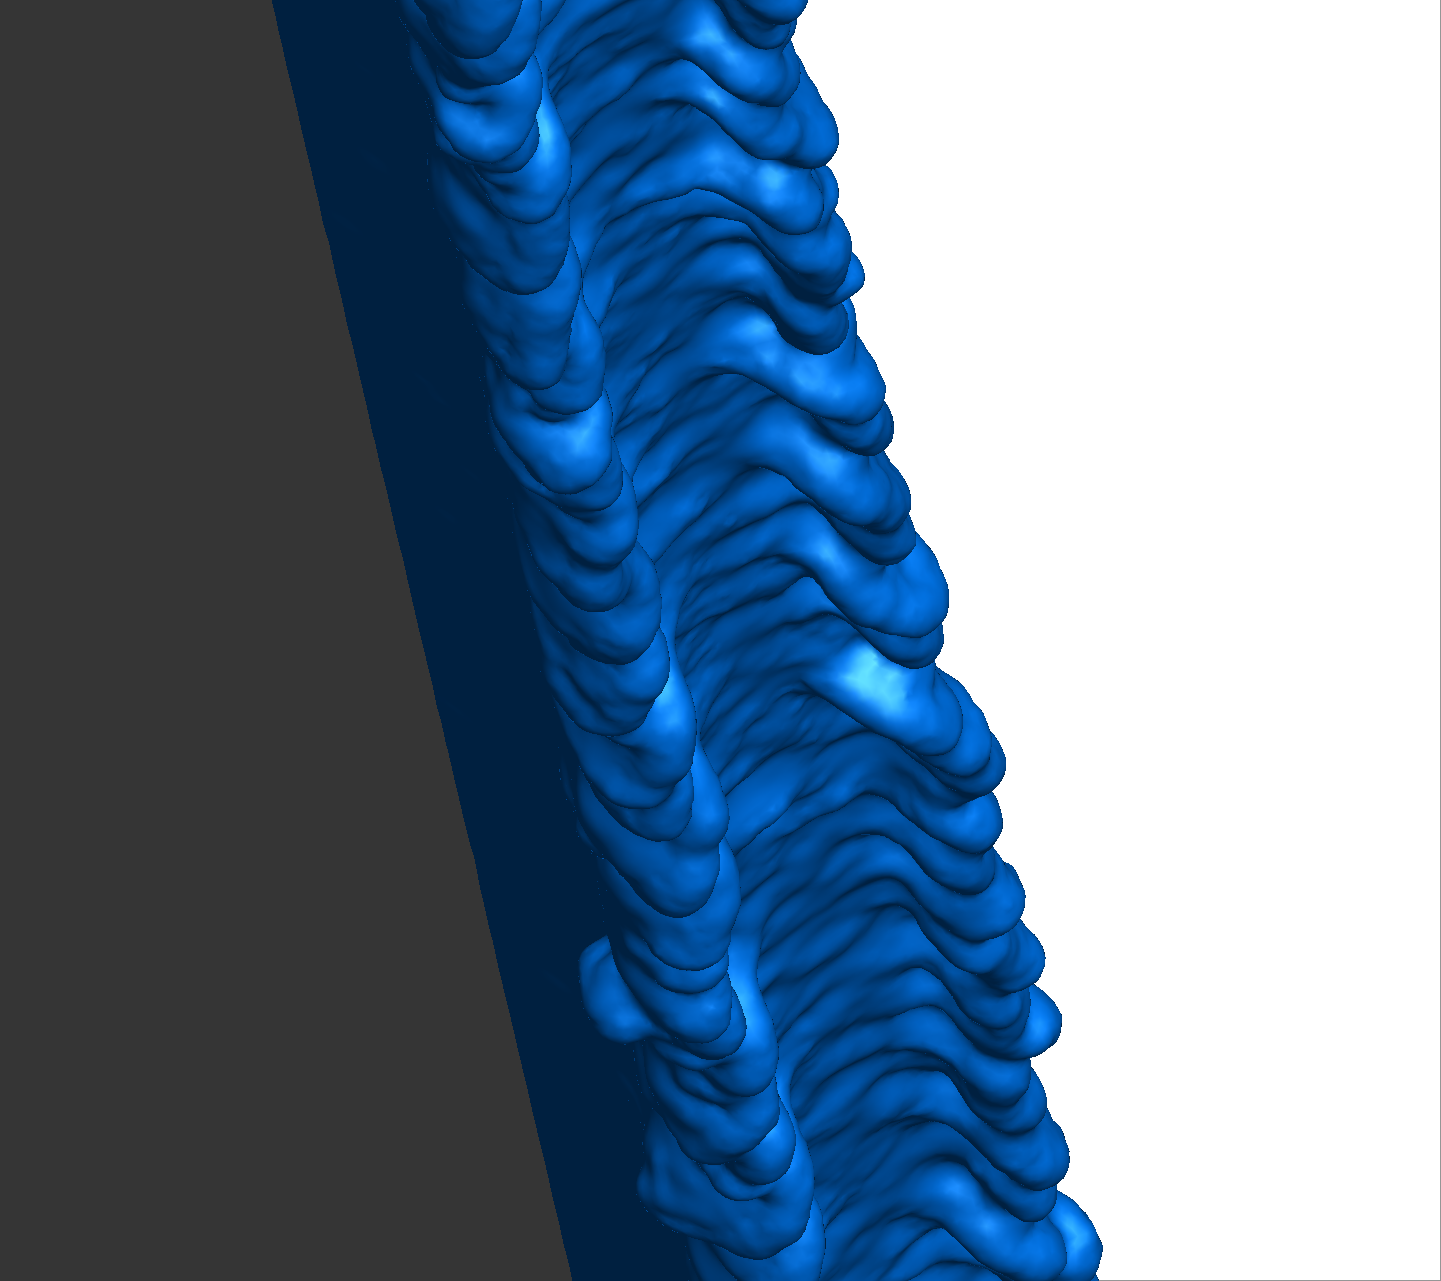
\includegraphics[
            width=\textwidth,
            height=2.25cm,
            keepaspectratio
        ]{FIGURES/CHAMPS_APPLICATIONS/DETERMINSTIC_ICING.png}

        \vspace{0.03cm}
        \textbf{\tiny Deterministic Icing}
    \end{column}
    \hfill

    % Stochastic icing
    \begin{column}{0.235\textwidth}
        \centering
        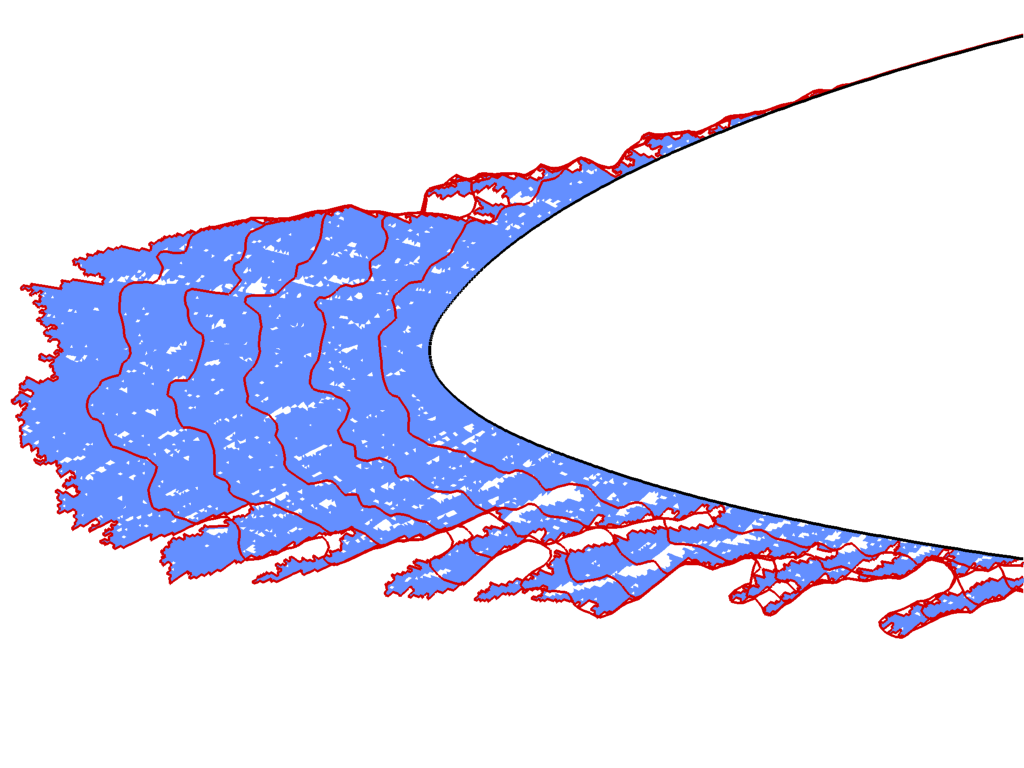
\includegraphics[
            width=\textwidth,
            height=2.25cm,
            keepaspectratio,
            trim={0cm 2cm 0cm 0cm},
            clip
        ]{FIGURES/CHAMPS_APPLICATIONS/STOCHASTIC_ICING.png}

        \vspace{0.03cm}
        \textbf{\tiny Stochastic Icing}
    \end{column}
    \hfill

    % DDES
    \begin{column}{0.235\textwidth}
        \centering
        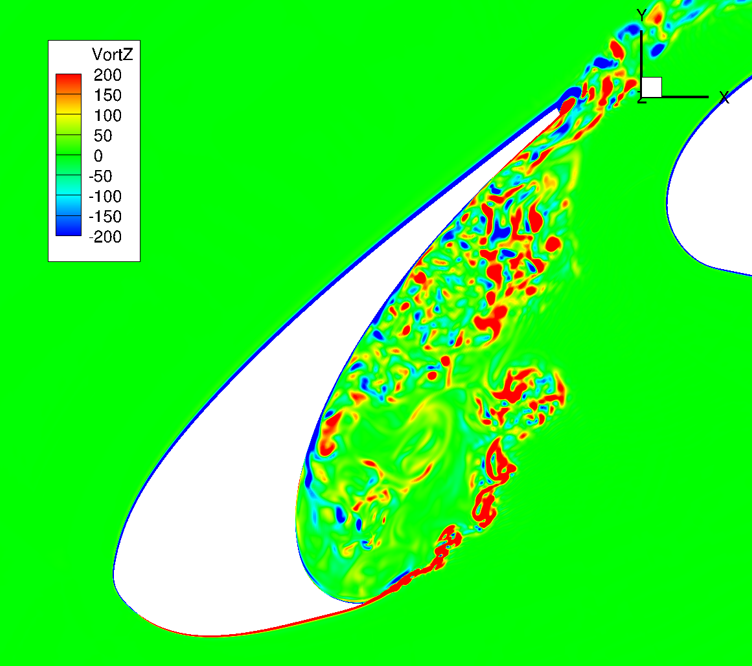
\includegraphics[
            width=\textwidth,
            height=2.25cm,
            keepaspectratio
        ]{FIGURES/CHAMPS_APPLICATIONS/DDES.png}

        \vspace{0.03cm}
        \textbf{\tiny Scale-Resolving CFD (DDES)}
    \end{column}
    \hfill

    % FSI
    \begin{column}{0.235\textwidth}
        \centering
        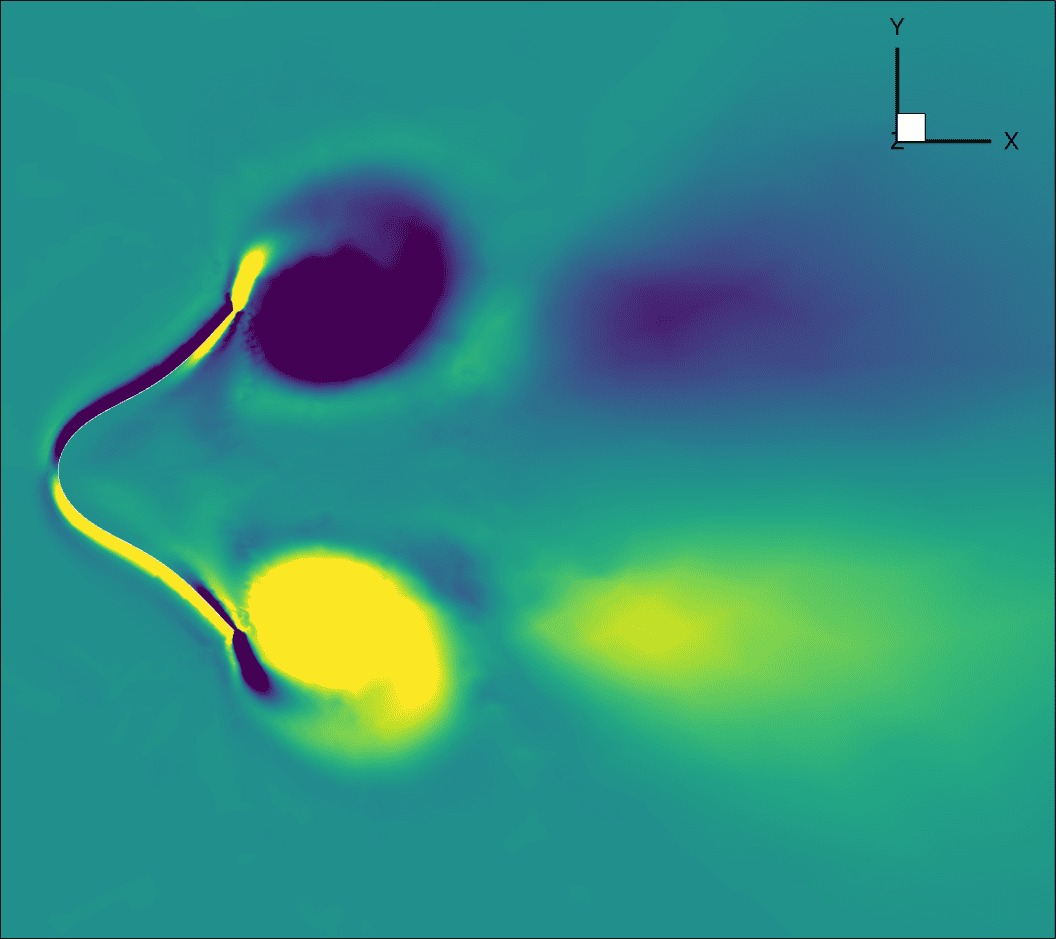
\includegraphics[
            width=\textwidth,
            height=2.25cm,
            keepaspectratio
        ]{FIGURES/CHAMPS_APPLICATIONS/FSI.jpeg}

        \vspace{0.03cm}
        \textbf{\tiny Fluid--Structure Interaction}
    \end{column}

\end{columns}

\vspace{0.15cm}

% ------------------------------------------------------------
% Contrails
% ------------------------------------------------------------

\begin{center}

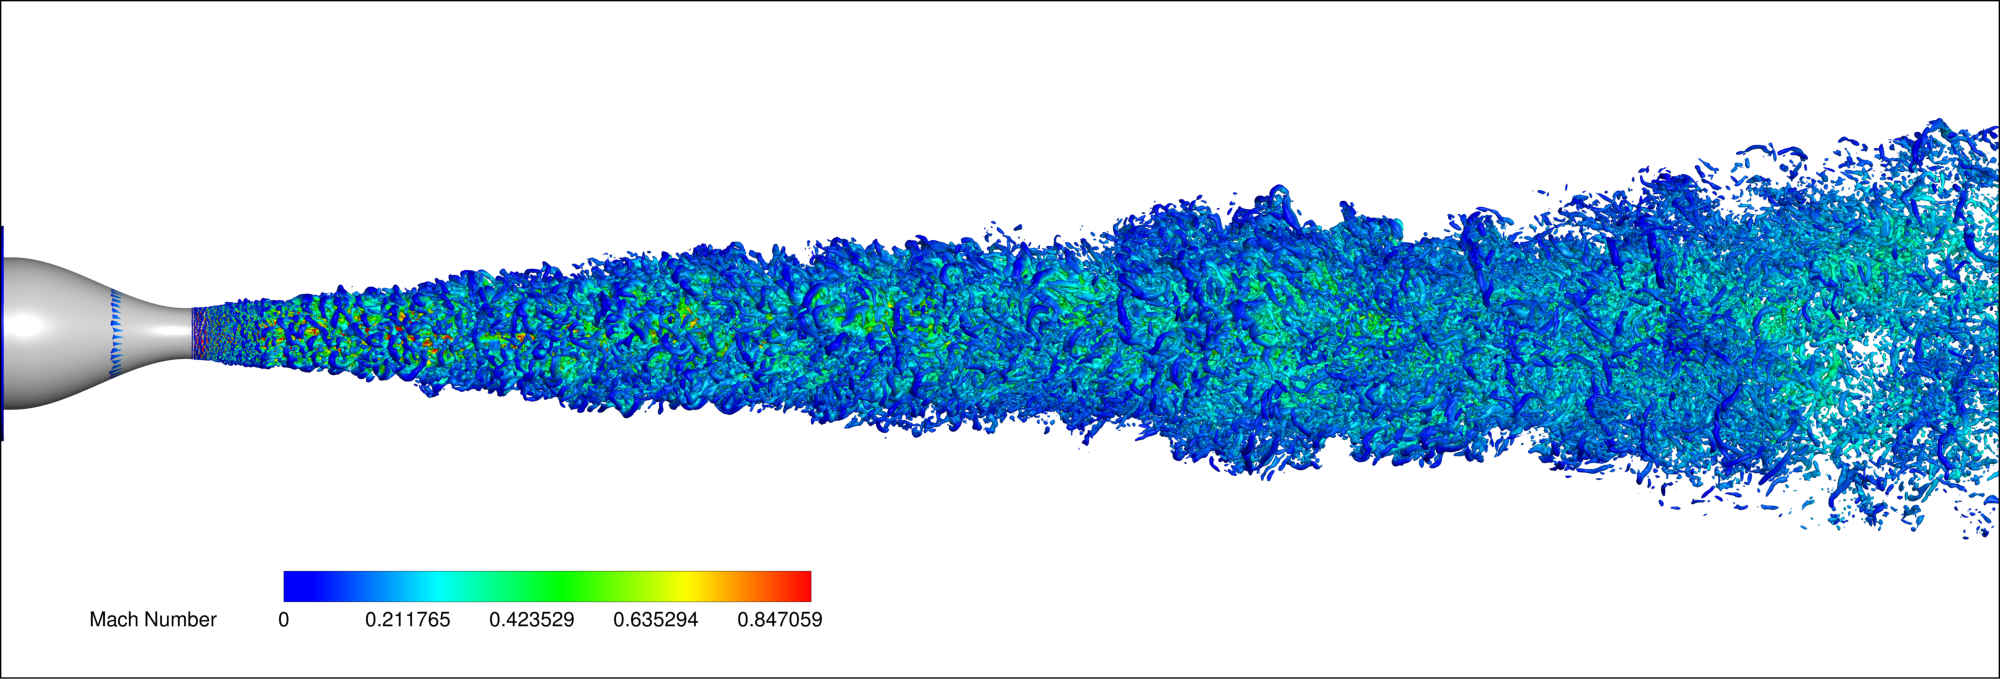
\includegraphics[
    height=1.90cm
]{FIGURES/CHAMPS_APPLICATIONS/MOTOR_EXIT.png}
\hspace{0.15cm}
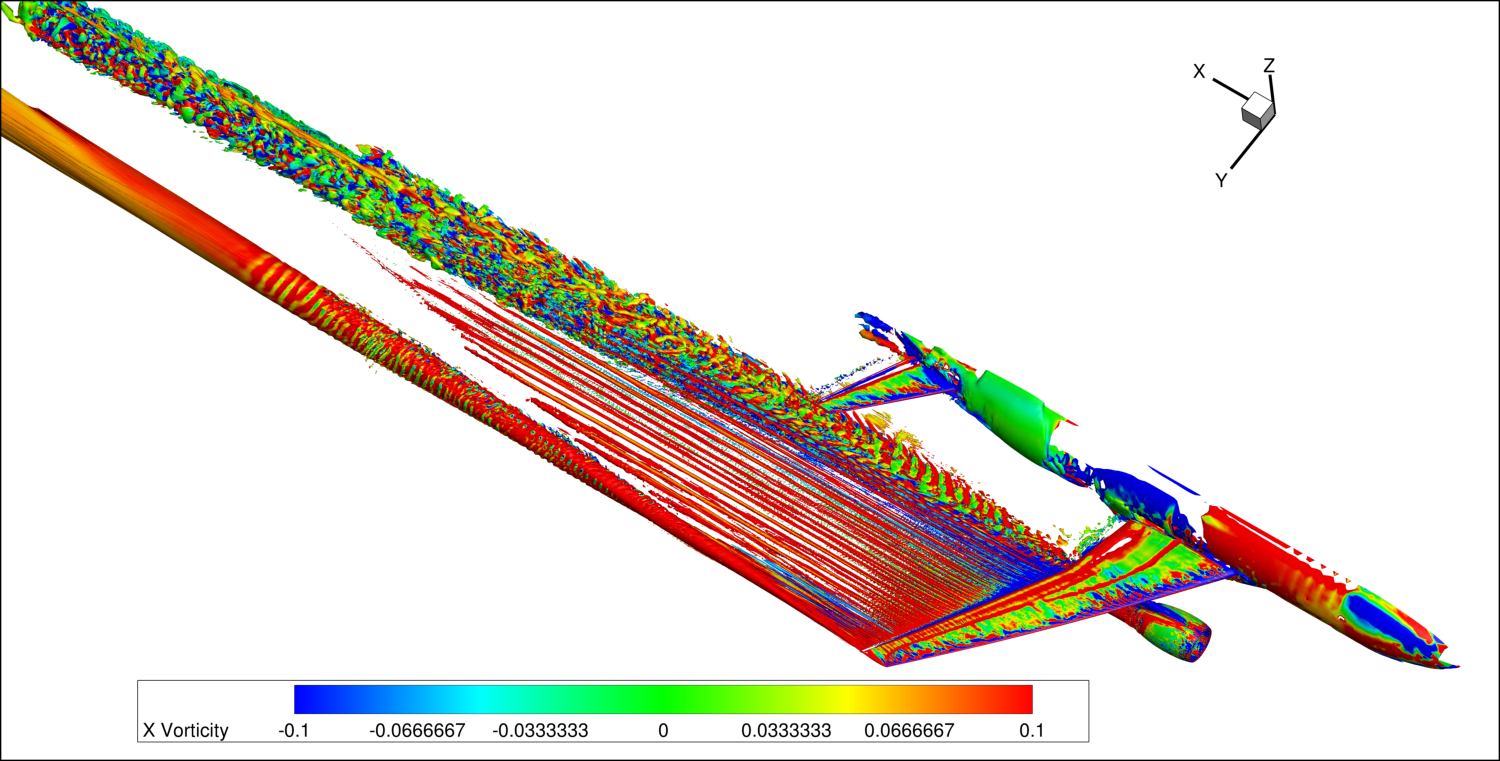
\includegraphics[
    height=1.90cm
]{FIGURES/CHAMPS_APPLICATIONS/VORTICITY_CRM.png}

\textbf{\tiny Contrails}$^{*}$
\end{center}

\vspace{-0.05cm}

% ------------------------------------------------------------
% CHAMPS Block
% ------------------------------------------------------------

\begin{block}{\scriptsize CHAMPS -- CHapel MultiPhysics Software}
\scriptsize

In-house unstructured finite-volume framework developed at
Polytechnique Montréal in Chapel for high-performance,
multi-fidelity and multiphysics aerospace simulations, providing a unified computational framework for all simulation capabilities.

\end{block}

\vspace{-0.05cm}

{\tiny
$^{*}$Contrail modeling developed in collaboration with Prof.\ Roberto Paoli.
}

\end{frame}
% ============================================================
% CHAMPS -- Icing Framework
% ============================================================

\begin{frame}[c]{\small CHAMPS -- Icing Framework}
\scriptsize

\centering

% ------------------------------------------------------------
% Icing Framework
% ------------------------------------------------------------

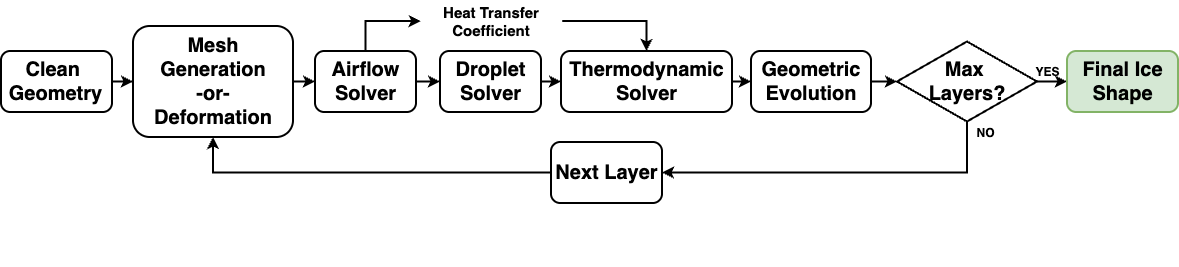
\includegraphics[
    width=0.88\textwidth,
    height=2.25cm,
    keepaspectratio
]{FIGURES/LS_FRAMEWORK/icingFramework.png}

\vspace{0.10cm}

% ------------------------------------------------------------
% Modeling Configuration
% ------------------------------------------------------------

\renewcommand{\arraystretch}{1.18}
\setlength{\tabcolsep}{5pt}

\begin{tabularx}{0.90\textwidth}{
    |>{\centering\arraybackslash}p{0.35\textwidth}
    |>{\centering\arraybackslash}X
    |>{\centering\arraybackslash}X|
}
\hline

\rowcolor{polymtlbluel}
\color{white}\textbf{Model / Method} &
\color{white}\textbf{NACA0012} &
\color{white}\textbf{ONERA M6} \\
\hline

Turbulence Model &
\multicolumn{2}{c|}{Spalart--Allmaras (SA)} \\
\hline

Heat-Transfer Method &
\multicolumn{2}{c|}{One Solution + $T_{\mathrm{rec}}$} \\
\hline

Droplet Model &
\multicolumn{2}{c|}{Eulerian / Lagrangian} \\
\hline

Droplet Drag Model &
\multicolumn{2}{c|}{Deformable Sphere} \\
\hline

SLD Corrections &
\multicolumn{2}{c|}{None} \\
\hline

Thermodynamic Model &
\multicolumn{2}{c|}{Messinger} \\
\hline

Ice Density &
$580~\mathrm{kg/m^3}$ &
$680~\mathrm{kg/m^3}$ \\
\hline

Surface Roughness &
$0.2667$ mm / $0.5334$ mm &
$1.0$ mm \\
\hline

Geometry Evolution &
\multicolumn{2}{c|}{Algebraic (Single-shot) / Level Set (Multilayer)} \\
\hline

Accretion Strategy &
\multicolumn{2}{c|}{Single-shot \& 5 Layers} \\
\hline

\end{tabularx}

\vspace{0.08cm}

% ------------------------------------------------------------
% Numerical Details
% ------------------------------------------------------------

\begin{flushleft}
\tiny
\textbf{*} Flow equations use Roe convective fluxes with the
Venkatakrishnan limiter; Eulerian droplet equations use an upwind
scheme with the Van Albada limiter. Lagrangian simulations were
performed to verify the Eulerian collection-efficiency predictions.
\end{flushleft}

\end{frame}

% ============================================================
% CHAMPS -- MULTILAYER ICE-ACCRETION APPROACH
% ============================================================

\begin{frame}[c]{\small CHAMPS -- Multilayer Ice-Accretion Approach}
\scriptsize

\vspace{-0.10cm}

\centering

% ============================================================
% LEFT -- LEVEL-SET FORMULATION
% ============================================================
\begin{minipage}[t]{0.40\textwidth}
\vspace{0pt}

\begin{block}{\scriptsize Level-Set Formulation}

The ice--air interface is implicitly represented by the
\textbf{zero level set} of a signed-distance function $\phi$
\cite{OSHER2004,FROLKOVIC2015214,lavoieLevelSet}:

\vspace{-0.10cm}

\[
\frac{\partial \phi}{\partial t}
+ \nabla \cdot (\phi \boldsymbol{V})
- \phi \nabla \cdot \boldsymbol{V}
= 0,
\qquad
\boldsymbol{V}
=
\frac{h_{\mathrm{ice}}}{\Delta t_{\mathrm{layer}}}
\,\boldsymbol{n}_{\phi_0}.
\]

\vspace{-0.10cm}

\begin{itemize}
    \setlength{\itemsep}{0.45cm}

    \item $\boldsymbol{n}_{\phi_0}$ denotes the local level-set normal
    computed from the initial wall-distance field $\phi_0$.

    \item The predicted ice thickness defines the interface advection velocity
    $\boldsymbol{V}$.

    \item The interface is advected through unsteady time stepping
    until either the prescribed icing time or the predicted ice volume is reached.

    \item The updated ice geometry is extracted from the
    $\boldsymbol{\phi=0}$ isosurface using the open-source
    Mmg library \cite{dapogny2014mmg}, and used for the next accretion layer.

\end{itemize}

\end{block}

\end{minipage}%
\hspace{0.03\textwidth}%
% ============================================================
% RIGHT -- ILLUSTRATIONS
% ============================================================
\begin{minipage}[t]{0.50\textwidth}
\vspace{0pt}
\centering

% ------------------------------------------------------------
% Level-set / interface illustration
% ------------------------------------------------------------
\textbf{\scriptsize Ice--Air Interface}

\vspace{0.03cm}

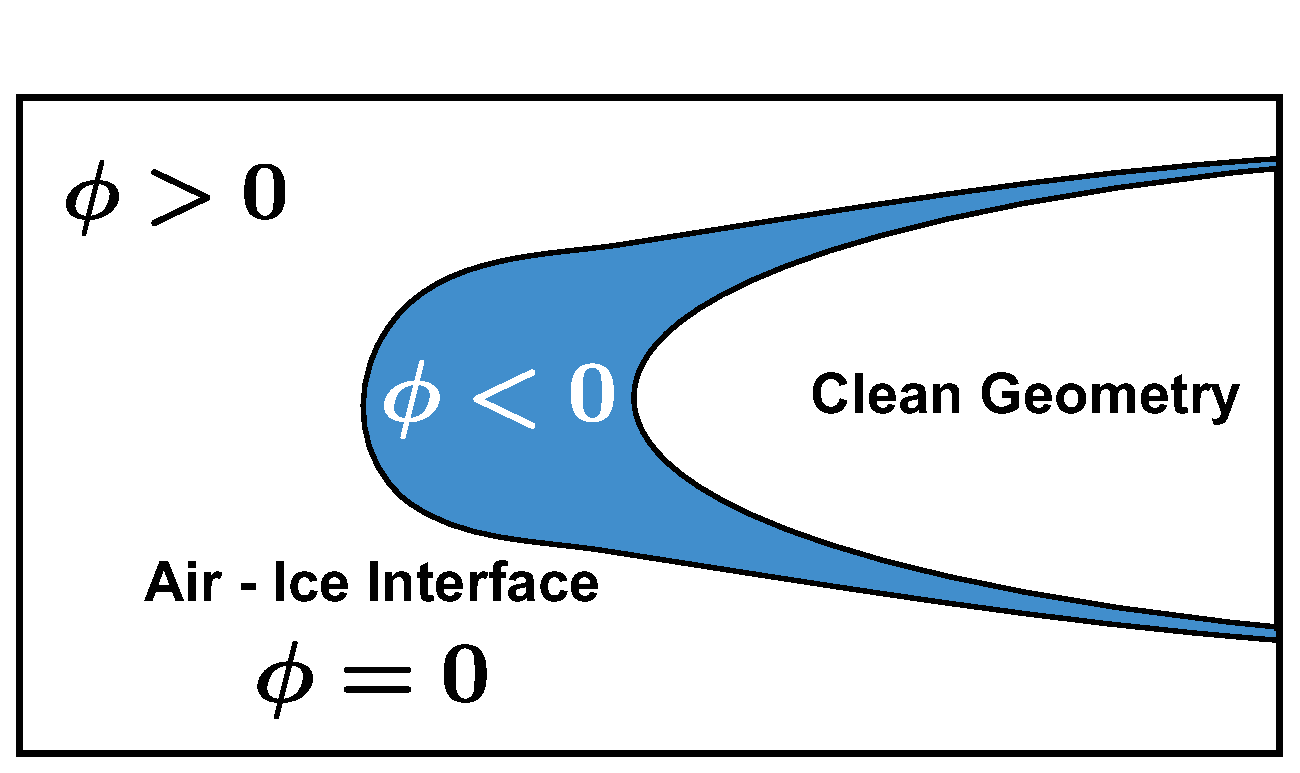
\includegraphics[
    width=\textwidth,
    height=2.65cm,
    keepaspectratio
]
{FIGURES/LS_FRAMEWORK/ICE_AIR_INTERFACE.eps}

\vspace{0.12cm}

% ------------------------------------------------------------
% Complex 3D ice geometry
% ------------------------------------------------------------
\textbf{\scriptsize Extracted 3D Ice Geometry}

\vspace{0.03cm}

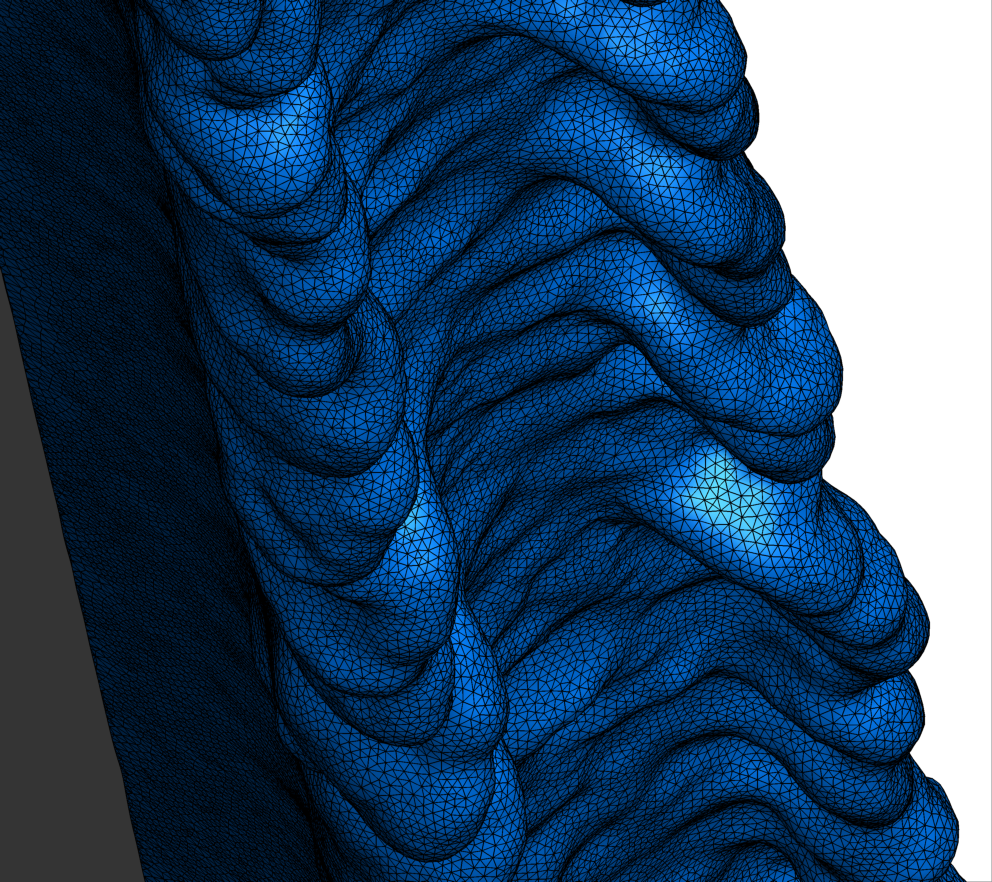
\includegraphics[
    width=\textwidth,
    height=4.05cm,
    keepaspectratio
]
{FIGURES/LS_FRAMEWORK/CLIPPED_ICE_SHAPE_CASE_362_3.png}

\end{minipage}

\end{frame}
\section[NACA0012]{\textbf{NACA0012 Icing Results}}

% ============================================================
% NACA0012 -- ICING RESULTS
% ============================================================

\begin{frame}[plain]
    \centering
    \vfill

    {\LARGE\bfseries NACA0012 RESULTS}

    \vfill
\end{frame}

% ============================================================
% NACA0012 -- Integrated Aerodynamic Coefficients
% ============================================================

\begin{frame}{\small NACA0012 -- Integrated Aerodynamic Coefficients}
\scriptsize

\vspace{-0.1cm}

\begin{columns}[T,onlytextwidth]

% ------------------------------------------------------------
% CL
% ------------------------------------------------------------
\begin{column}{0.33\textwidth}
    \centering
    \textbf{$C_L$}

    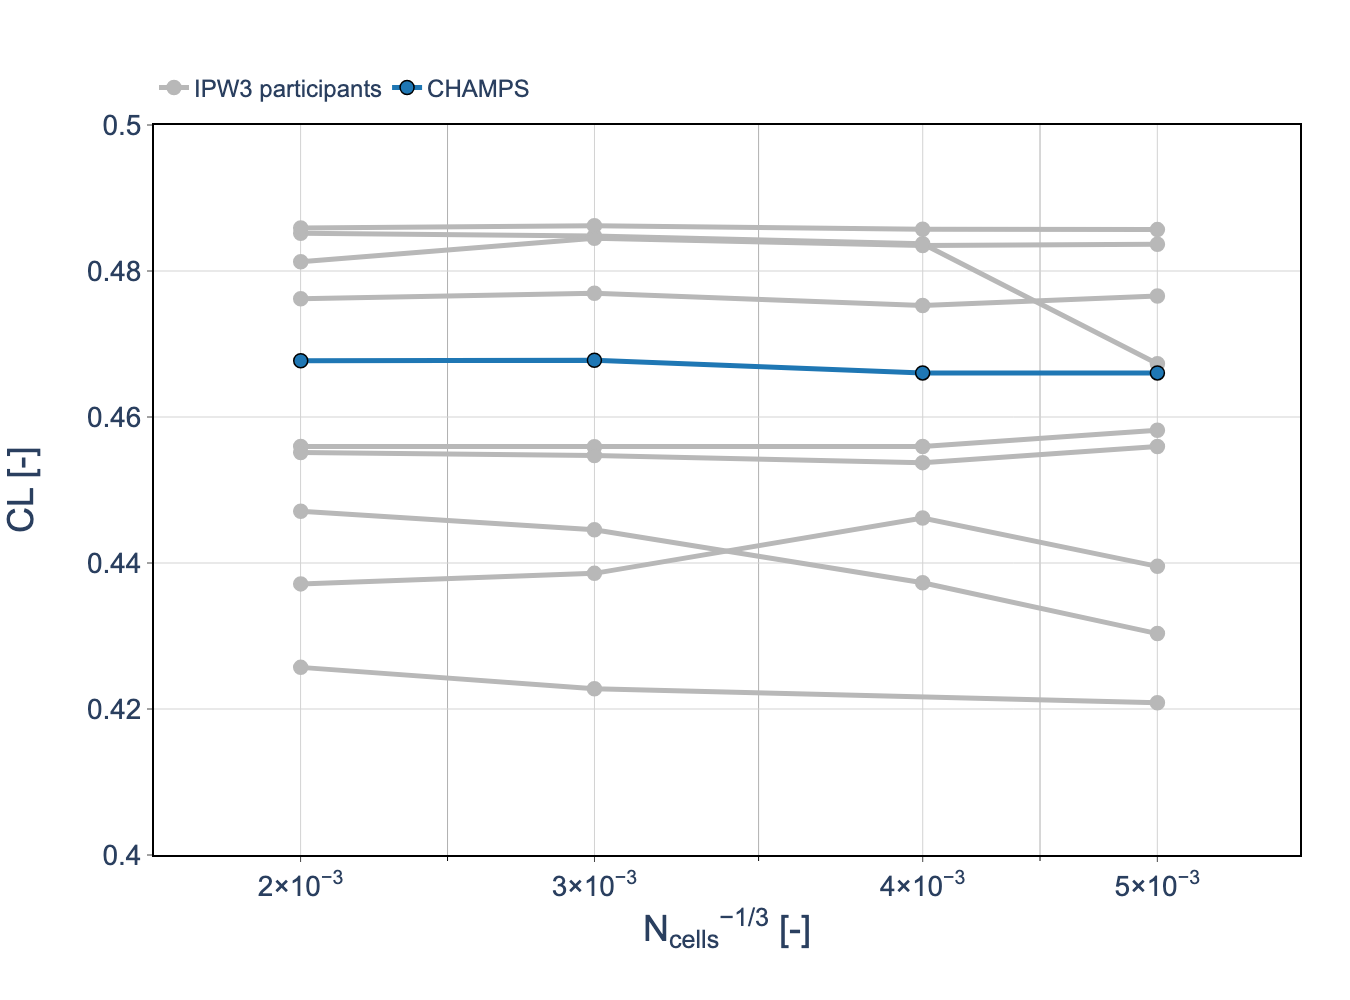
\includegraphics[
        width=\textwidth,
        trim={0cm 0cm 1cm 2.6cm},
        clip
    ]
    {FIGURES/NACA0012/AERODYNAMIC/tc_naca0012_ae3932_cl_vs_n_all_roughness.png}
\end{column}

% ------------------------------------------------------------
% CD
% ------------------------------------------------------------
\begin{column}{0.33\textwidth}
    \centering
    \textbf{$C_D$}

    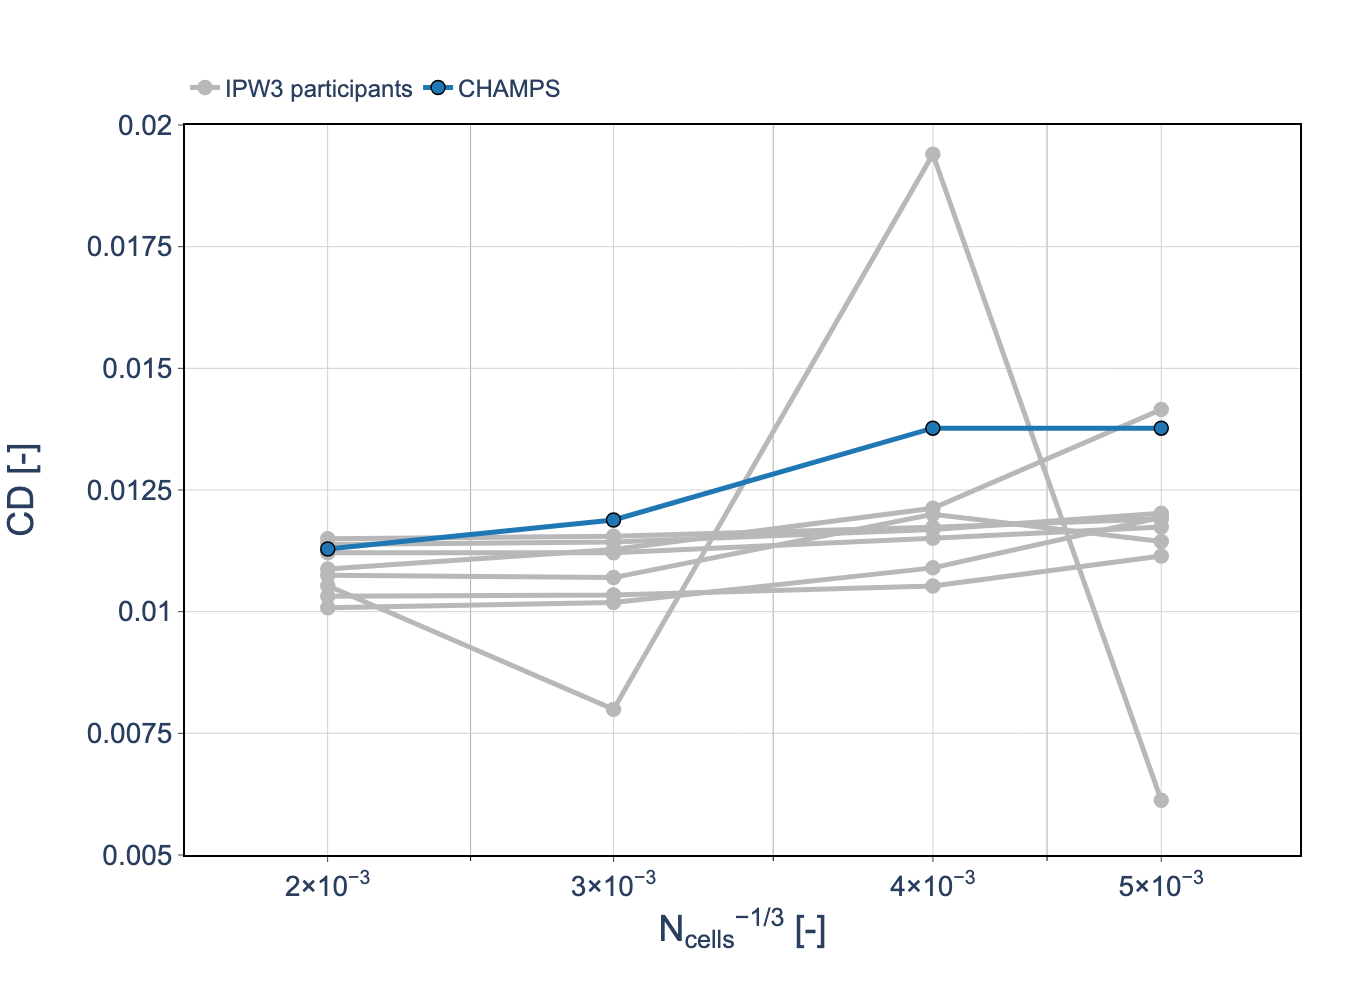
\includegraphics[
        width=\textwidth,
        trim={0cm 0cm 1cm 2.6cm},
        clip
    ]
    {FIGURES/NACA0012/AERODYNAMIC/tc_naca0012_ae3932_cd_vs_n_all_roughness.png}
\end{column}

% ------------------------------------------------------------
% CM
% ------------------------------------------------------------
\begin{column}{0.33\textwidth}
    \centering
    \textbf{$C_M$}

    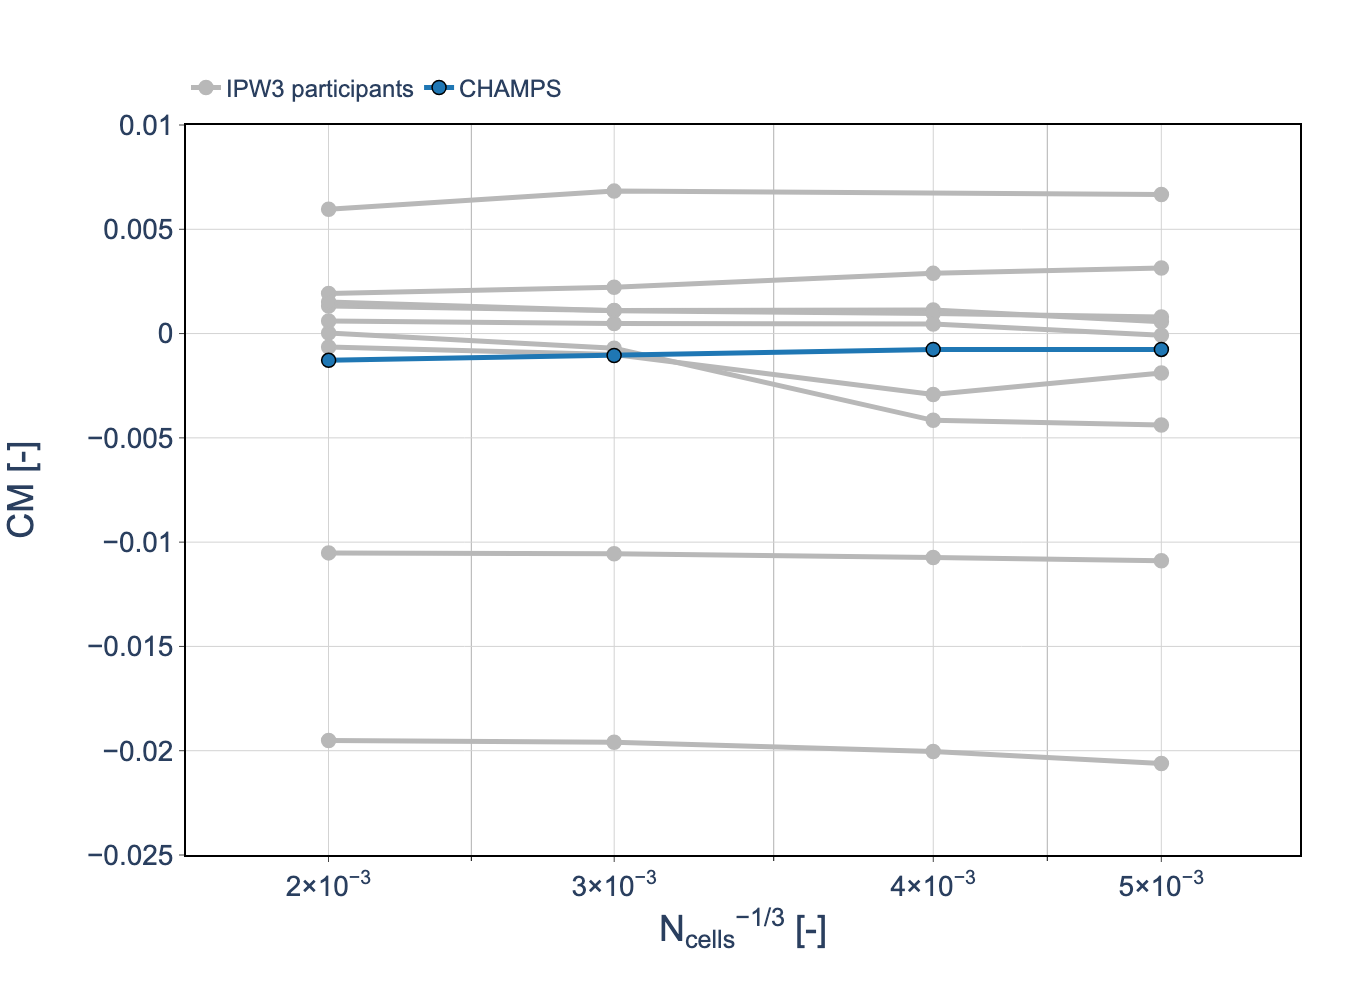
\includegraphics[
        width=\textwidth,
        trim={0cm 0cm 1cm 2.6cm},
        clip
    ]
    {FIGURES/NACA0012/AERODYNAMIC/tc_naca0012_ae3932_cmy_vs_n_all_roughness.png}
\end{column}

\end{columns}

\vspace{-0.10cm}

\begin{center}
\renewcommand{\arraystretch}{1.20}
\setlength{\tabcolsep}{6pt}

\begin{tabular}{lccc}
\toprule
& $\mathbf{C_L}$ & $\mathbf{C_D}$ & $\mathbf{C_M}$ \\
\midrule

\textbf{CHAMPS}
& 0.4677
& 0.01129
& -0.00128 \\

\textbf{IPW3 L1 Median}
& 0.4657
& 0.01088
& -0.00295 \\

\textbf{Difference}
& +0.43\%
& +3.77\%
& +0.00167 \\

\bottomrule
\end{tabular}
\end{center}

\vspace{-0.15cm}

\begin{block}{\scriptsize Integrated Aerodynamic Coefficients Assessment}
CHAMPS predicts integrated aerodynamic coefficients close to the IPW3 L1
median. $C_D$ exhibits the greatest sensitivity to spatial grid refinement.
\end{block}

\end{frame}


% ============================================================
% NACA0012 -- Pressure Distribution
% ============================================================

\begin{frame}{\small NACA0012 -- Pressure-Coefficient Distribution}
\scriptsize

\vspace{-0.15cm}

\begin{columns}[T,onlytextwidth]

% ------------------------------------------------------------
% Cp vs x
% ------------------------------------------------------------
\begin{column}{0.50\textwidth}
    \centering
    \textbf{$C_p$ vs. $x$}

    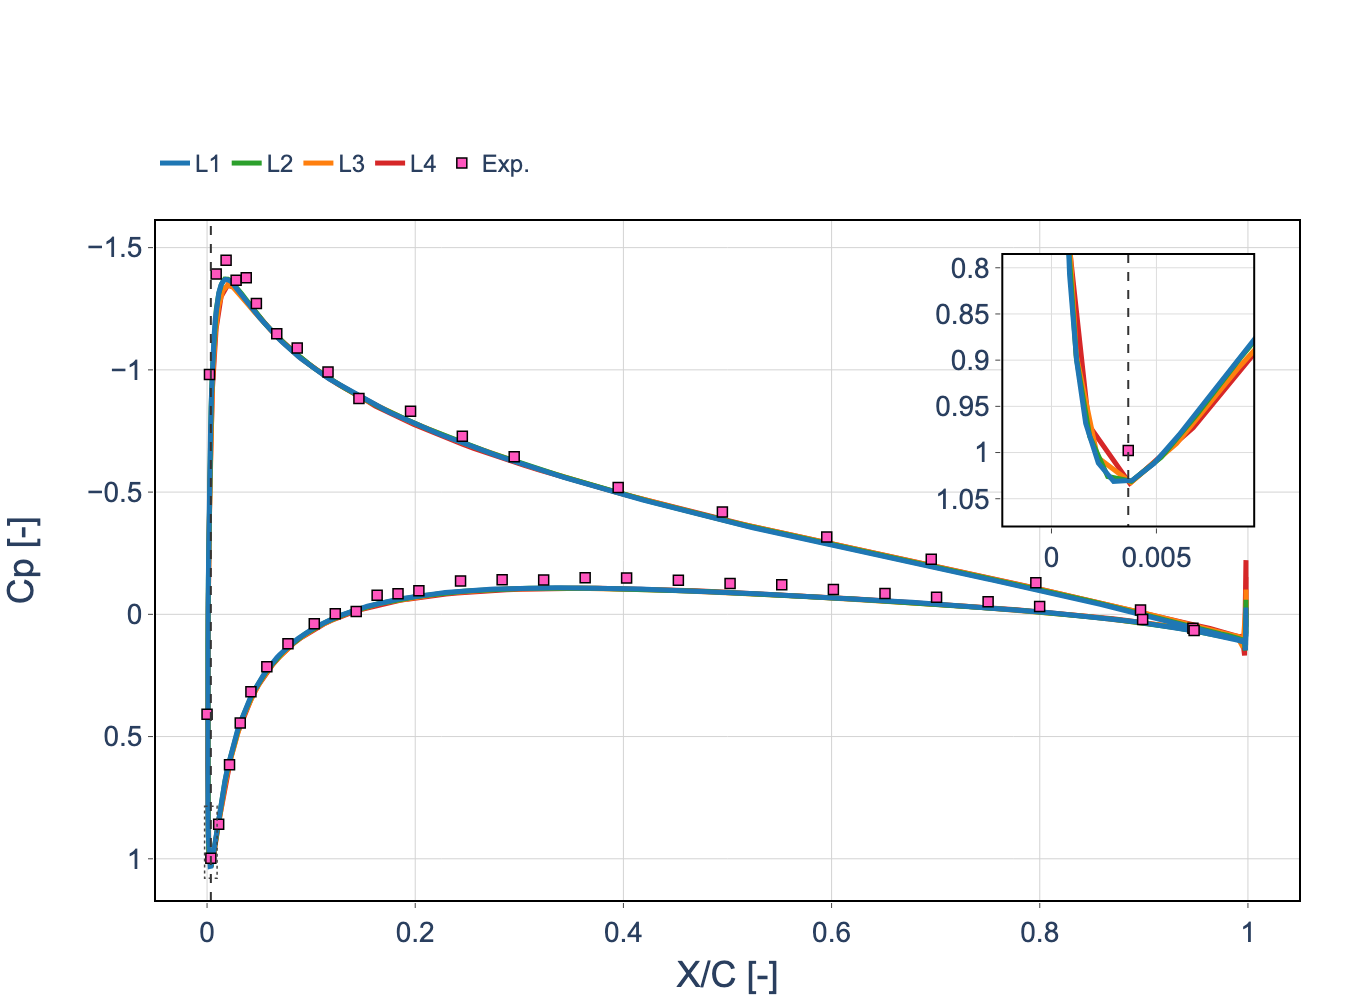
\includegraphics[
        width=\textwidth,
        trim={0cm 0cm 1cm 3.0cm},
        clip
    ]
    {FIGURES/NACA0012/AERODYNAMIC/tc_naca0012_ae3932_L1_cp_vs_x_slice_0p9144_all_roughness.png}
\end{column}

% ------------------------------------------------------------
% Cp vs s
% ------------------------------------------------------------
\begin{column}{0.50\textwidth}
    \centering
    \textbf{$C_p$ vs. $s$}

    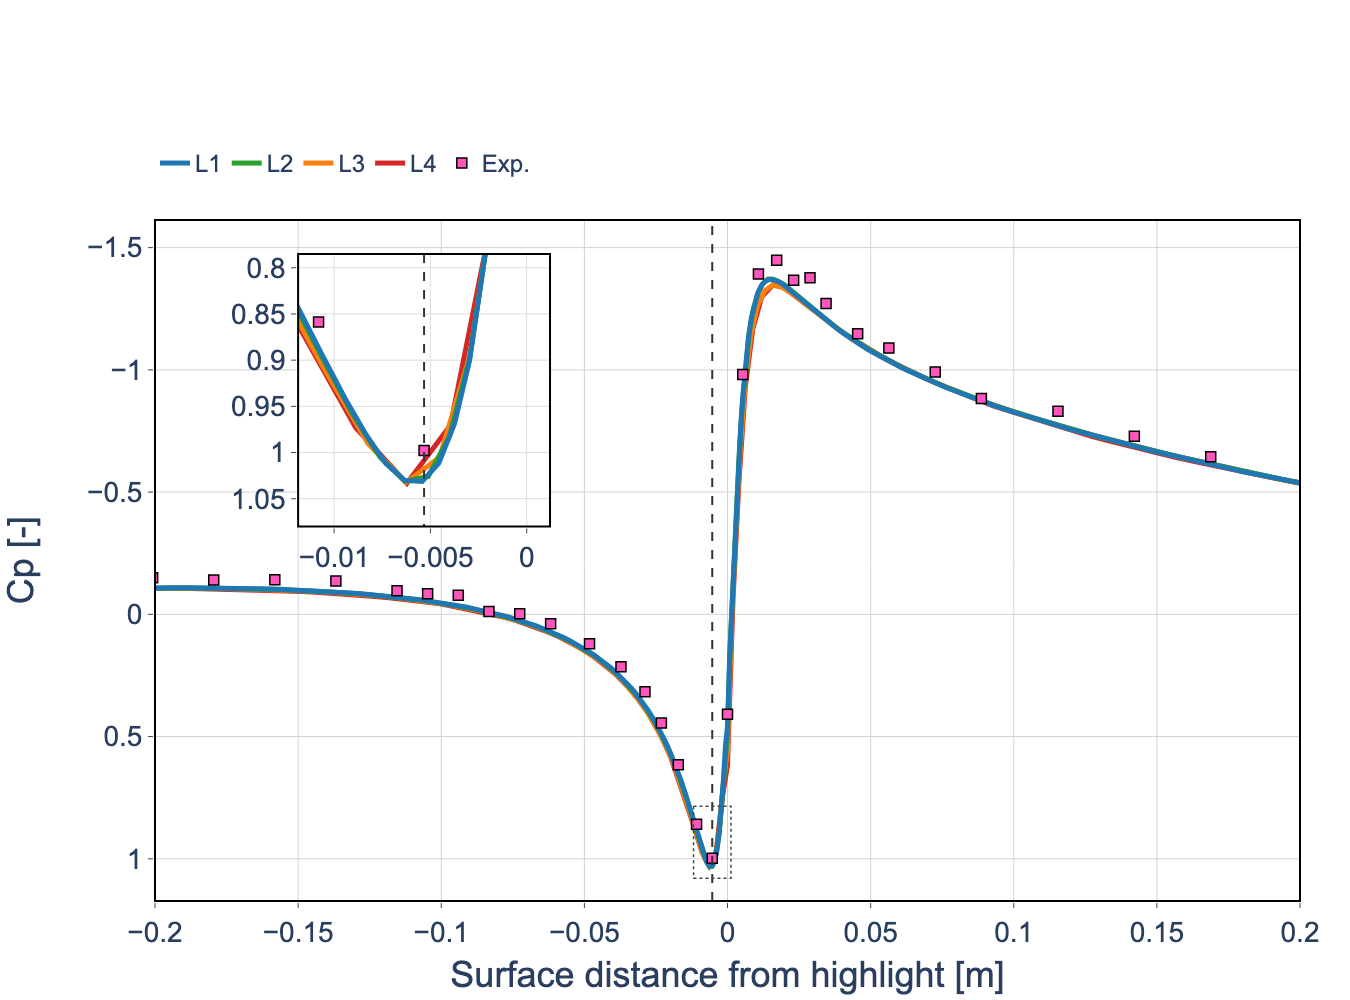
\includegraphics[
        width=\textwidth,
        trim={0cm 0cm 1cm 3.0cm},
        clip
    ]
    {FIGURES/NACA0012/AERODYNAMIC/tc_naca0012_ae3932_L1_cp_vs_s_slice_0p9144_all_roughness.png}
\end{column}

\end{columns}

\vspace{-0.05cm}

\begin{block}{\scriptsize Pressure-Coefficient Assessment}
CHAMPS predictions are in good agreement with the experimental pressure distribution across all grid levels.
\end{block}

\end{frame}


% ============================================================
% NACA0012 -- Droplet Impingement
% ============================================================

\begin{frame}{\small NACA0012 -- Droplet Impingement}
\scriptsize

\vspace{-0.15cm}

\begin{columns}[T,onlytextwidth]

% ------------------------------------------------------------
% Droplet-Bin Refinement
% ------------------------------------------------------------
\begin{column}{0.50\textwidth}
    \centering

    \textbf{Droplet-Bin Refinement -- L1, Eulerian}

    \vspace{-0.05cm}

    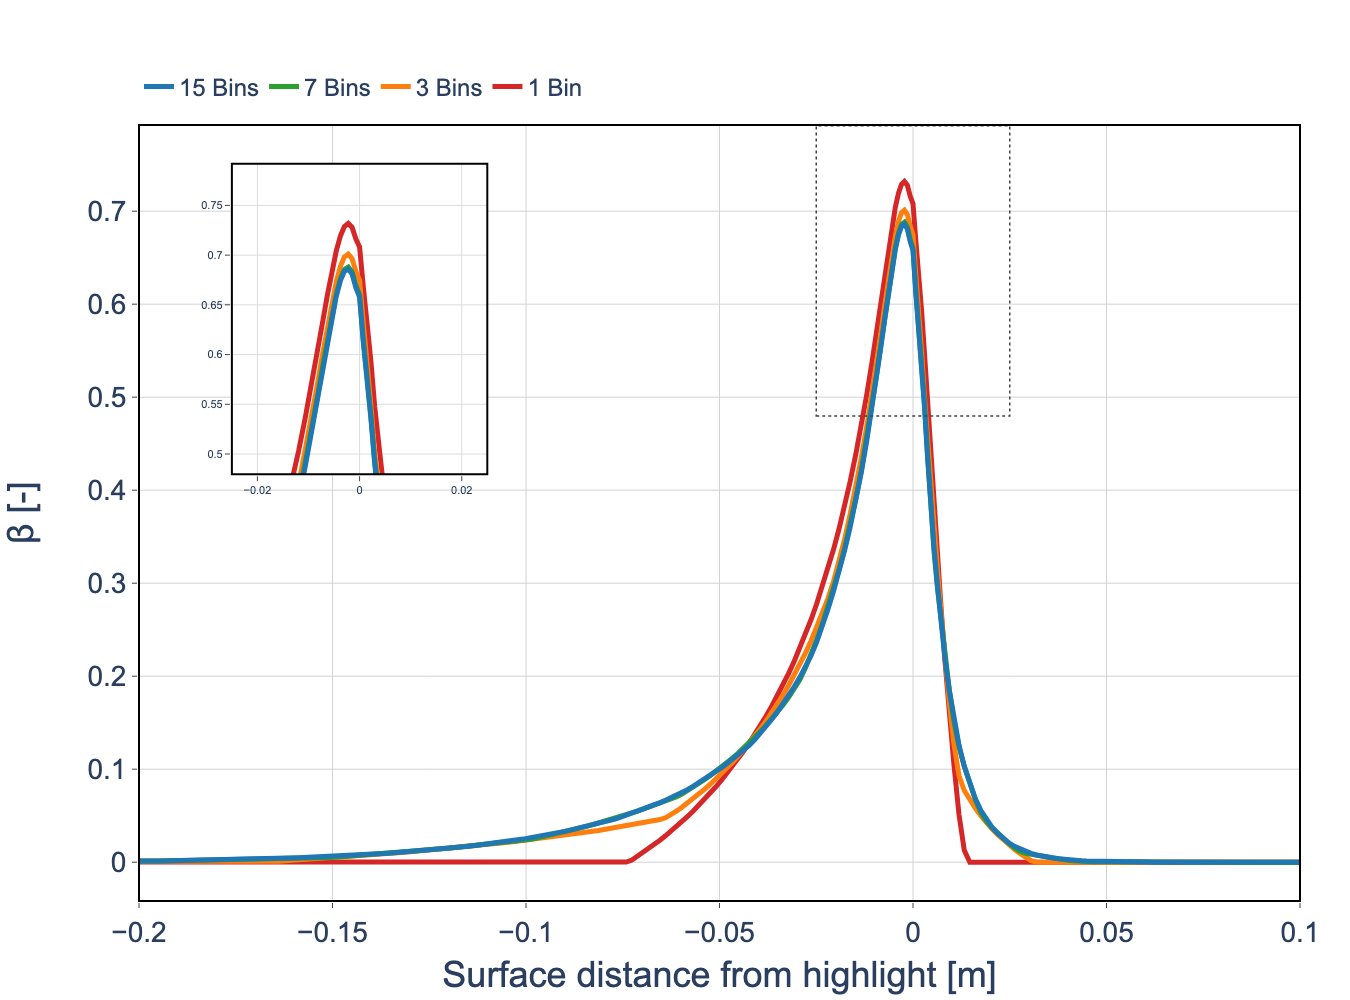
\includegraphics[
        trim={0cm 0cm 1cm 2.6cm},
        clip,
        width=\textwidth
    ]
    {FIGURES/NACA0012/IMPINGEMENT/tc_naca0012_ae3932_beta_bins07_vs_s_slice_0p9144_all_roughness_eulerian_grid_levels.png}

\end{column}

% ------------------------------------------------------------
% Eulerian vs Lagrangian
% ------------------------------------------------------------
\begin{column}{0.50\textwidth}
    \centering

    \textbf{Eulerian vs. Lagrangian -- L1, 7 Bins}

    \vspace{-0.05cm}

    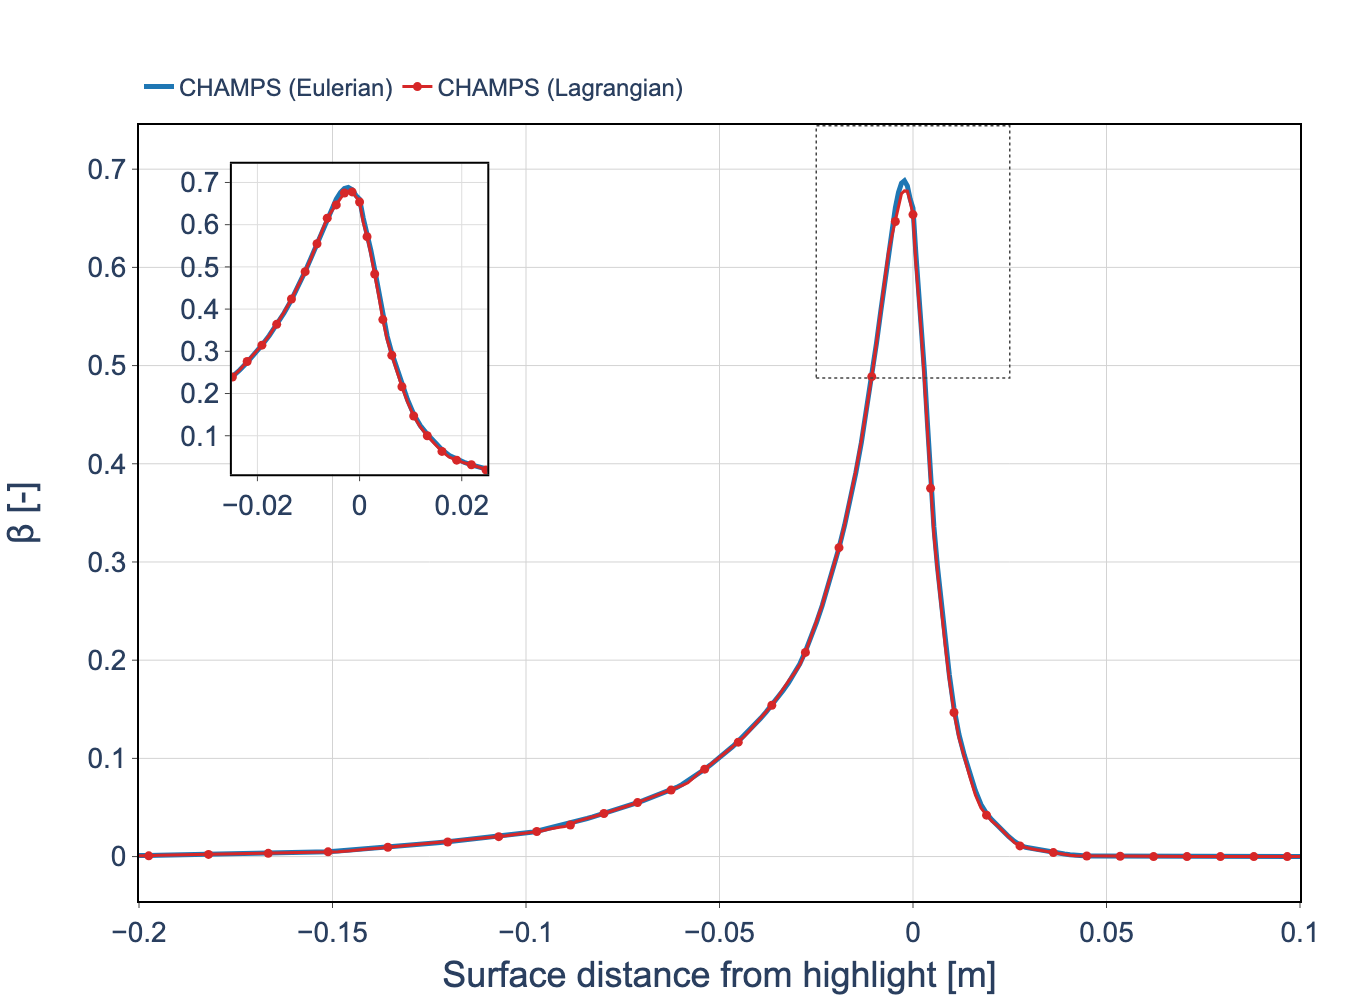
\includegraphics[
        trim={0cm 0cm 1cm 2.6cm},
        clip,
        width=\textwidth
    ]
    {FIGURES/NACA0012/IMPINGEMENT/tc_naca0012_ae3932_L1_beta_bins07_vs_s_slice_0p9144_all_roughness.png}

\end{column}

\end{columns}

\vspace{-0.15cm}

\begin{block}{\scriptsize Impingement Assessment}
\begin{itemize}
    \item Droplet-bin refinement highly affects the peak collection efficiency and impingement limits.
    \item Close agreement between the CHAMPS Eulerian and Lagrangian formulations, with minor differences near peak collection efficiency.
\end{itemize}
\end{block}

\end{frame}


% ============================================================
% NACA0012 -- Ice Mass
% ============================================================

\begin{frame}{\small NACA0012 -- Ice-Mass Prediction (15 Bins)}
\scriptsize

\vspace{-0.2cm}
\centering
% ------------------------------------------------------------
% AE3932 -- Ice Mass
% ------------------------------------------------------------
\begin{minipage}[t]{0.43\textwidth}
    \vspace{0pt}
    \centering

    \textbf{AE3932}

    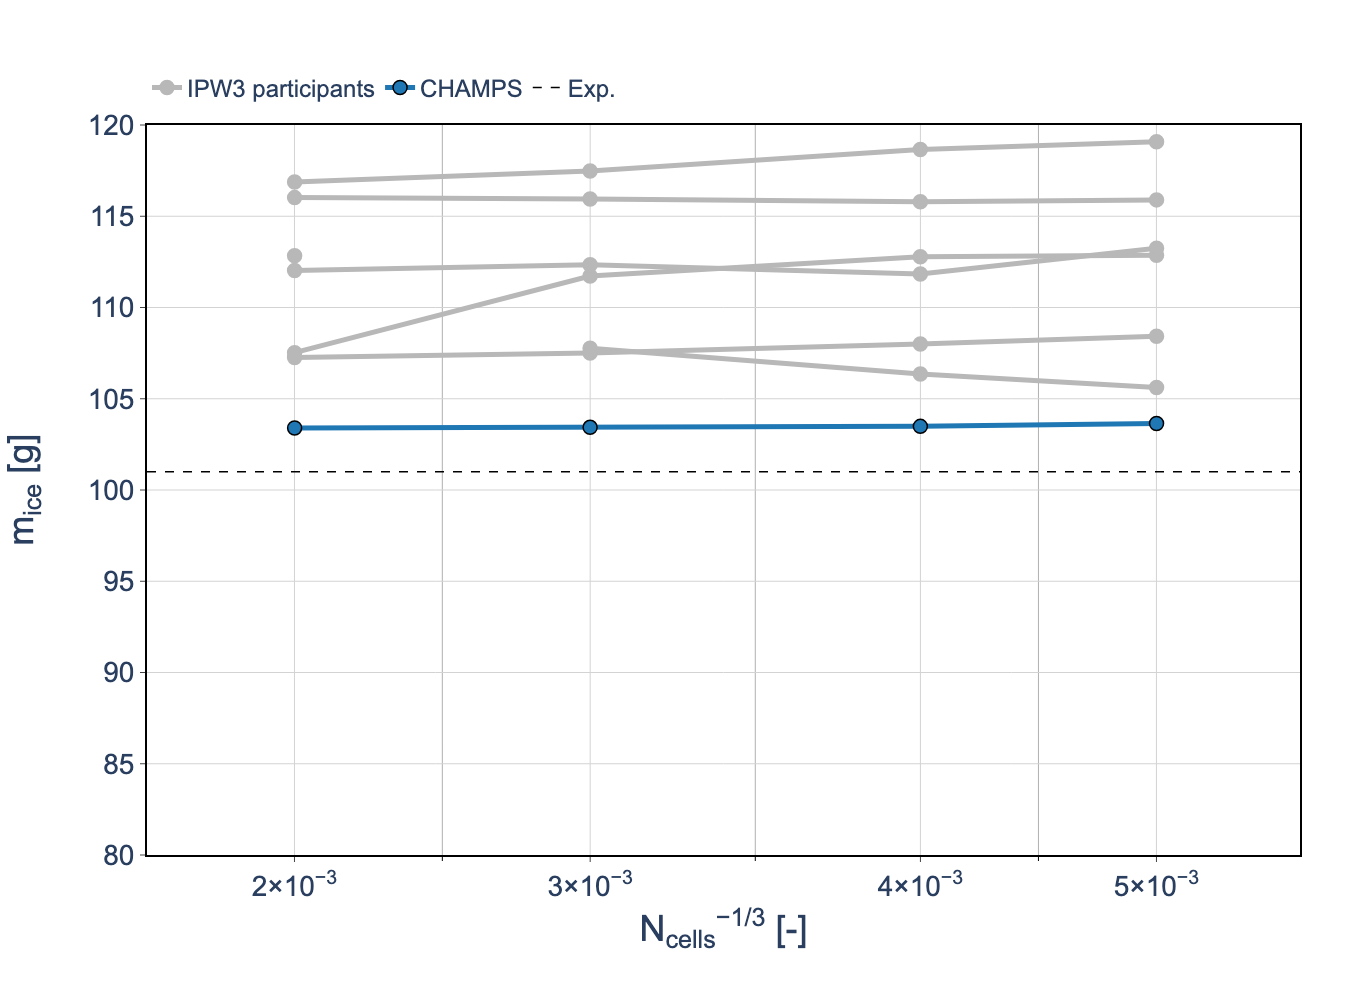
\includegraphics[
        width=\textwidth,
        trim={0cm 0cm 1cm 0.8cm},
        clip
    ]
    {FIGURES/NACA0012/ICE_ACCRETION/tc_naca0012_ae3932_ice_mass_vs_n_unspecified_bins15_all_grid_levels.png}
\end{minipage}%
\hspace{0.02\textwidth}%
% ------------------------------------------------------------
% AE3933 -- Ice Mass
% ------------------------------------------------------------
\begin{minipage}[t]{0.43\textwidth}
    \vspace{0pt}
    \centering

    \textbf{AE3933}

    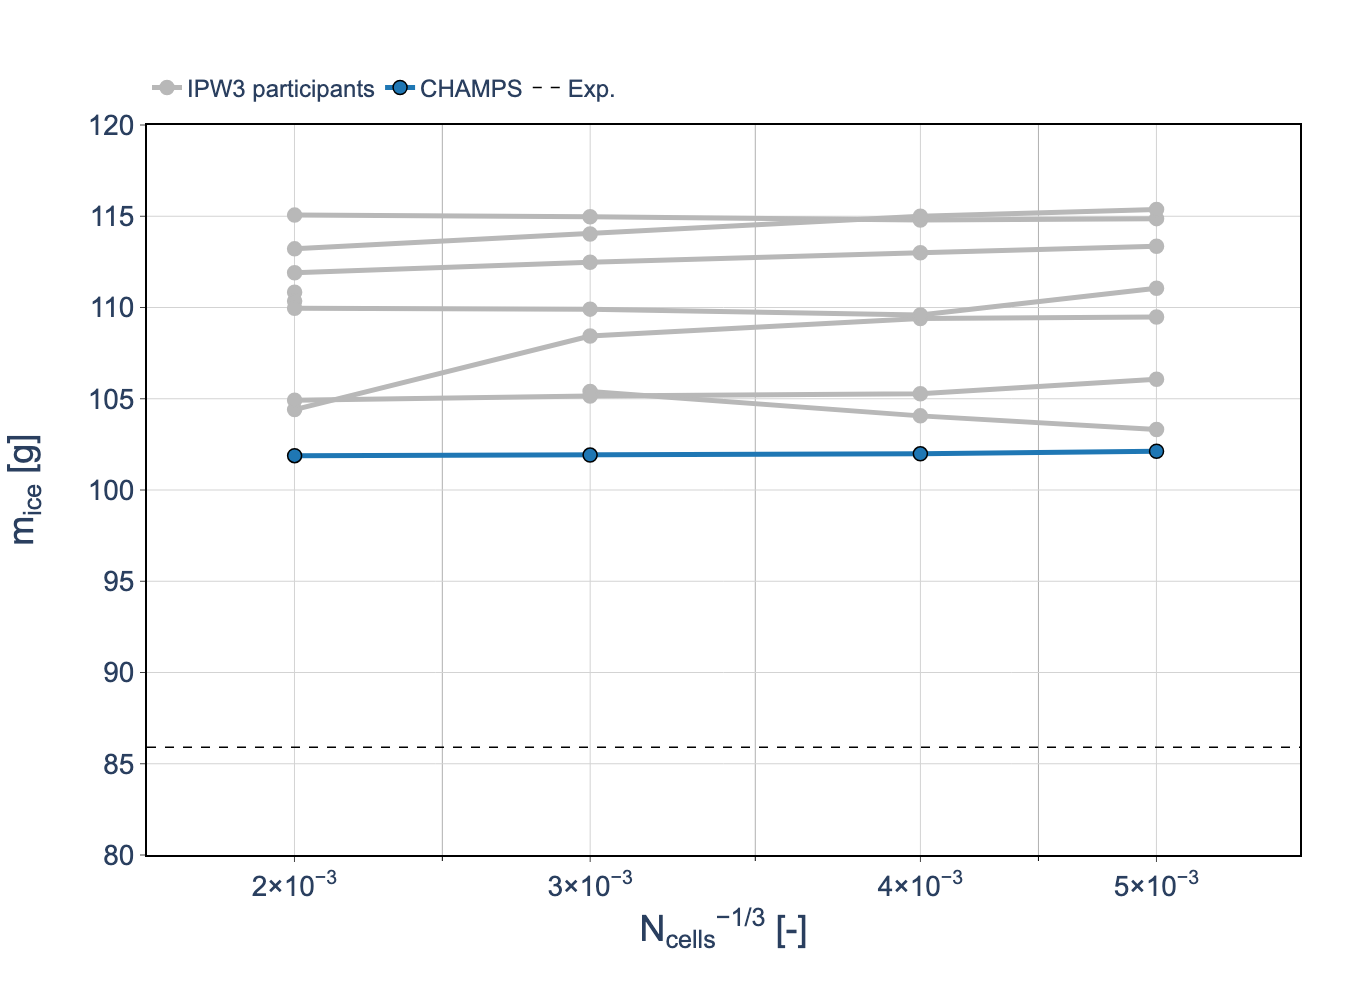
\includegraphics[
        width=\textwidth,
        trim={0cm 0cm 1cm 0.8cm},
        clip
    ]
    {FIGURES/NACA0012/ICE_ACCRETION/tc_naca0012_ae3933_ice_mass_vs_n_unspecified_bins15_all_grid_levels.png}
\end{minipage}

\vspace{-0.2cm}

% ------------------------------------------------------------
% Assessment
% ------------------------------------------------------------
\begin{block}{\scriptsize Ice-Accretion Assessment}
\begin{itemize}
    \item With the 15-bin distribution, CHAMPS predicts the AE3932 ice mass in very good agreement with the experimental value and exhibits limited sensitivity to spatial grid refinement.
    
    \item CHAMPS predicts a slightly lower ice mass for AE3933, with a reduction of approximately $1.5$ g ($\sim1.5\%$) relative to AE3932, compared with the approximately $15\%$ reduction measured experimentally.
    
    \item Approximately $88$--$90\%$ of the impinging water mass freezes into ice, with the remaining water mass lost through evaporation.
\end{itemize}
\end{block}

\end{frame}


% ============================================================
% NACA0012 -- Single-Layer Ice Shapes
% ============================================================

\begin{frame}{\small NACA0012 -- Single-Layer Ice-Shape Comparison}
\scriptsize

\vspace{-0.15cm}

\begin{columns}[T,onlytextwidth]

% ------------------------------------------------------------
% AE3932
% ------------------------------------------------------------
\begin{column}{0.50\textwidth}
    \centering
    \textbf{AE3932 - $K_s= 0.5334mm$}

    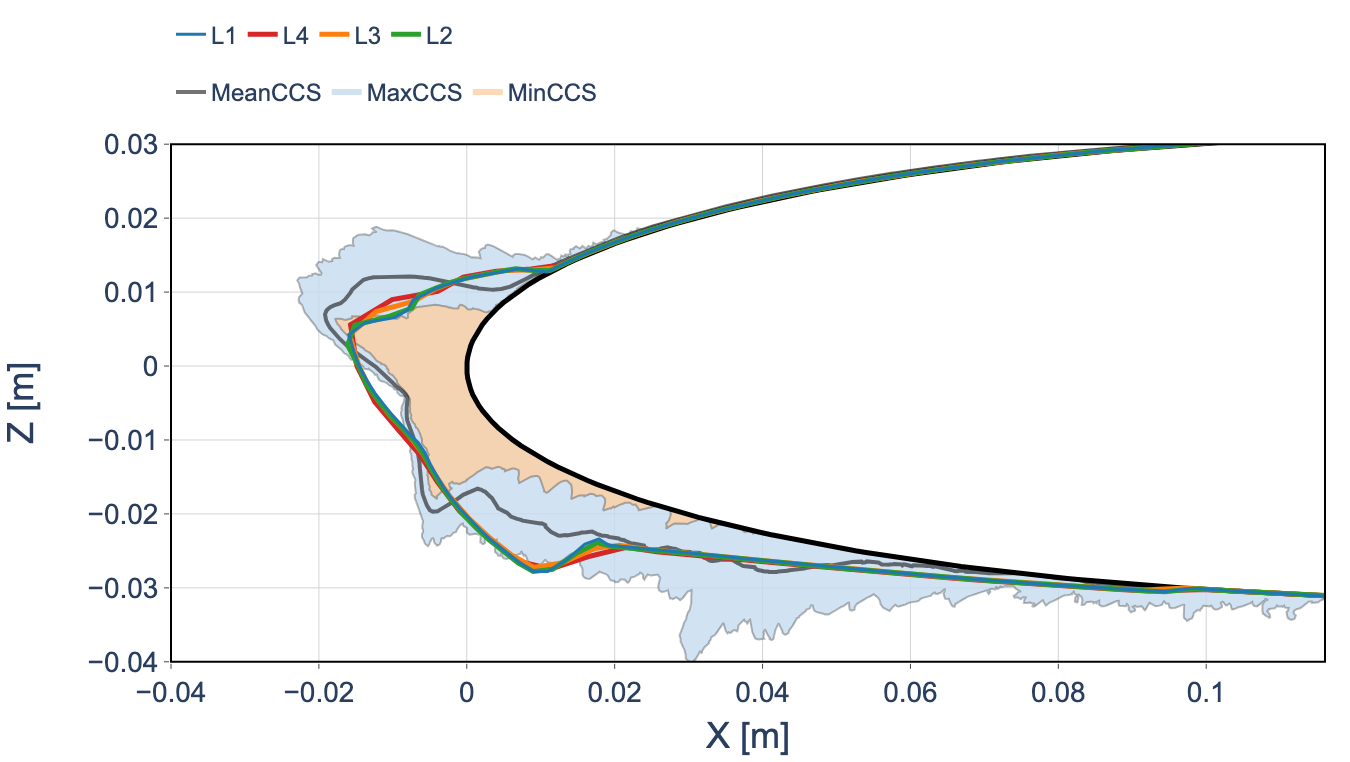
\includegraphics[
        width=\textwidth,
        trim={0cm 0cm 0cm 0.8cm},
        clip
    ]
    {FIGURES/NACA0012/ICE_SHAPES/tc_naca0012_ae3932_single_layer_ice_shape_slice_0p9144_bins15.png}
\end{column}

% ------------------------------------------------------------
% AE3933
% ------------------------------------------------------------
\begin{column}{0.50\textwidth}
    \centering
    \textbf{AE3933 - $K_s= 0.5334mm$}

    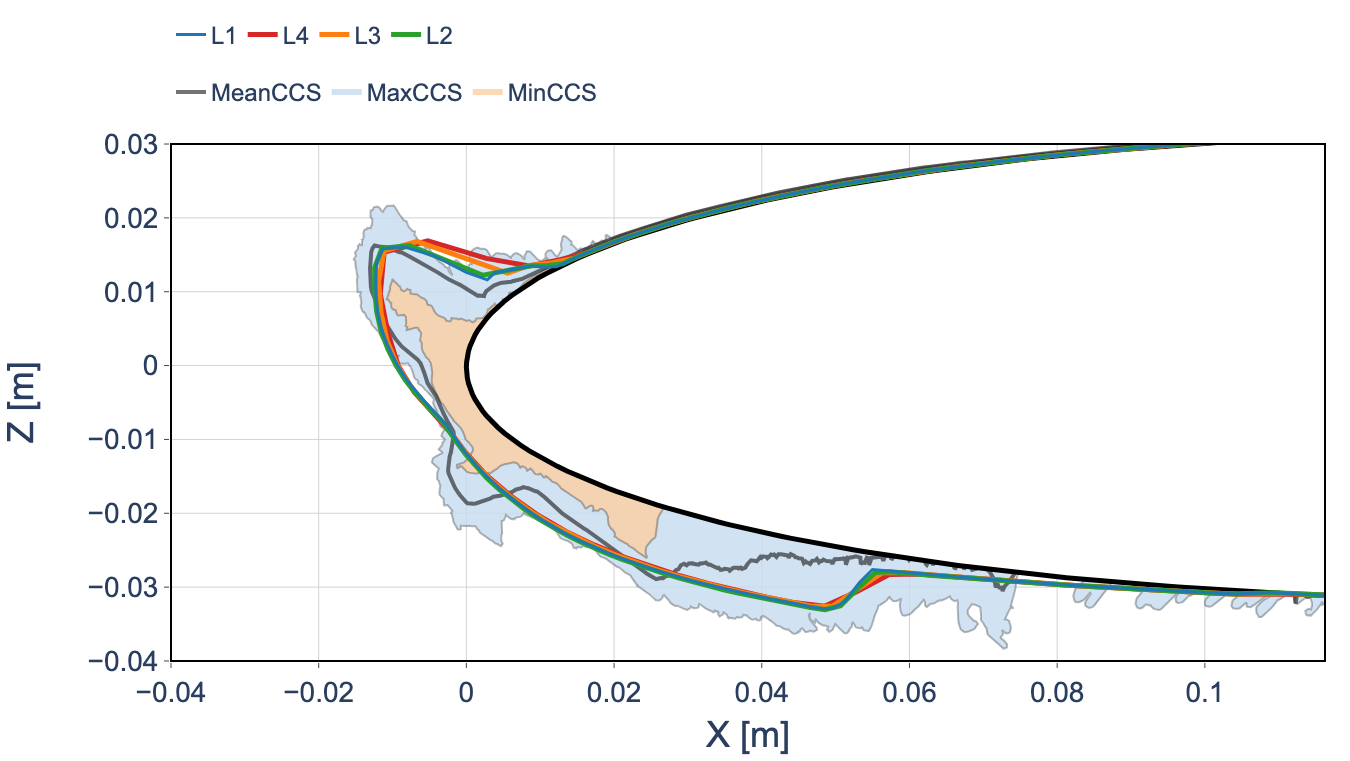
\includegraphics[
        width=\textwidth,
        trim={0cm 0cm 0cm 0.8cm},
        clip
    ]
    {FIGURES/NACA0012/ICE_SHAPES/tc_naca0012_ae3933_single_layer_ice_shape_slice_0p9144_bins15.png}
\end{column}

\end{columns}

\vspace{-0.10cm}

\begin{block}{\scriptsize Single-Layer Ice Shapes Assessment}
\begin{itemize}
    \item CHAMPS predicts consistent ice shapes across the grid hierarchy, with limited sensitivity to spatial refinement.
    \item Predictions remain largely within the experimental ice-shape envelope, with the main differences concentrated around the horn regions.
    \item Unlike the ice mass, the ice shape captures the effect of the warmer AE3933 condition, with a clear change in upper-horn orientation.
\end{itemize}
\end{block}

\end{frame}


% ============================================================
% NACA0012 -- 3D Ice Shapes
% ============================================================

\begin{frame}{\small NACA0012 -- Multilayer Ice Shapes}
\scriptsize

\vspace{-0.15cm}

\centering

% ------------------------------------------------------------
% AE3932
% ------------------------------------------------------------
\begin{minipage}[t]{0.40\textwidth}
    \centering
    \textbf{AE3932 - $K_s= 0.2667mm$}

    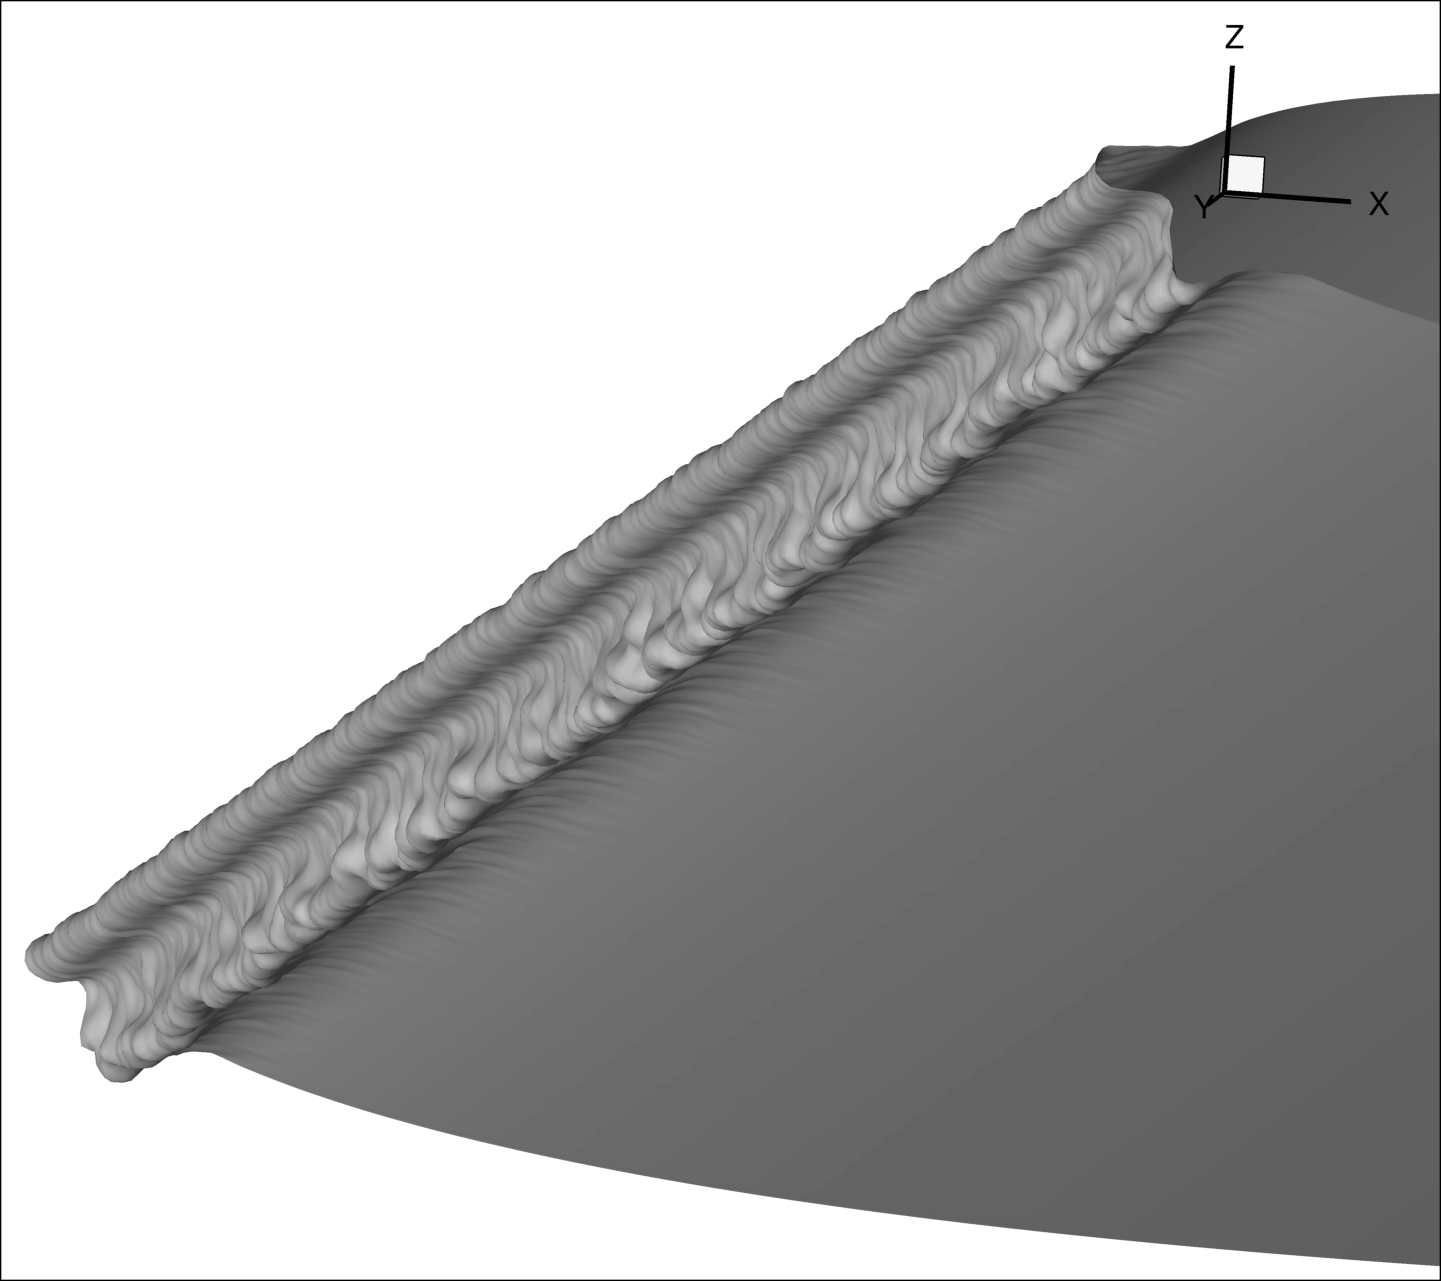
\includegraphics[
        width=\textwidth
    ]
    {FIGURES/NACA0012/ICE_VIEWS/NACA0012_AE3932.png}
\end{minipage}%
\hspace{1cm}
% ------------------------------------------------------------
% AE3933
% ------------------------------------------------------------
\begin{minipage}[t]{0.40\textwidth}
    \centering
    \textbf{AE3933 - $K_s= 0.2667mm$}

    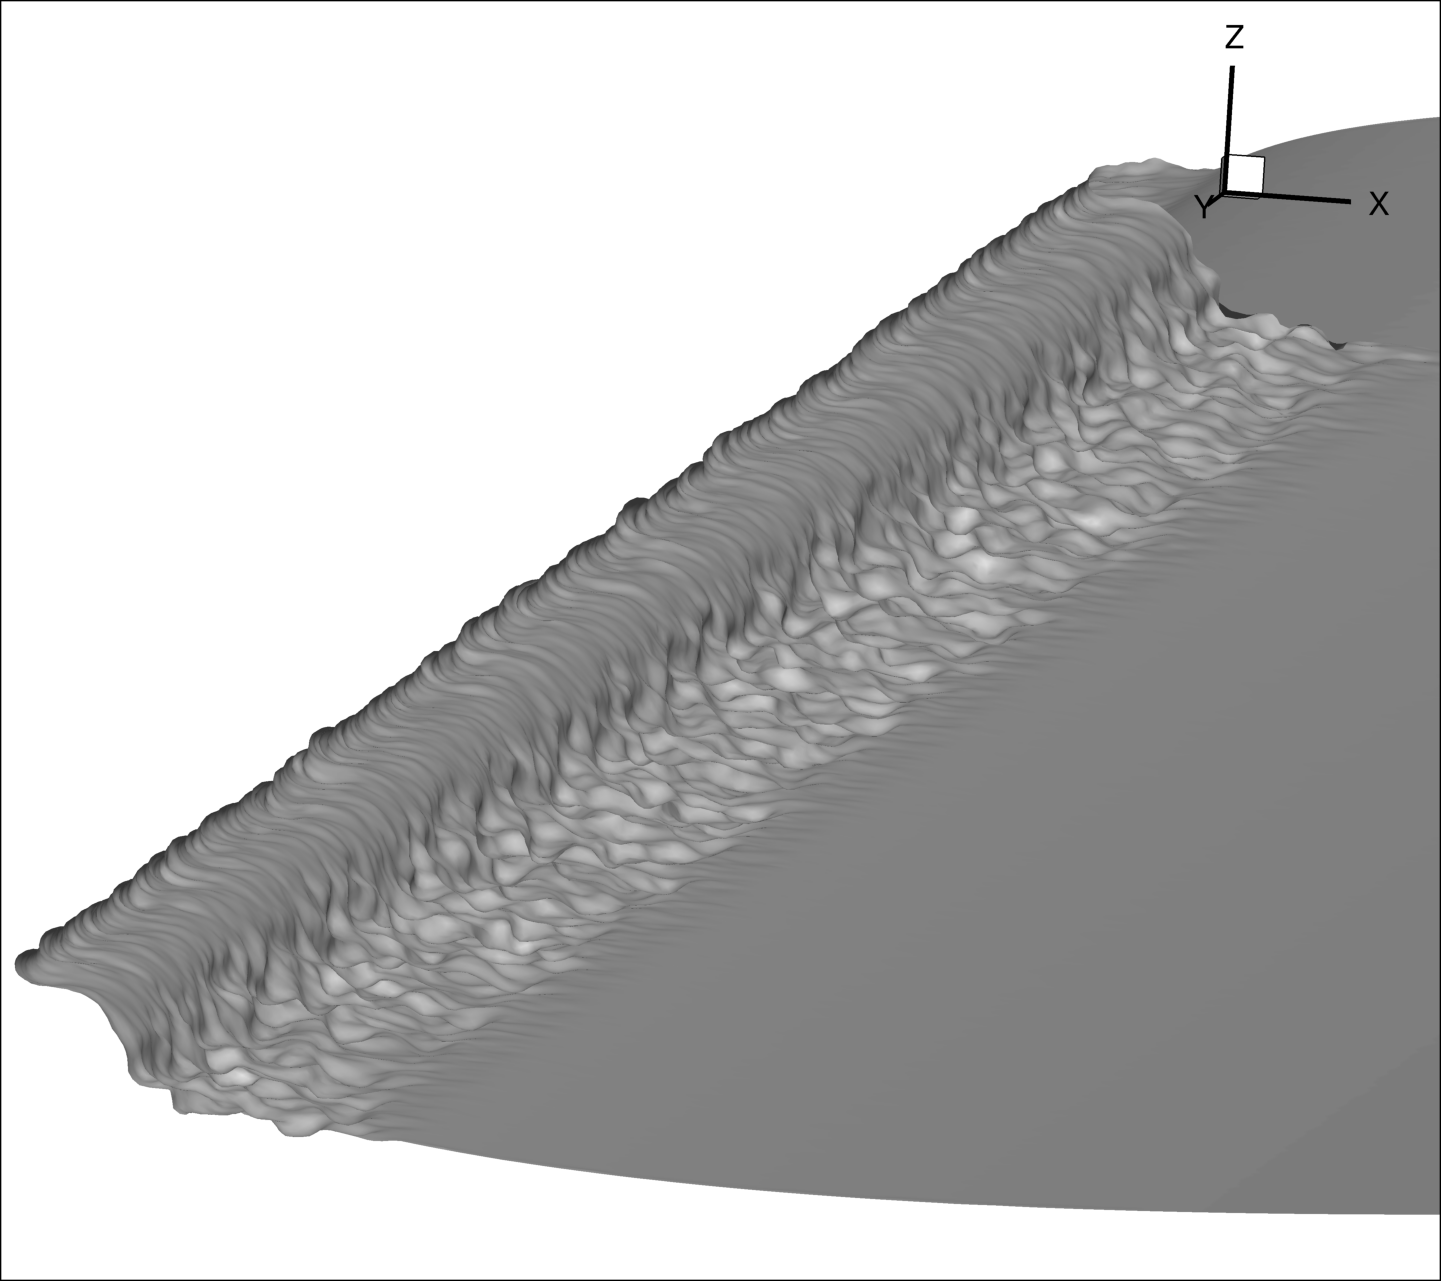
\includegraphics[
        width=\textwidth
    ]
    {FIGURES/NACA0012/ICE_VIEWS/NACA0012_AE3933.png}
\end{minipage}

\vspace{-0.10cm}

\begin{block}{\scriptsize Multilayer Ice Shapes Assessment}
\begin{itemize}
    \item The multilayer simulations capture the spanwise development of the ice horns.
    \item Distinct three-dimensional ice morphologies are obtained for the two icing conditions, consistent with the differences observed in the two-dimensional cross-sections.
\end{itemize}
\end{block}

\end{frame}


% ============================================================
% NACA0012 -- Multilayer Ice Shapes
% ============================================================

\begin{frame}{\small NACA0012 -- Multilayer Ice Shapes: Roughness Sensitivity}
\scriptsize

\vspace{-0.15cm}

\begin{columns}[T,onlytextwidth]

% ------------------------------------------------------------
% AE3932
% ------------------------------------------------------------
\begin{column}{0.50\textwidth}
    \centering
    \textbf{AE3932}

    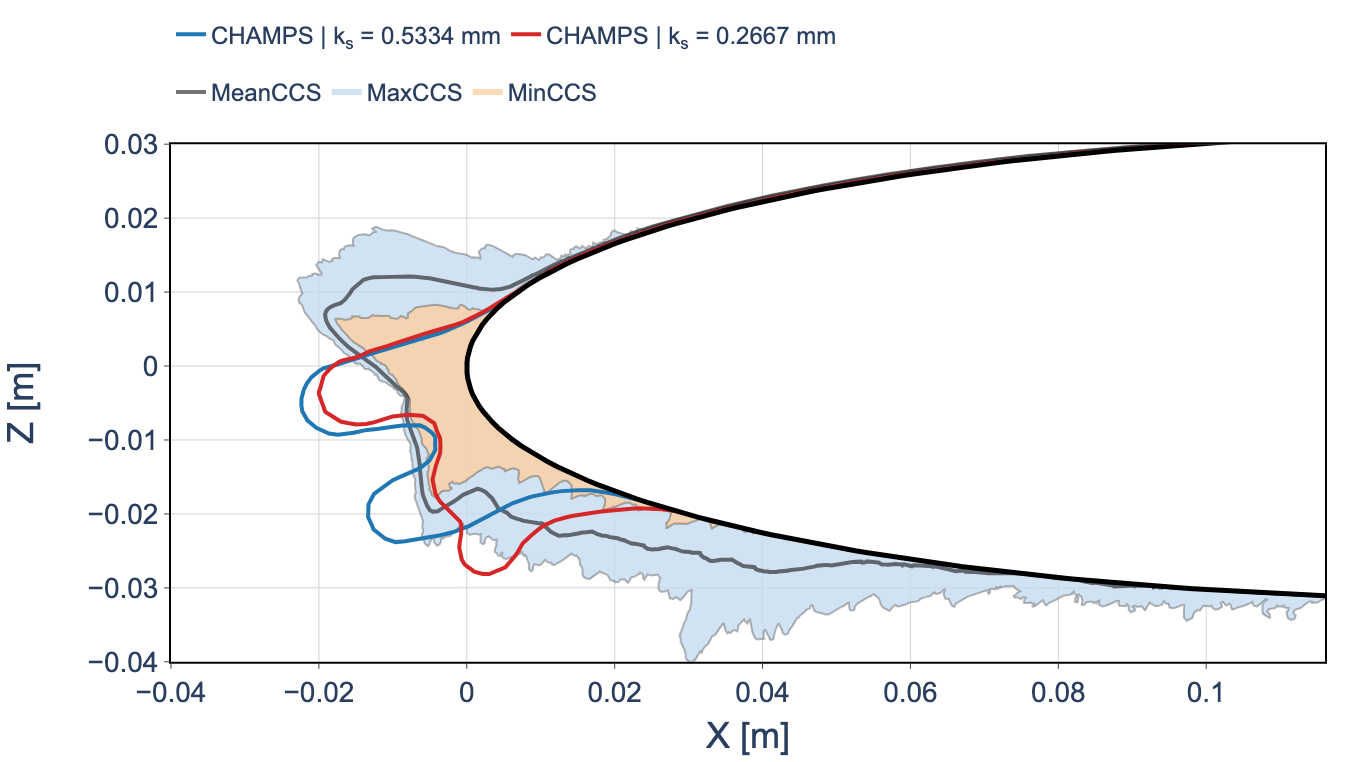
\includegraphics[
        width=\textwidth,
        trim={0cm 0cm 1cm 0.8cm},
        clip
    ]
    {FIGURES/NACA0012/ICE_SHAPES/tc_naca0012_ae3932_L1_multilayer_ice_shape_slice_0p9144_bins07_roughness_comparison.png}
\end{column}

% ------------------------------------------------------------
% AE3933
% ------------------------------------------------------------
\begin{column}{0.50\textwidth}
    \centering
    \textbf{AE3933}

    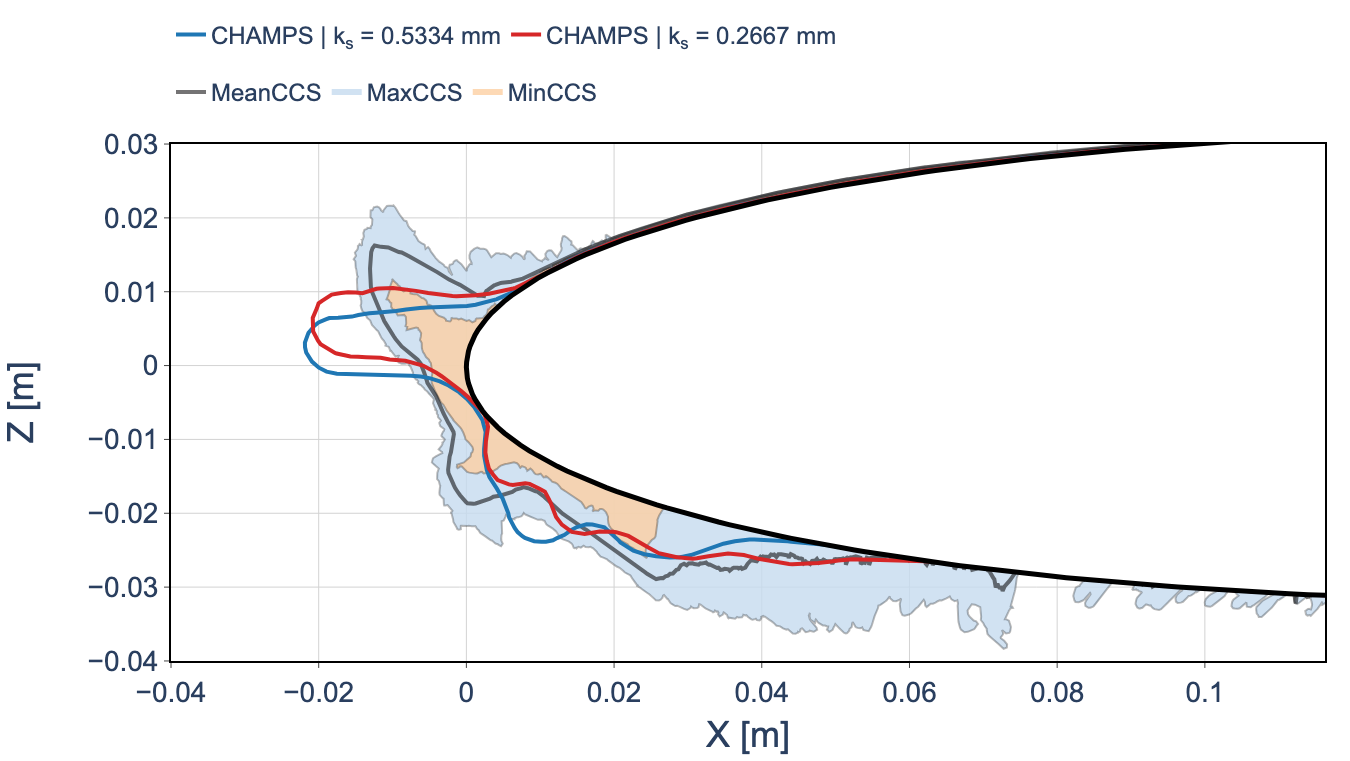
\includegraphics[
        width=\textwidth,
        trim={0cm 0cm 1cm 0.8cm},
        clip
    ]
    {FIGURES/NACA0012/ICE_SHAPES/tc_naca0012_ae3933_L1_multilayer_ice_shape_slice_0p9144_bins07_roughness_comparison.png}
\end{column}

\end{columns}

\vspace{-0.10cm}

\begin{block}{\scriptsize Multilayer Ice Shapes Assessment}
\begin{itemize}
    \item Surface roughness has a pronounced influence on the multilayer ice shapes, particularly on horn development.
    
    \item The lower roughness height provides better overall agreement with the experimental cross sections, but still underpredicts the upper-horn angle.
    
    \item The present simulations assume a constant roughness height and constant ice density, which influences the predicted location and development of the horns. Future work will investigate more advanced roughness and ice-density models for these cases.
\end{itemize}
\end{block}

\end{frame}
\section[ONERAM6]{\textbf{ONERAM6 Icing Results}}

% ============================================================
% ONERA M6 -- ICING RESULTS
% ============================================================

\begin{frame}[plain]
    \centering
    \vfill

    {\LARGE\bfseries ONERA M6 RESULTS}

    \vfill
\end{frame}

% ============================================================
% ONERA M6 -- Integrated Aerodynamic Coefficients
% ============================================================

\begin{frame}{\small ONERA M6 -- Integrated Aerodynamic Coefficients}
\scriptsize

\vspace{-0.20cm}

\begin{columns}[T,onlytextwidth]

% ------------------------------------------------------------
% CL
% ------------------------------------------------------------
\begin{column}{0.33\textwidth}
    \centering
    \textbf{$C_L$}

    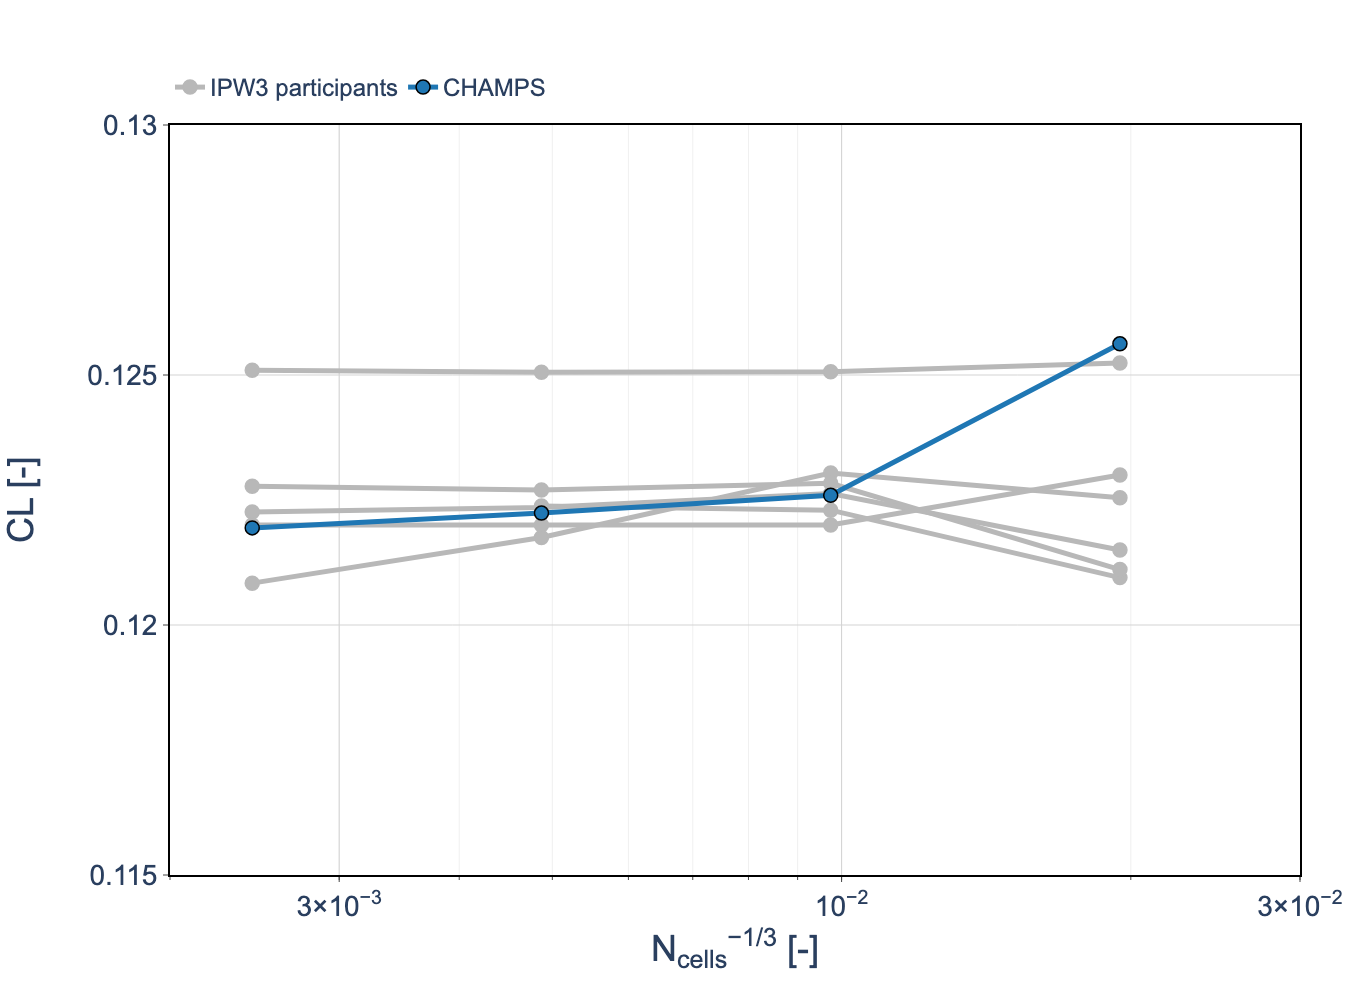
\includegraphics[
        width=\textwidth,
        trim={0cm 0cm 1cm 3.6cm},
        clip
    ]
    {FIGURES/ONERAM6/AERODYNAMIC/tc_oneram6_cl_vs_n_1mm.png}
\end{column}

% ------------------------------------------------------------
% CD
% ------------------------------------------------------------
\begin{column}{0.33\textwidth}
    \centering
    \textbf{$C_D$}

    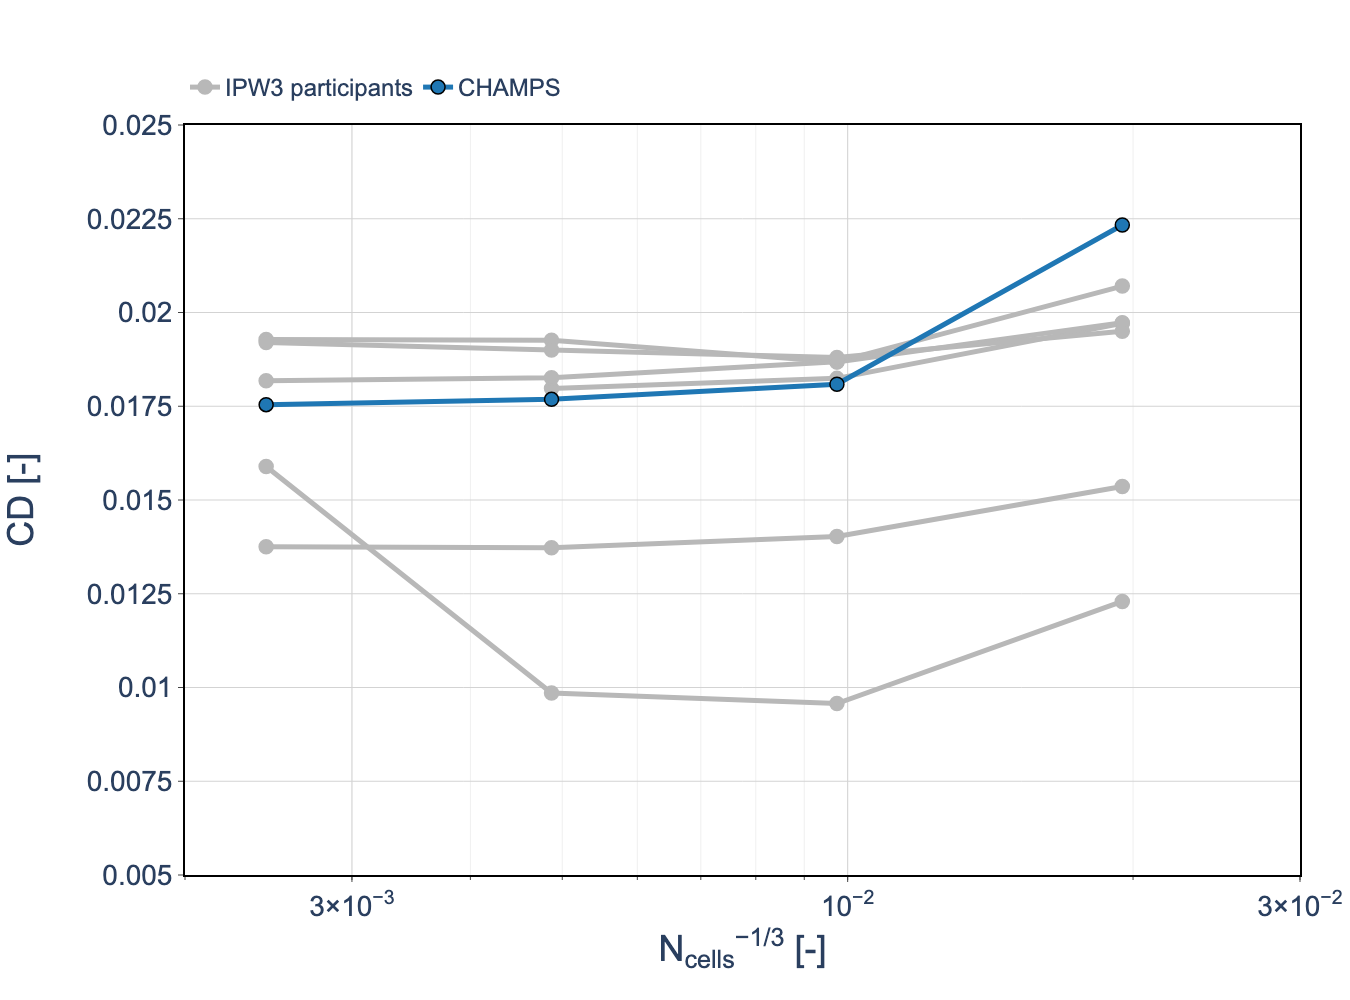
\includegraphics[
        width=\textwidth,
        trim={0cm 0cm 1cm 3.6cm},
        clip
    ]
    {FIGURES/ONERAM6/AERODYNAMIC/tc_oneram6_cd_vs_n_1mm.png}
\end{column}

% ------------------------------------------------------------
% CMY
% ------------------------------------------------------------
\begin{column}{0.33\textwidth}
    \centering
    \textbf{$C_{MY}$}

    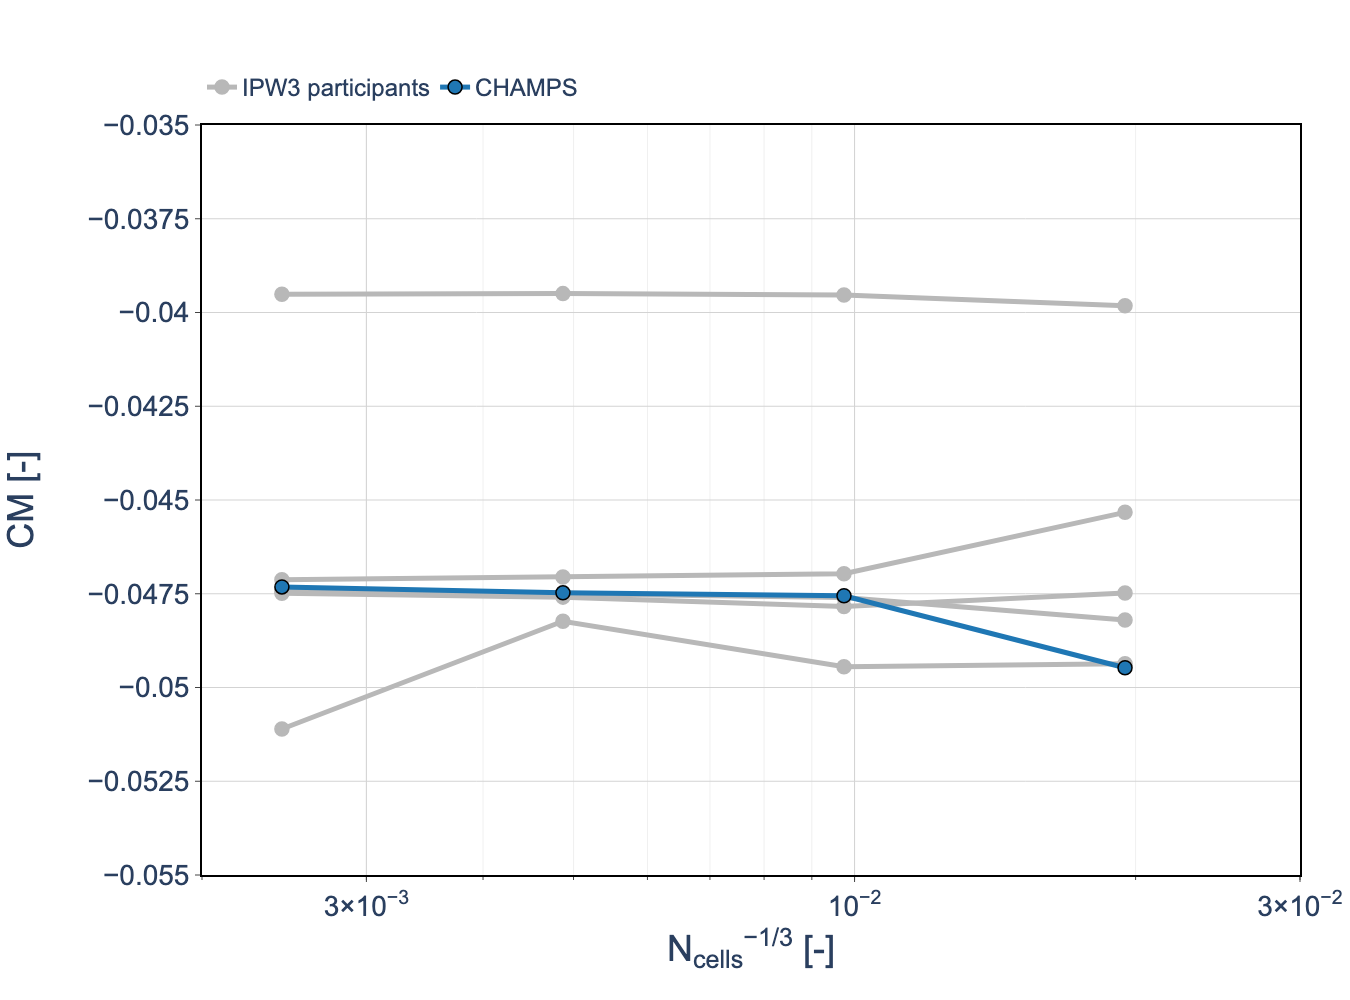
\includegraphics[
        width=\textwidth,
        trim={0cm 0cm 1cm 3.6cm},
        clip
    ]
    {FIGURES/ONERAM6/AERODYNAMIC/tc_oneram6_cmy_vs_n_1mm.png}
\end{column}

\end{columns}

\vspace{-0.10cm}

\begin{center}
\renewcommand{\arraystretch}{1.20}
\setlength{\tabcolsep}{6pt}

\begin{tabular}{lccc}
\toprule
& $\mathbf{C_L}$ & $\mathbf{C_D}$ & $\mathbf{C_{MY}}$ \\
\midrule

\textbf{CHAMPS}
& 0.12194
& 0.01754
& -0.04732 \\

\textbf{IPW3 L1 Median}
& 0.12213
& 0.01786
& -0.04736 \\

\textbf{Difference}
& -0.15\%
& -1.78\%
& -0.09\% \\

\bottomrule
\end{tabular}
\end{center}

\vspace{-0.15cm}

\begin{block}{\scriptsize Integrated Aerodynamic Coefficients Assessment}
CHAMPS predicts the L1 integrated aerodynamic coefficients very close to the
IPW3 medians, with differences below 2\% for all three coefficients.
Limited grid sensitivity is observed on the three finest grids, while the
coarsest L4 grid produces a more noticeable deviation, particularly for $C_D$.
\end{block}

\end{frame}

% ============================================================
% ONERA M6 -- Pressure-Coefficient Distributions
% ============================================================

\begin{frame}{\small ONERA M6 -- Pressure-Coefficient Distributions}
\scriptsize

\vspace{-0.20cm}

\begin{columns}[T,onlytextwidth]

% ------------------------------------------------------------
% y = 0.10 m
% ------------------------------------------------------------
\begin{column}{0.33\textwidth}
    \centering
    \textbf{$y=0.10$ m}

    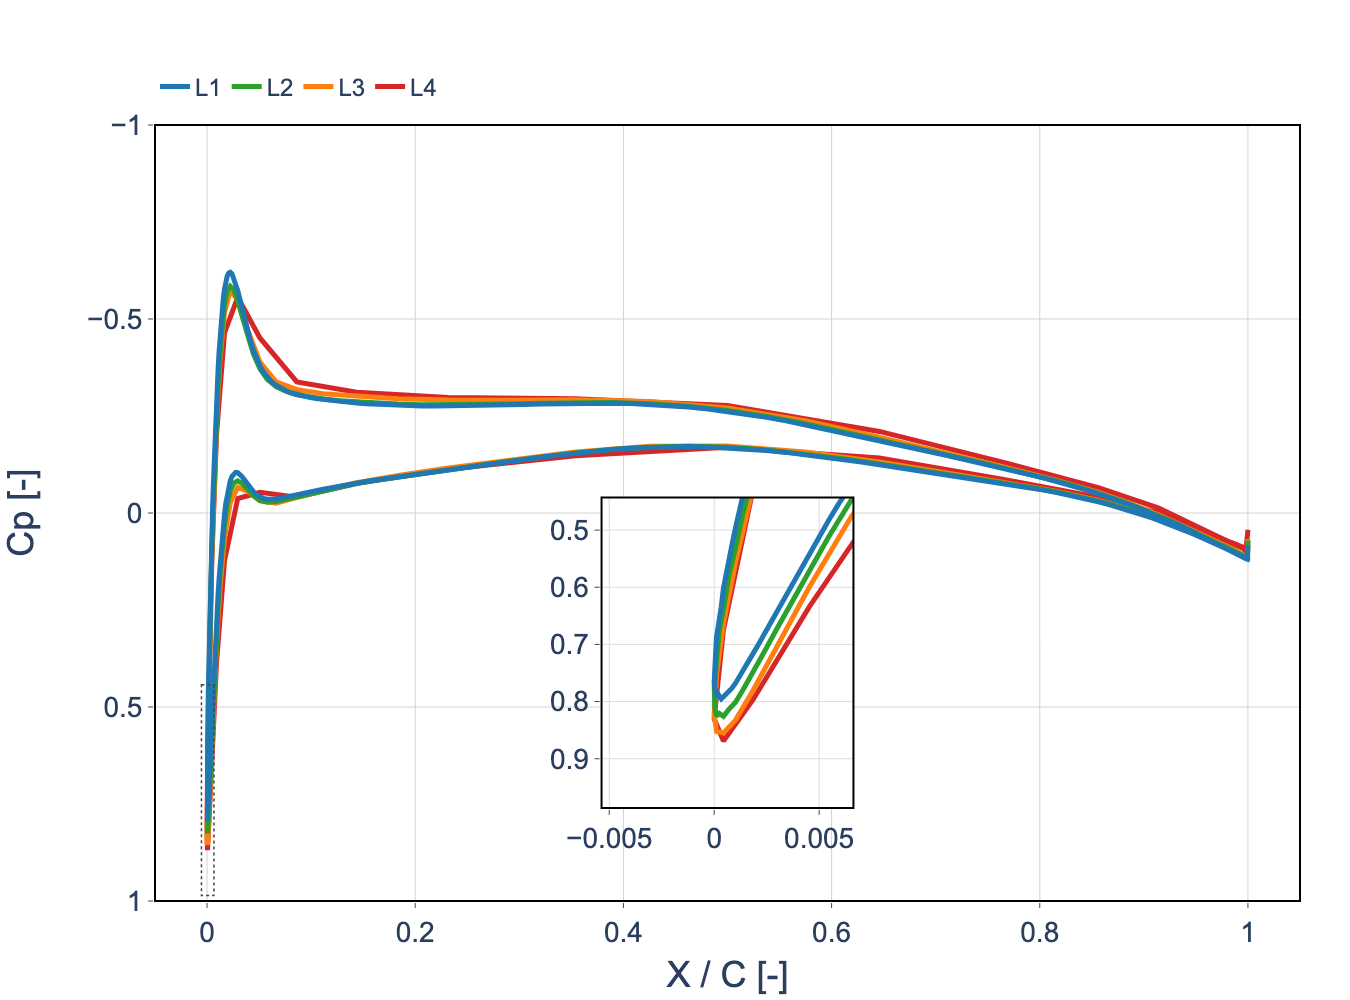
\includegraphics[
        width=\textwidth,
        trim={0cm 0cm 1cm 1.2cm},
        clip
    ]
    {FIGURES/ONERAM6/AERODYNAMIC/tc_oneram6_L1_cp_vs_x_slice_0p1_roughness_1mm.png}
\end{column}

% ------------------------------------------------------------
% y = 0.75 m
% ------------------------------------------------------------
\begin{column}{0.33\textwidth}
    \centering
    \textbf{$y=0.75$ m}

    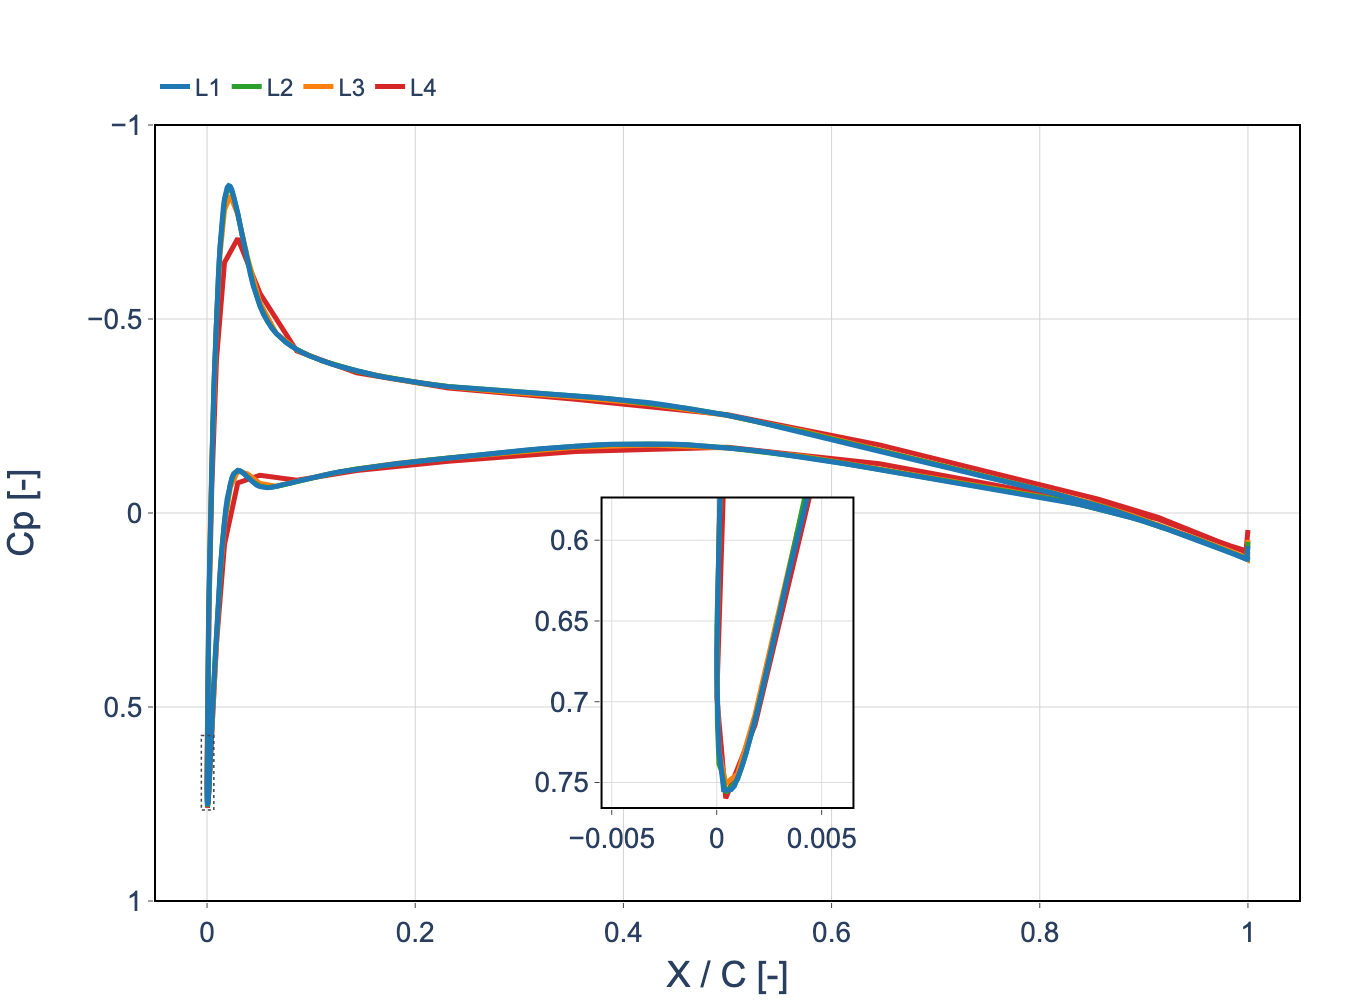
\includegraphics[
        width=\textwidth,
        trim={0cm 0cm 1cm 1.2cm},
        clip
    ]
    {FIGURES/ONERAM6/AERODYNAMIC/tc_oneram6_L1_cp_vs_x_slice_0p75_roughness_1mm.png}
\end{column}

% ------------------------------------------------------------
% y = 1.40 m
% ------------------------------------------------------------
\begin{column}{0.33\textwidth}
    \centering
    \textbf{$y=1.40$ m}

    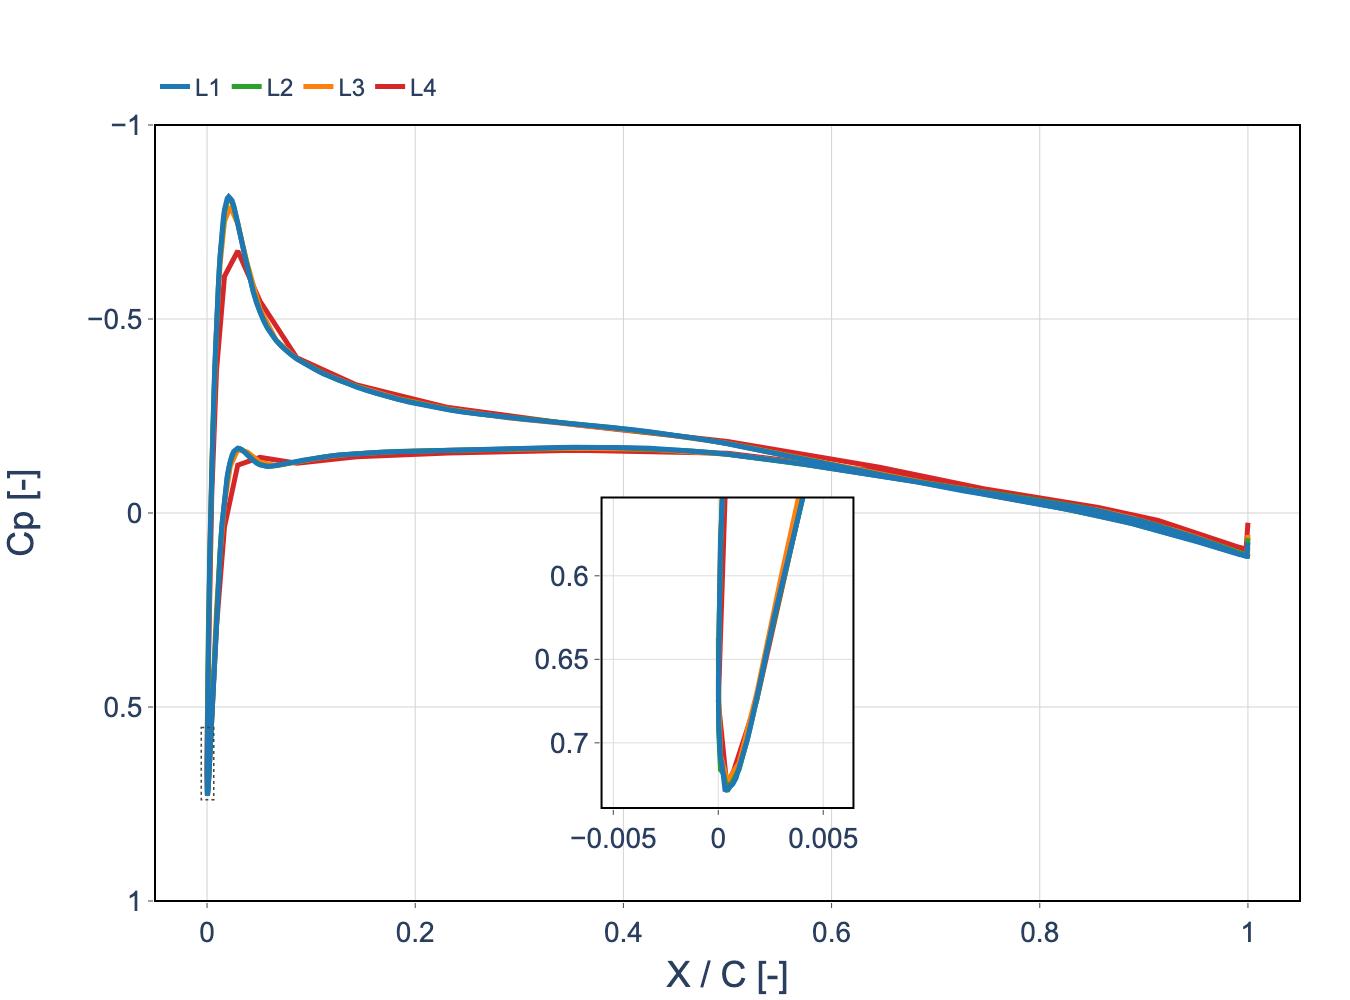
\includegraphics[
        width=\textwidth,
        trim={0cm 0cm 1cm 1.2cm},
        clip
    ]
    {FIGURES/ONERAM6/AERODYNAMIC/tc_oneram6_L1_cp_vs_x_slice_1p4_roughness_1mm.png}
\end{column}

\end{columns}

\vspace{-0.05cm}

\begin{block}{\scriptsize Pressure-Coefficient Assessment}
CHAMPS pressure distributions are consistent across the grid hierarchy at all three spanwise stations, with L4 exhibiting the largest deviations.
\end{block}

\end{frame}

% ============================================================
% ONERA M6 -- Droplet Impingement: Eulerian vs Lagrangian
% ============================================================

\begin{frame}{\small ONERA M6 -- Droplet Collection Efficiency (L1, 1 Bin -- Eulerian vs Lagrangian)}
\scriptsize

\vspace{-0.20cm}

\begin{columns}[T,onlytextwidth]

% ------------------------------------------------------------
% y = 0.10 m
% ------------------------------------------------------------
\begin{column}{0.33\textwidth}
    \centering
    \textbf{$y=0.10$ m}

    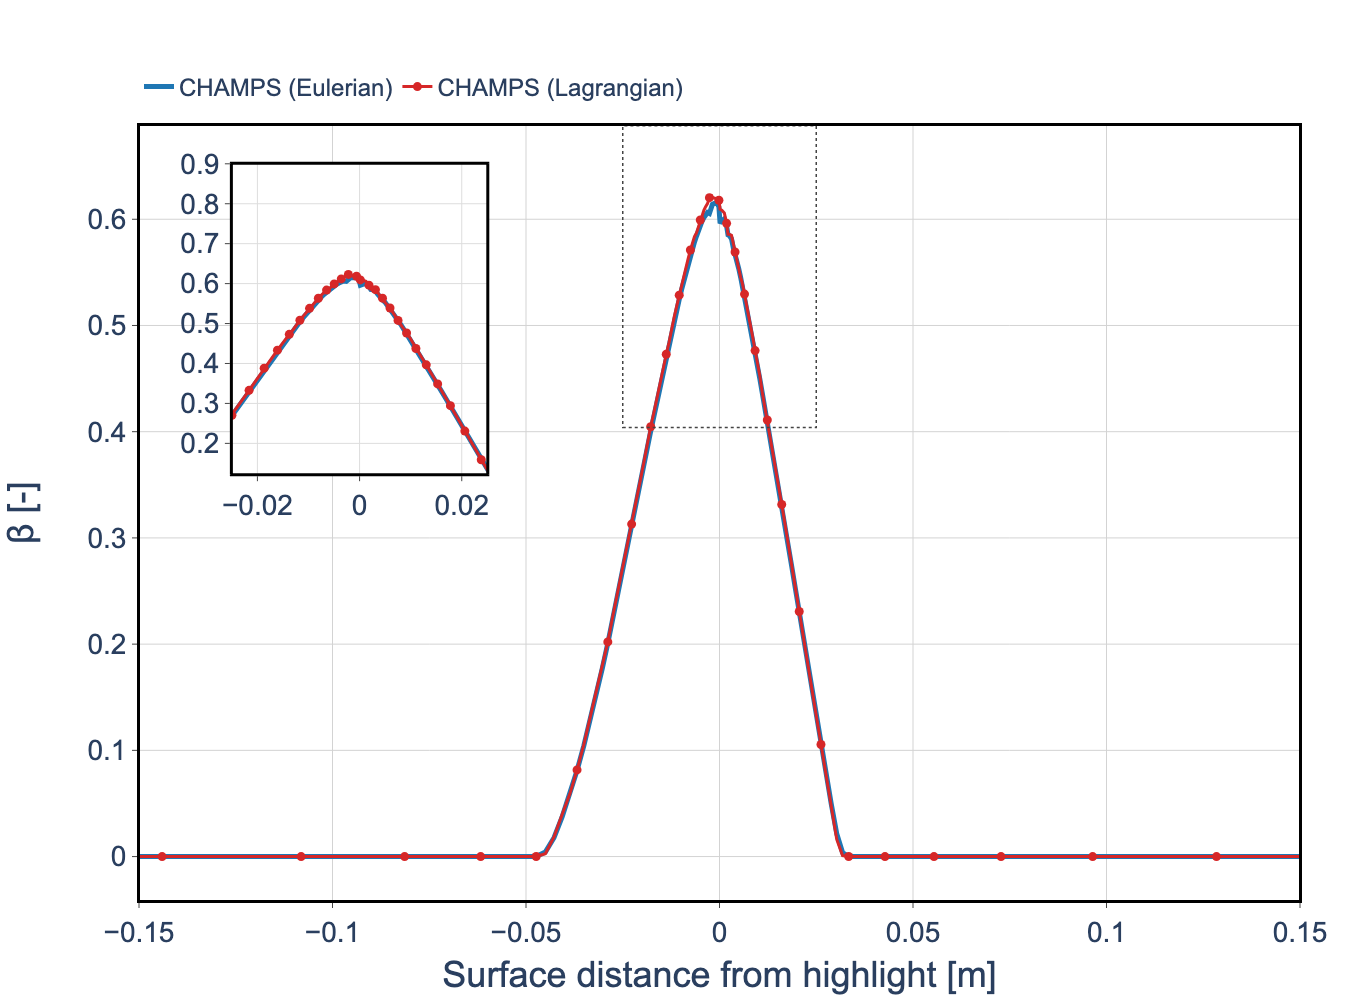
\includegraphics[
        width=\textwidth,
        trim={0cm 0cm 1cm 1.2cm},
        clip
    ]
    {FIGURES/ONERAM6/IMPINGEMENT/tc_oneram6_L1_beta_bins01_vs_s_slice_0p1_roughness_1mm.png}
\end{column}

% ------------------------------------------------------------
% y = 0.75 m
% ------------------------------------------------------------
\begin{column}{0.33\textwidth}
    \centering
    \textbf{$y=0.75$ m}

    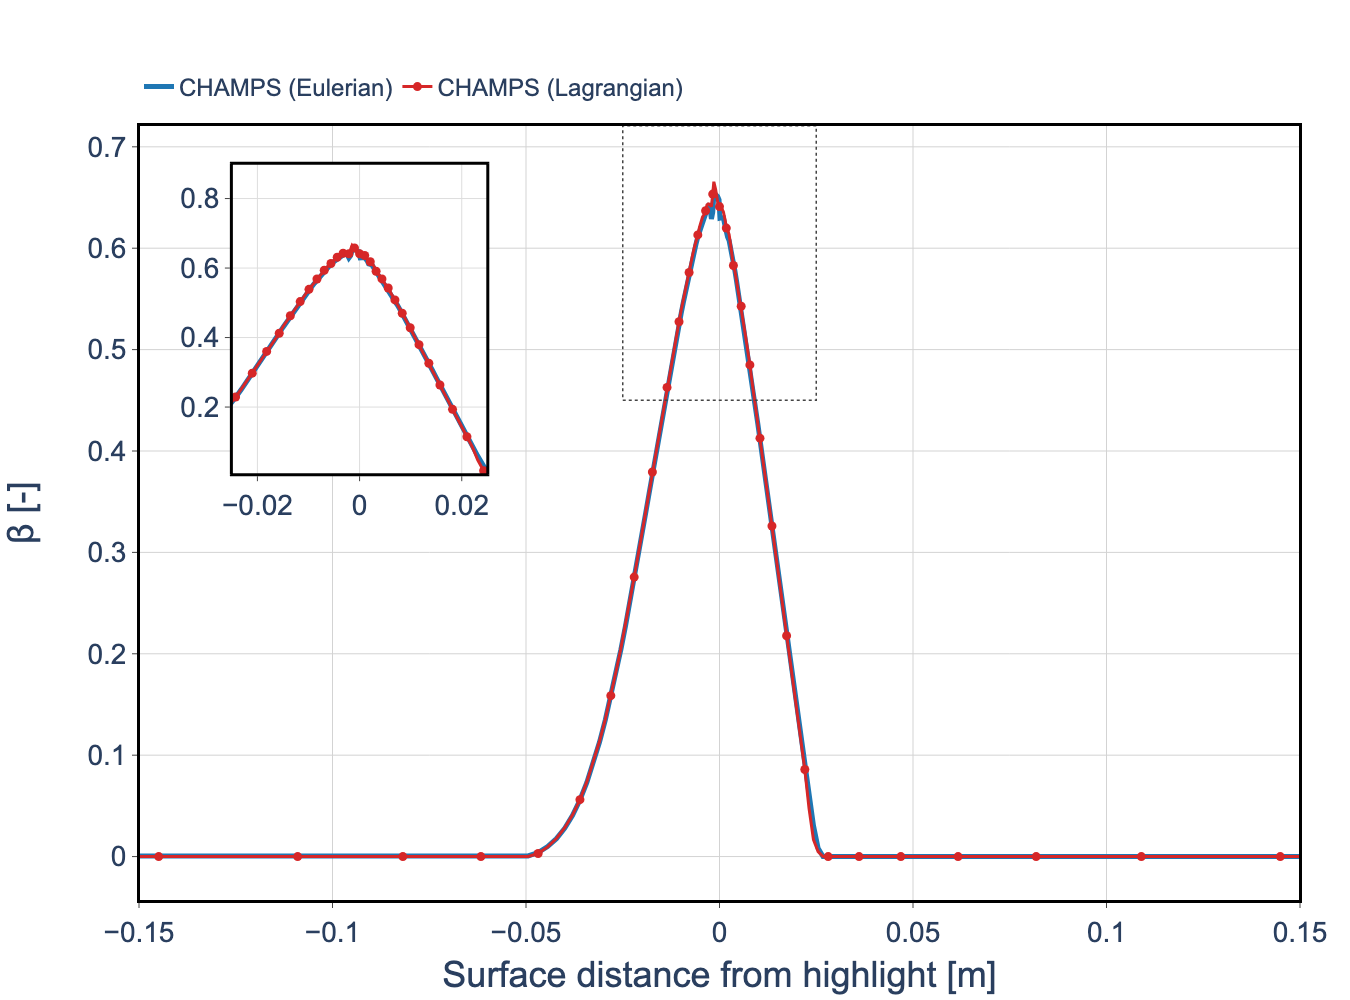
\includegraphics[
        width=\textwidth,
        trim={0cm 0cm 1cm 1.2cm},
        clip
    ]
    {FIGURES/ONERAM6/IMPINGEMENT/tc_oneram6_L1_beta_bins01_vs_s_slice_0p75_roughness_1mm.png}
\end{column}

% ------------------------------------------------------------
% y = 1.40 m
% ------------------------------------------------------------
\begin{column}{0.33\textwidth}
    \centering
    \textbf{$y=1.40$ m}

    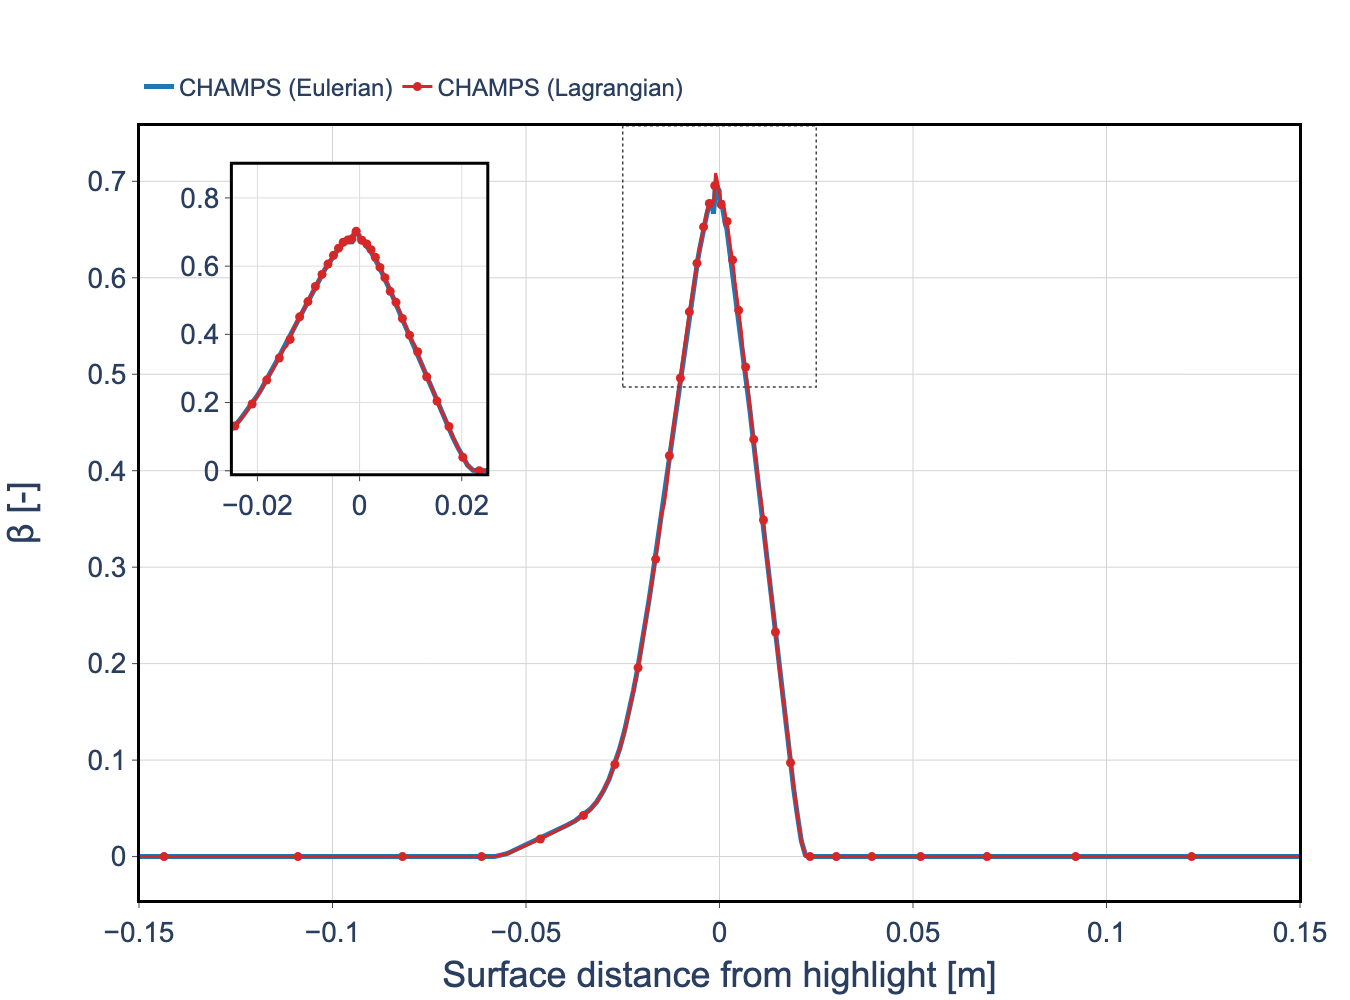
\includegraphics[
        width=\textwidth,
        trim={0cm 0cm 1cm 1.2cm},
        clip
    ]
    {FIGURES/ONERAM6/IMPINGEMENT/tc_oneram6_L1_beta_bins01_vs_s_slice_1p4_roughness_1mm.png}
\end{column}

\end{columns}

\vspace{-0.05cm}

\begin{block}{\scriptsize Impingement Assessment}
The Eulerian and Lagrangian CHAMPS formulations predict nearly identical
collection-efficiency distributions at all three spanwise stations, with
consistent peak collection efficiencies and impingement extents.
\end{block}

\end{frame}


% ============================================================
% ONERA M6 -- Droplet Impingement: Bin Refinement
% ============================================================

\begin{frame}{\small ONERA M6 -- Droplet-Bin Refinement (L1 -- Eulerian)}
\scriptsize

\vspace{-0.20cm}

\begin{columns}[T,onlytextwidth]

% ------------------------------------------------------------
% y = 0.10 m
% ------------------------------------------------------------
\begin{column}{0.33\textwidth}
    \centering
    \textbf{$y=0.10$ m}

    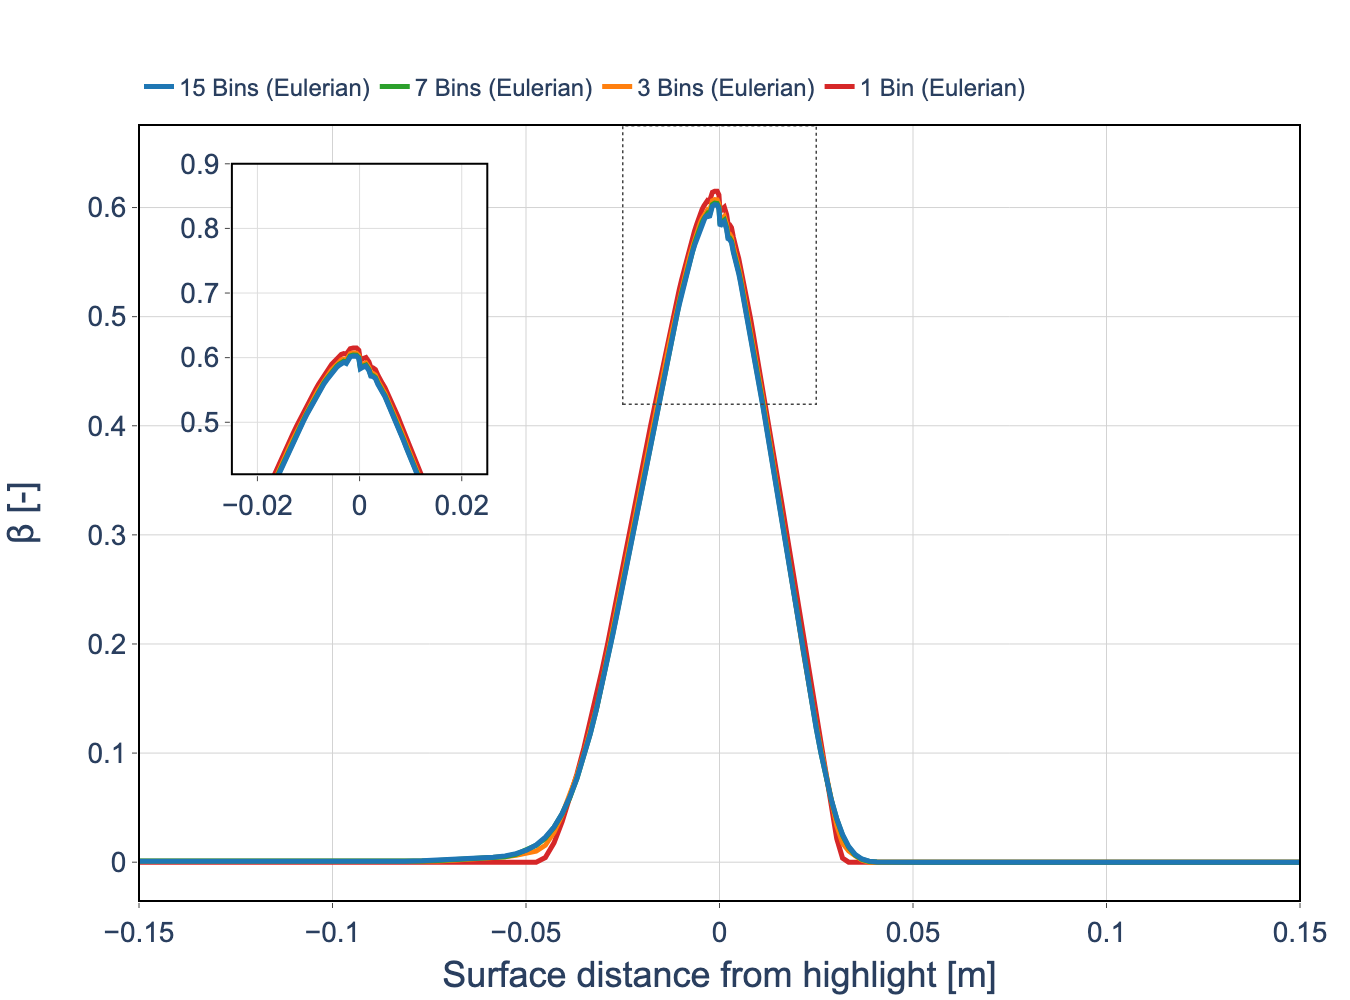
\includegraphics[
        width=\textwidth,
        trim={0cm 0cm 1cm 1.2cm},
        clip
    ]
    {FIGURES/ONERAM6/IMPINGEMENT/tc_oneram6_L1_beta_all_bins_vs_s_slice_0p1_roughness_1mm.png}
\end{column}

% ------------------------------------------------------------
% y = 0.75 m
% ------------------------------------------------------------
\begin{column}{0.33\textwidth}
    \centering
    \textbf{$y=0.75$ m}

    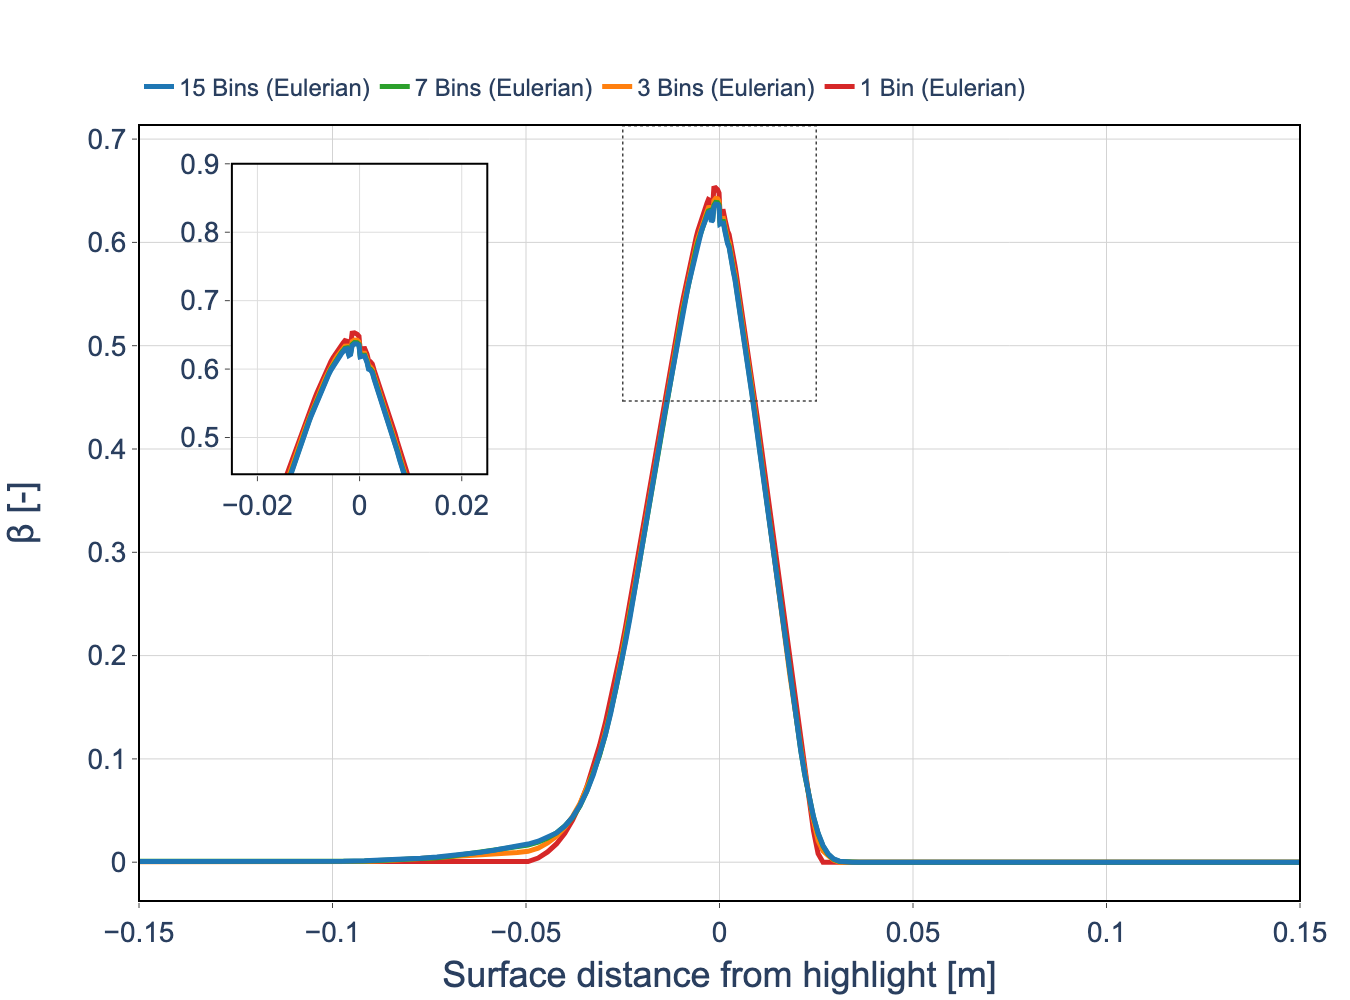
\includegraphics[
        width=\textwidth,
        trim={0cm 0cm 1cm 1.2cm},
        clip
    ]
    {FIGURES/ONERAM6/IMPINGEMENT/tc_oneram6_L1_beta_all_bins_vs_s_slice_0p75_roughness_1mm.png}
\end{column}

% ------------------------------------------------------------
% y = 1.40 m
% ------------------------------------------------------------
\begin{column}{0.33\textwidth}
    \centering
    \textbf{$y=1.40$ m}

    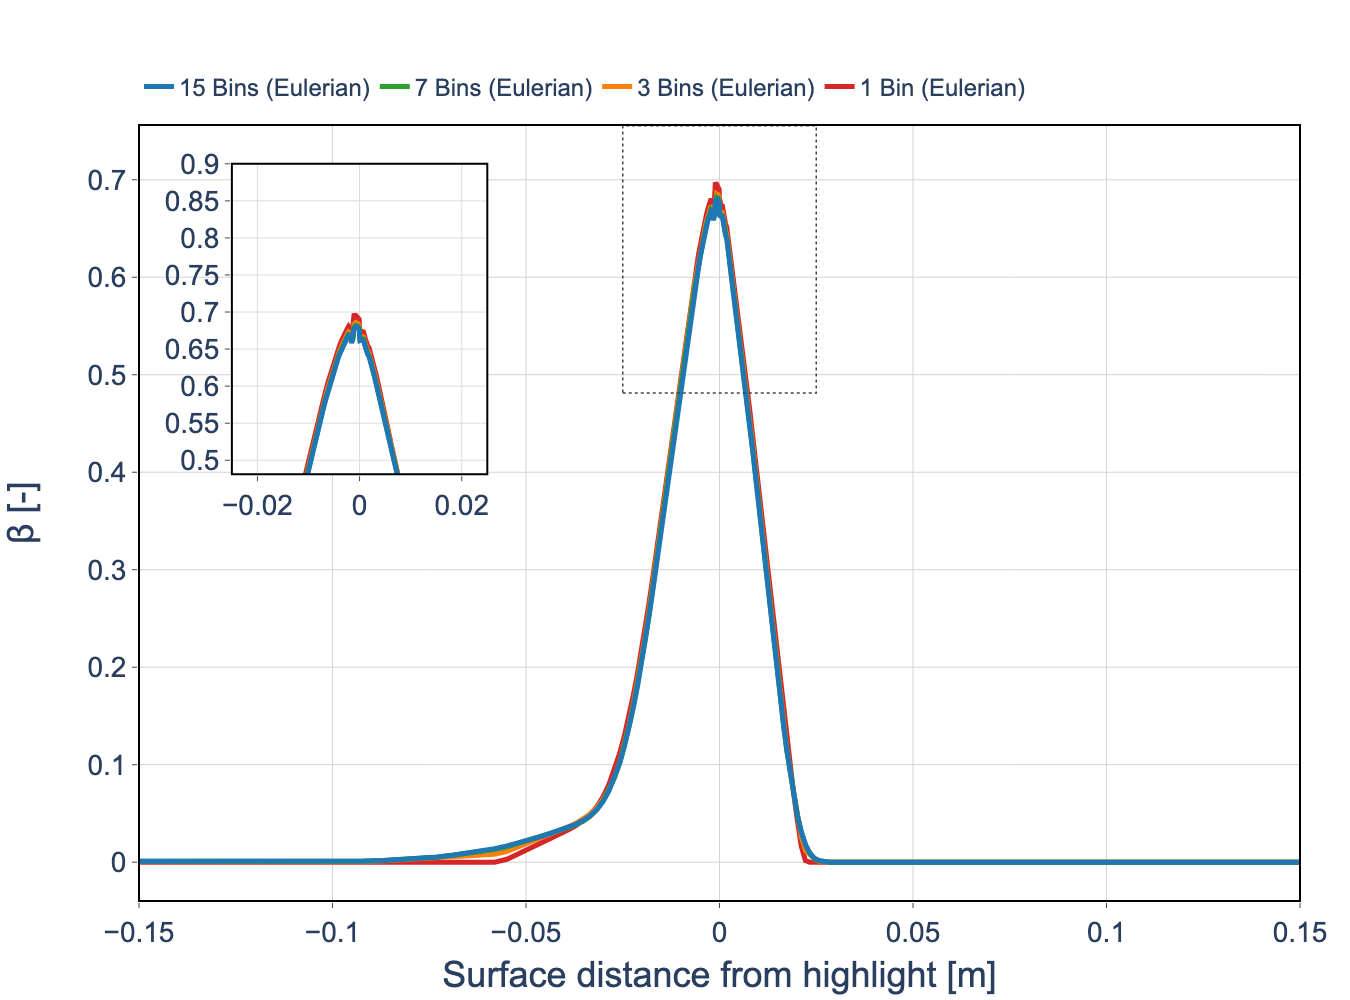
\includegraphics[
        width=\textwidth,
        trim={0cm 0cm 1cm 1.2cm},
        clip
    ]
    {FIGURES/ONERAM6/IMPINGEMENT/tc_oneram6_L1_beta_all_bins_vs_s_slice_1p4_roughness_1mm.png}
\end{column}

\end{columns}

\vspace{-0.05cm}

\begin{block}{\scriptsize Impingement Assessment}
\begin{itemize}
    \item Droplet-bin refinement has a limited influence on the collection-efficiency distributions at all three spanwise stations.
    \item Differences between the droplet distributions are less apparent than for the NACA0012 case, as the droplet-size distributions are more concentrated around the MVD.
    \item The remaining differences are primarily observed near the peak collection efficiency and at the impingement limits.
\end{itemize}
\end{block}

\end{frame}

% ============================================================
% ONERA M6 -- Ice Mass
% ============================================================

\begin{frame}{\small ONERA M6 -- Ice-Mass Prediction}
\scriptsize

\vspace{-0.20cm}

\begin{columns}[T,onlytextwidth]

% ------------------------------------------------------------
% Grid Refinement
% ------------------------------------------------------------
\begin{column}{0.50\textwidth}
    \centering
    \textbf{Grid Refinement -- 15 Bins}

    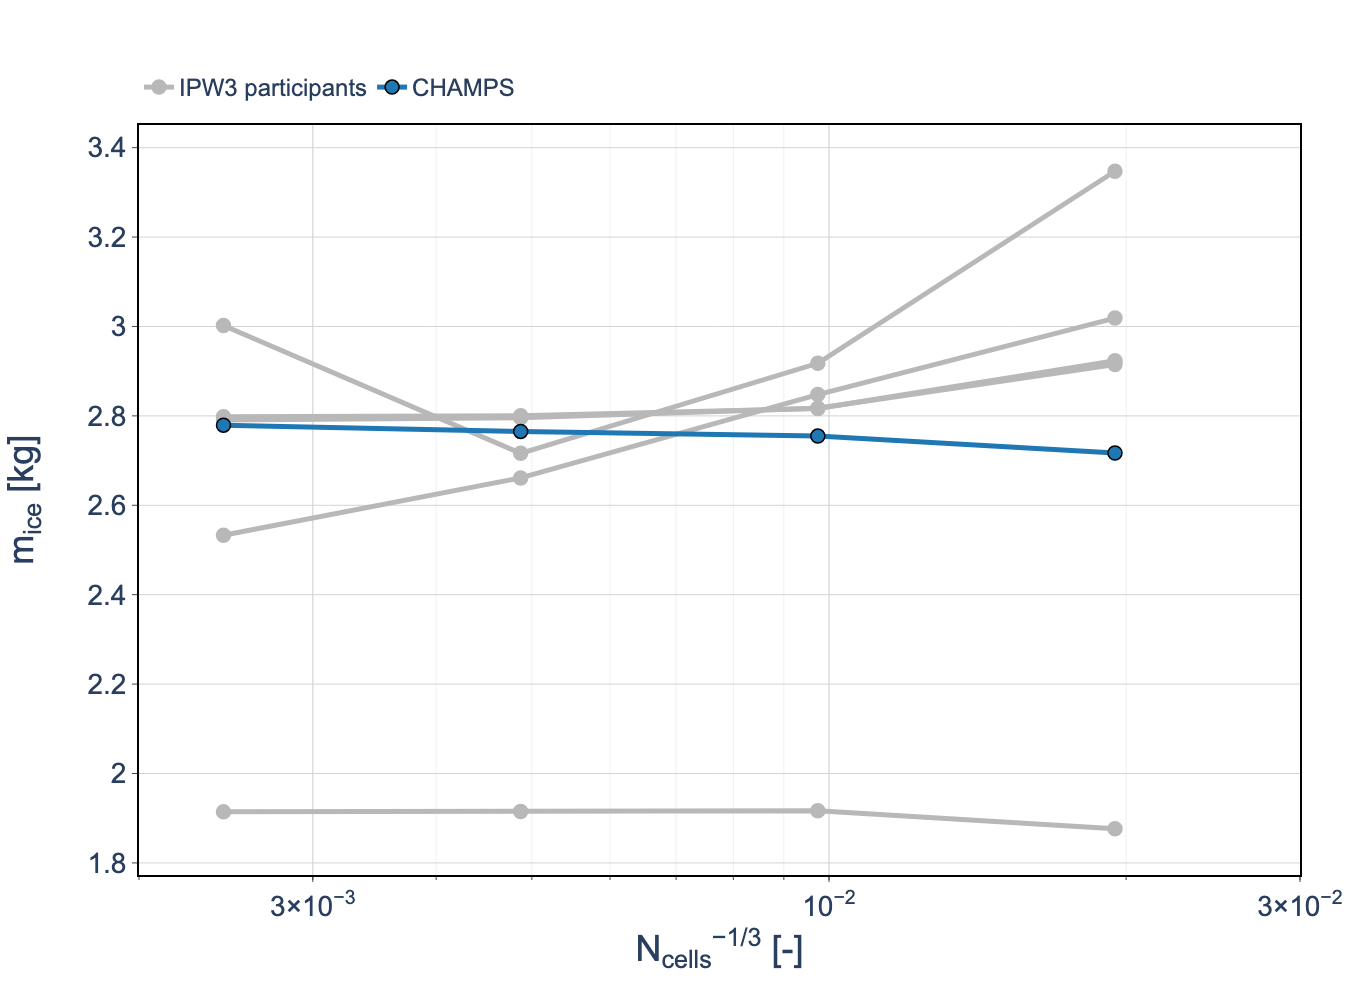
\includegraphics[
        width=\textwidth,
        trim={0cm 0cm 0cm 1.8cm},
        clip
    ]
    {FIGURES/ONERAM6/ICE_ACCRETION/tc_oneram6_ice_mass_vs_n_1mm_bins15_all_grid_levels.png}
\end{column}

% ------------------------------------------------------------
% Droplet-Bin Refinement
% ------------------------------------------------------------
\begin{column}{0.50\textwidth}
    \centering
    \textbf{Droplet-Bin Refinement -- L1}

    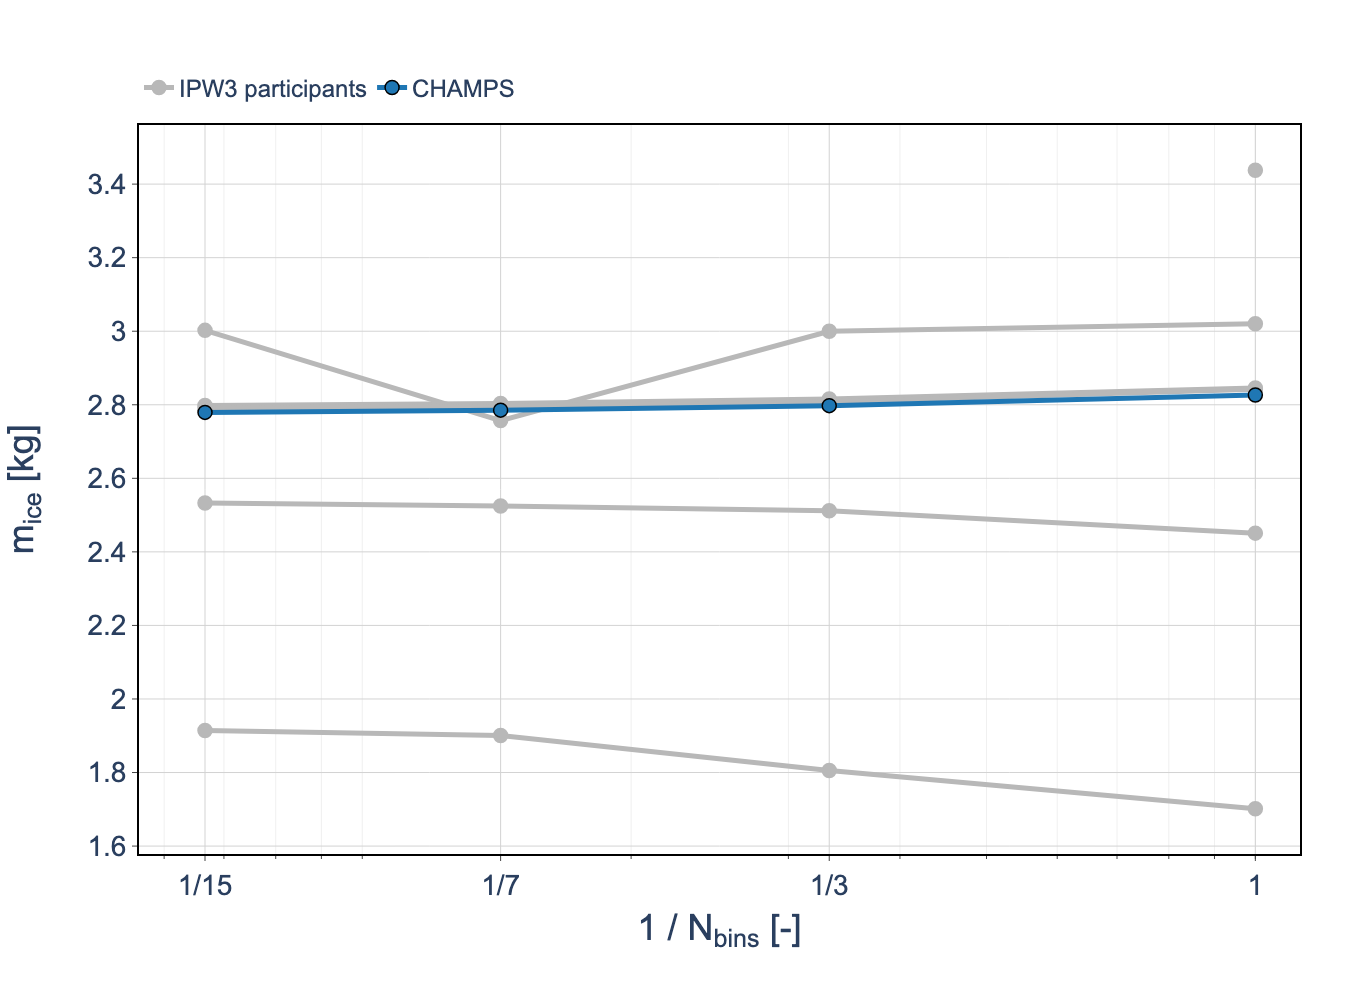
\includegraphics[
        width=\textwidth,
        trim={0cm 0cm 0cm 1.8cm},
        clip
    ]
    {FIGURES/ONERAM6/ICE_ACCRETION/tc_oneram6_ice_mass_vs_n_1mm_l1_vs_inverse_bins.png}
\end{column}

\end{columns}

\vspace{-0.10cm}

\begin{block}{\scriptsize Ice-Accretion Assessment}
\begin{itemize}
    \item CHAMPS predicts approximately $2.8$ kg of ice, with limited sensitivity to both spatial grid refinement and the number of droplet bins.
    \item Approximately $89\%$ of the impinging water mass is converted to ice; the remaining mass is predominantly lost through evaporation.
\end{itemize}
\end{block}

\end{frame}

% ============================================================
% ONERA M6 -- Single-Layer Ice Shapes
% ============================================================

\begin{frame}{\small ONERA M6 -- Single-Layer Ice-Shape Comparison}
\scriptsize

\vspace{-0.15cm}

\begin{columns}[T,onlytextwidth]

% ------------------------------------------------------------
% y = 0.10 m
% ------------------------------------------------------------
\begin{column}{0.333\textwidth}
    \centering
    \textbf{$y=0.10$ m}

    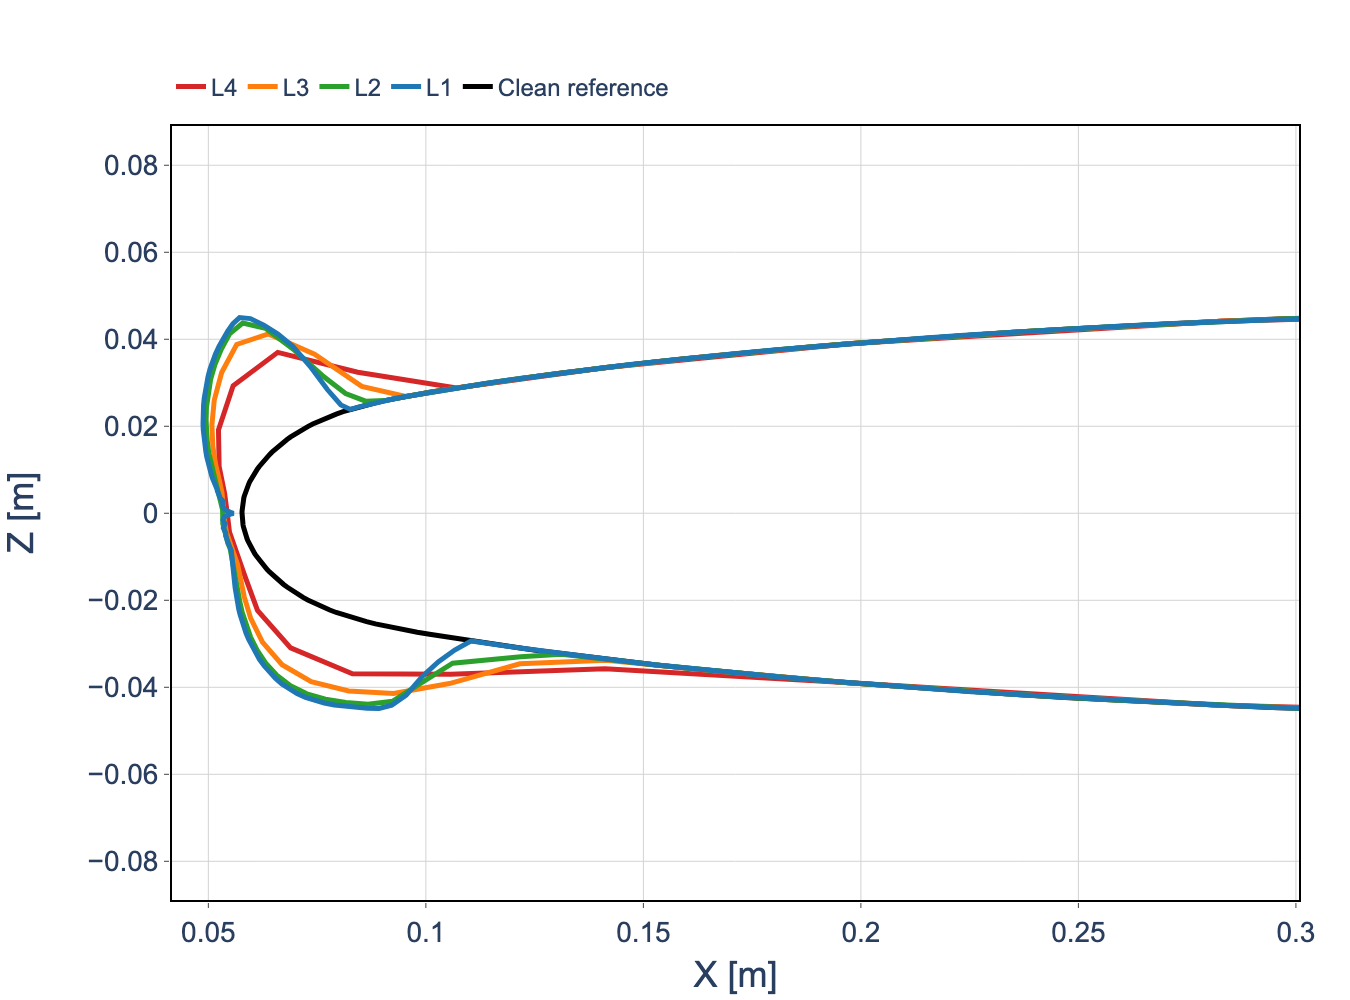
\includegraphics[
        width=\textwidth,
        trim={0cm 0cm 0cm 1.6cm},
        clip
    ]
    {FIGURES/ONERAM6/ICE_SHAPES/tc_oneram6_L1_single_layer_ice_shape_slice_0p1_bins07_roughness_1mm.png}
\end{column}

% ------------------------------------------------------------
% y = 0.75 m
% ------------------------------------------------------------
\begin{column}{0.333\textwidth}
    \centering
    \textbf{$y=0.75$ m}

    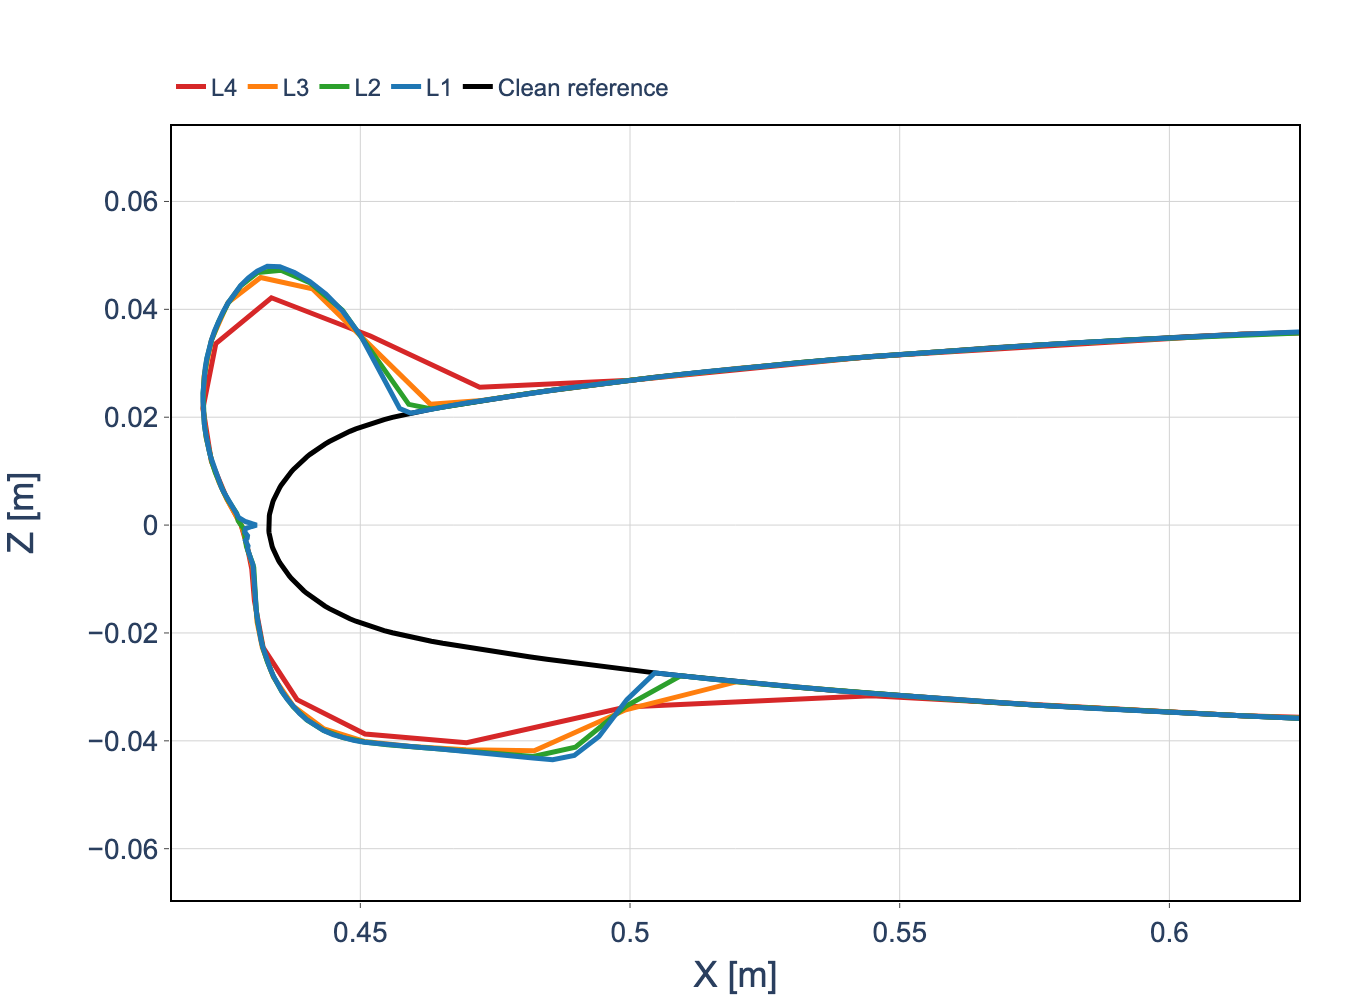
\includegraphics[
        width=\textwidth,
        trim={0cm 0cm 0cm 1.6cm},
        clip
    ]
    {FIGURES/ONERAM6/ICE_SHAPES/tc_oneram6_L1_single_layer_ice_shape_slice_0p75_bins07_roughness_1mm.png}
\end{column}

% ------------------------------------------------------------
% y = 1.40 m
% ------------------------------------------------------------
\begin{column}{0.333\textwidth}
    \centering
    \textbf{$y=1.40$ m}

    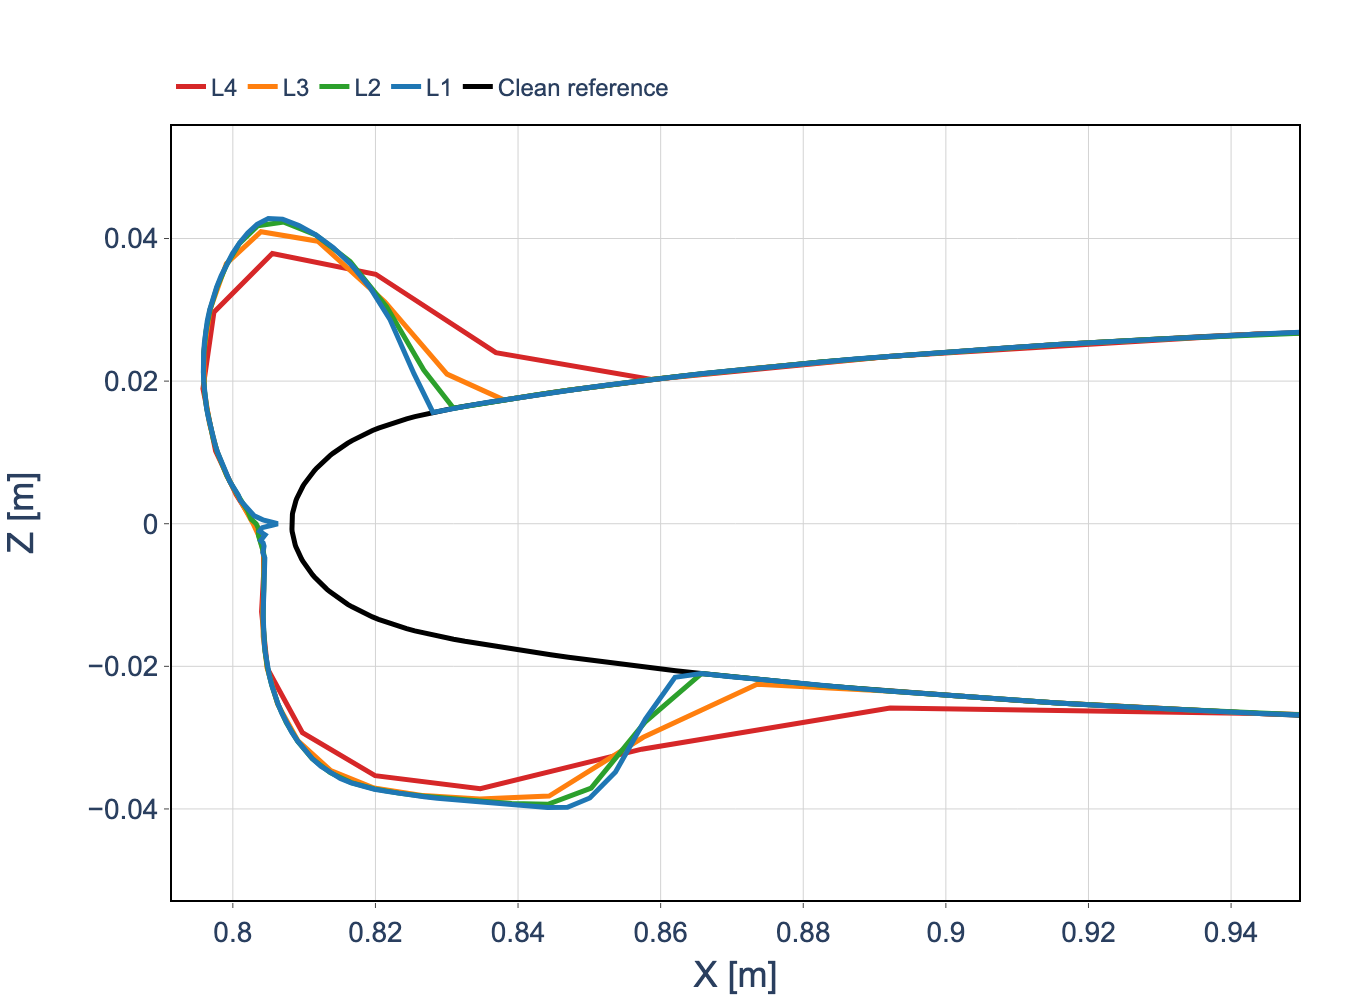
\includegraphics[
        width=\textwidth,
        trim={0cm 0cm 0cm 1.6cm},
        clip
    ]
    {FIGURES/ONERAM6/ICE_SHAPES/tc_oneram6_L1_single_layer_ice_shape_slice_1p4_bins07_roughness_1mm.png}
\end{column}

\end{columns}

\vspace{-0.10cm}

\begin{block}{\scriptsize Single-Layer Ice Shapes Assessment}
\begin{itemize}
    \item The single-layer ice shapes show limited sensitivity to spatial grid refinement, with L1--L3 providing similar predictions and the largest deviations observed on L4.
    \item The larger apparent impingement extent on L4 results from its coarser surface discretization rather than a physical shift in the impingement limits.
    \item The predicted horn geometry varies substantially along the span, with changes in both horn size and orientation between the three spanwise stations.
\end{itemize}
\end{block}

\end{frame}

% ============================================================
% ONERA M6 -- 3D Multilayer Ice Shape
% ============================================================

\begin{frame}{\small ONERA M6 -- Three-Dimensional Multilayer Ice Shape}
\scriptsize

\vspace{-0.20cm}

\centering
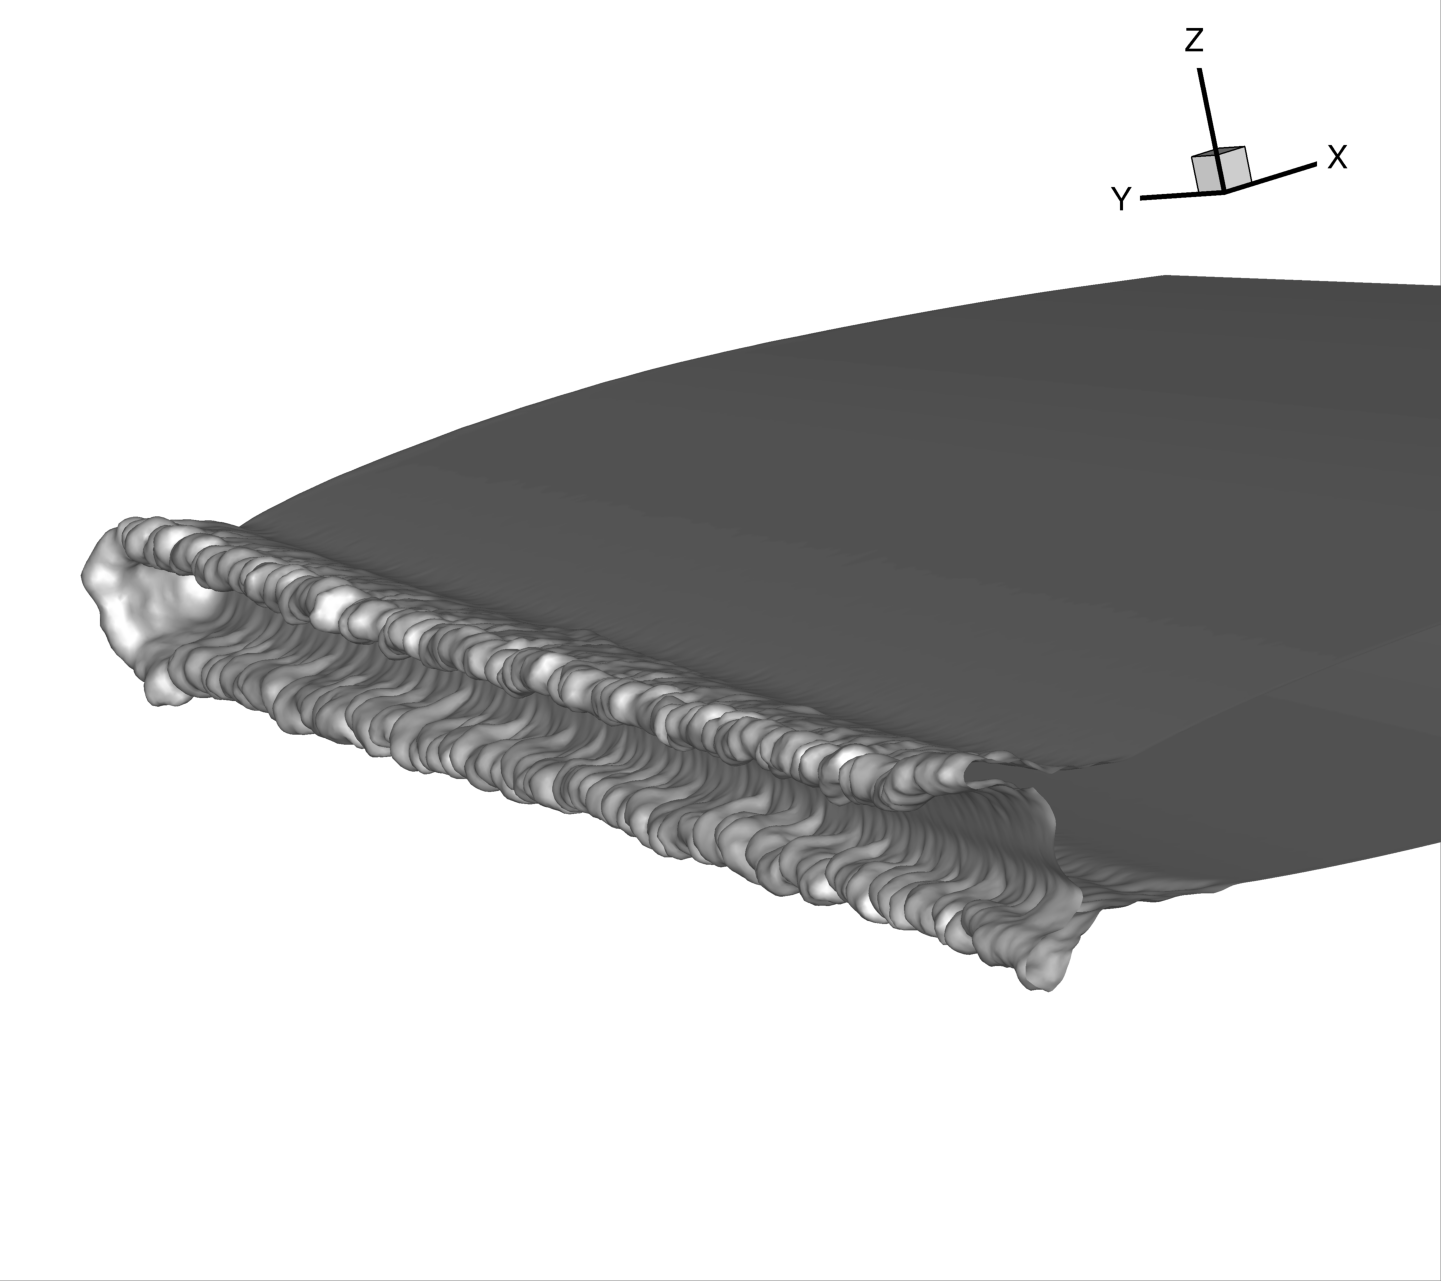
\includegraphics[
    width=0.5\textwidth,
    trim={0cm 5cm 0cm 0cm},
    clip
]
{FIGURES/ONERAM6/ICE_VIEWS/ONERAM6.png}

\vspace{-0.10cm}

\begin{block}{\scriptsize Multilayer Accretion}
The level-set approach captures the three-dimensional evolution of the ice geometry and the spanwise development of the horn structures.
\end{block}

\end{frame}


% ============================================================
% ONERA M6 -- Multilayer Ice Shapes
% ============================================================

\begin{frame}{\small ONERA M6 -- Multilayer Ice-Shape Comparison}
\scriptsize

\vspace{-0.15cm}

\begin{columns}[T,onlytextwidth]

% ------------------------------------------------------------
% y = 0.10 m
% ------------------------------------------------------------
\begin{column}{0.33\textwidth}
    \centering
    \textbf{$y=0.10$ m}

    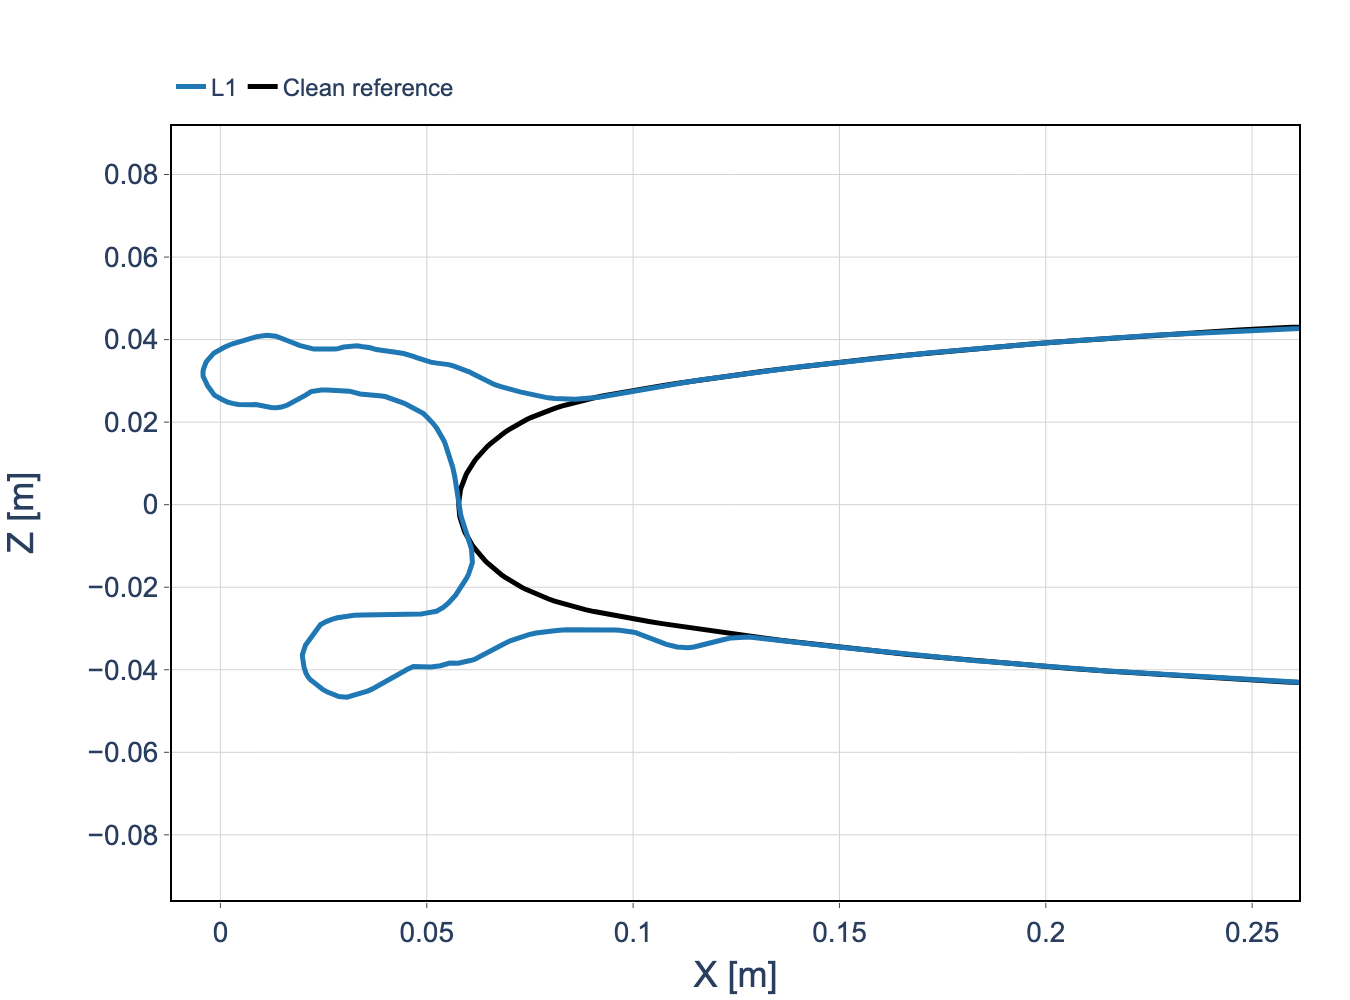
\includegraphics[
        width=\textwidth,
        trim={0cm 0cm 0cm 1.8cm},
        clip
    ]
    {FIGURES/ONERAM6/ICE_SHAPES/tc_oneram6_L1_multilayer_ice_shape_slice_0p1_bins07_roughness_1mm.png}
\end{column}

% ------------------------------------------------------------
% y = 0.75 m
% ------------------------------------------------------------
\begin{column}{0.33\textwidth}
    \centering
    \textbf{$y=0.75$ m}

    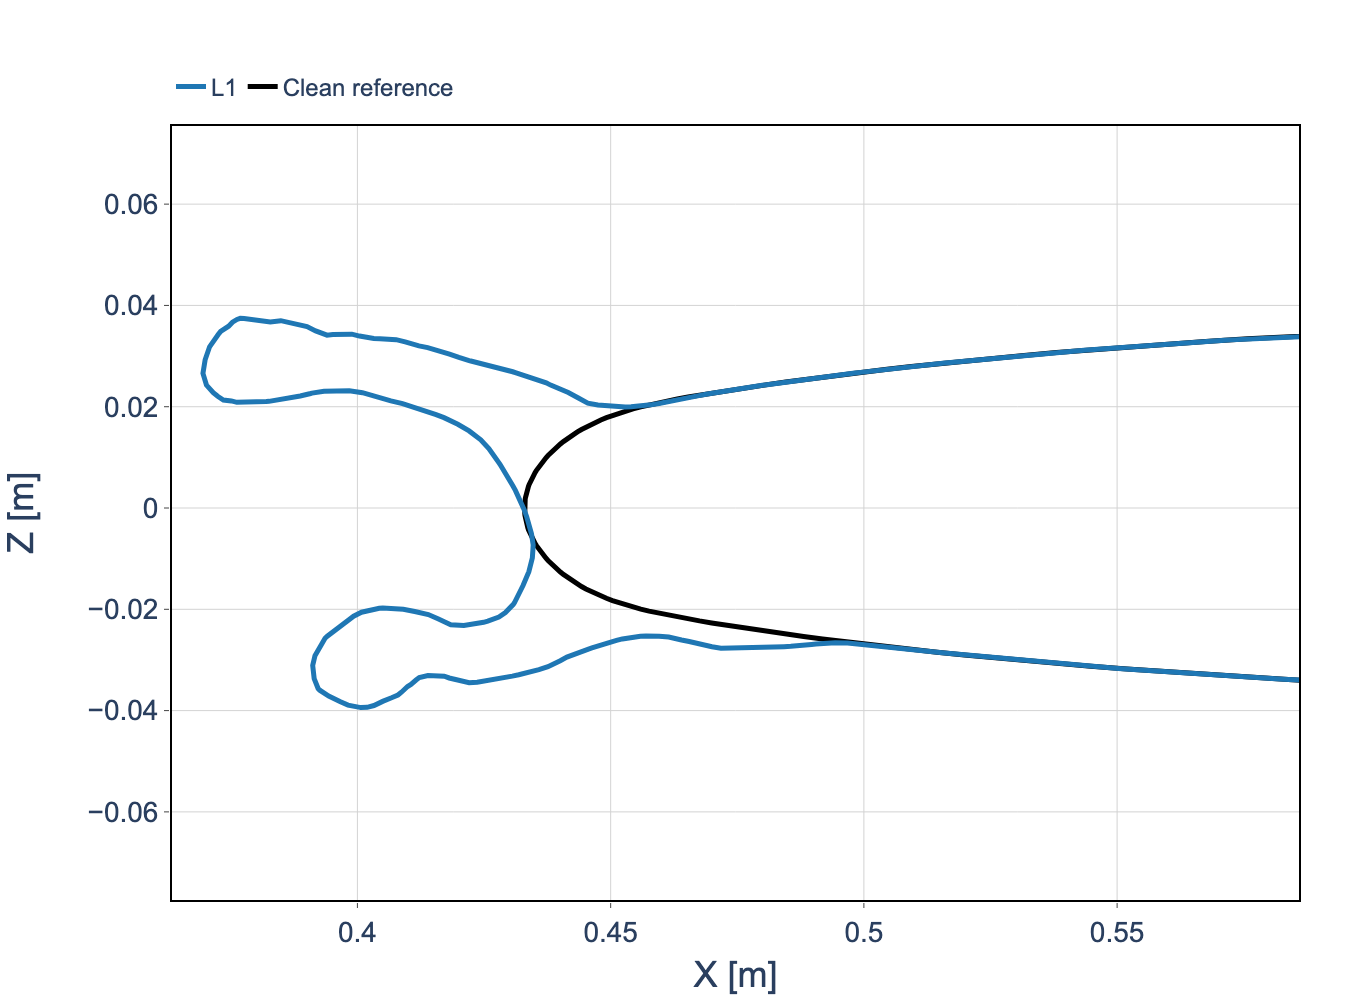
\includegraphics[
        width=\textwidth,
        trim={0cm 0cm 0cm 1.8cm},
        clip
    ]
    {FIGURES/ONERAM6/ICE_SHAPES/tc_oneram6_L1_multilayer_ice_shape_slice_0p75_bins07_roughness_1mm.png}
\end{column}

% ------------------------------------------------------------
% y = 1.40 m
% ------------------------------------------------------------
\begin{column}{0.33\textwidth}
    \centering
    \textbf{$y=1.40$ m}

    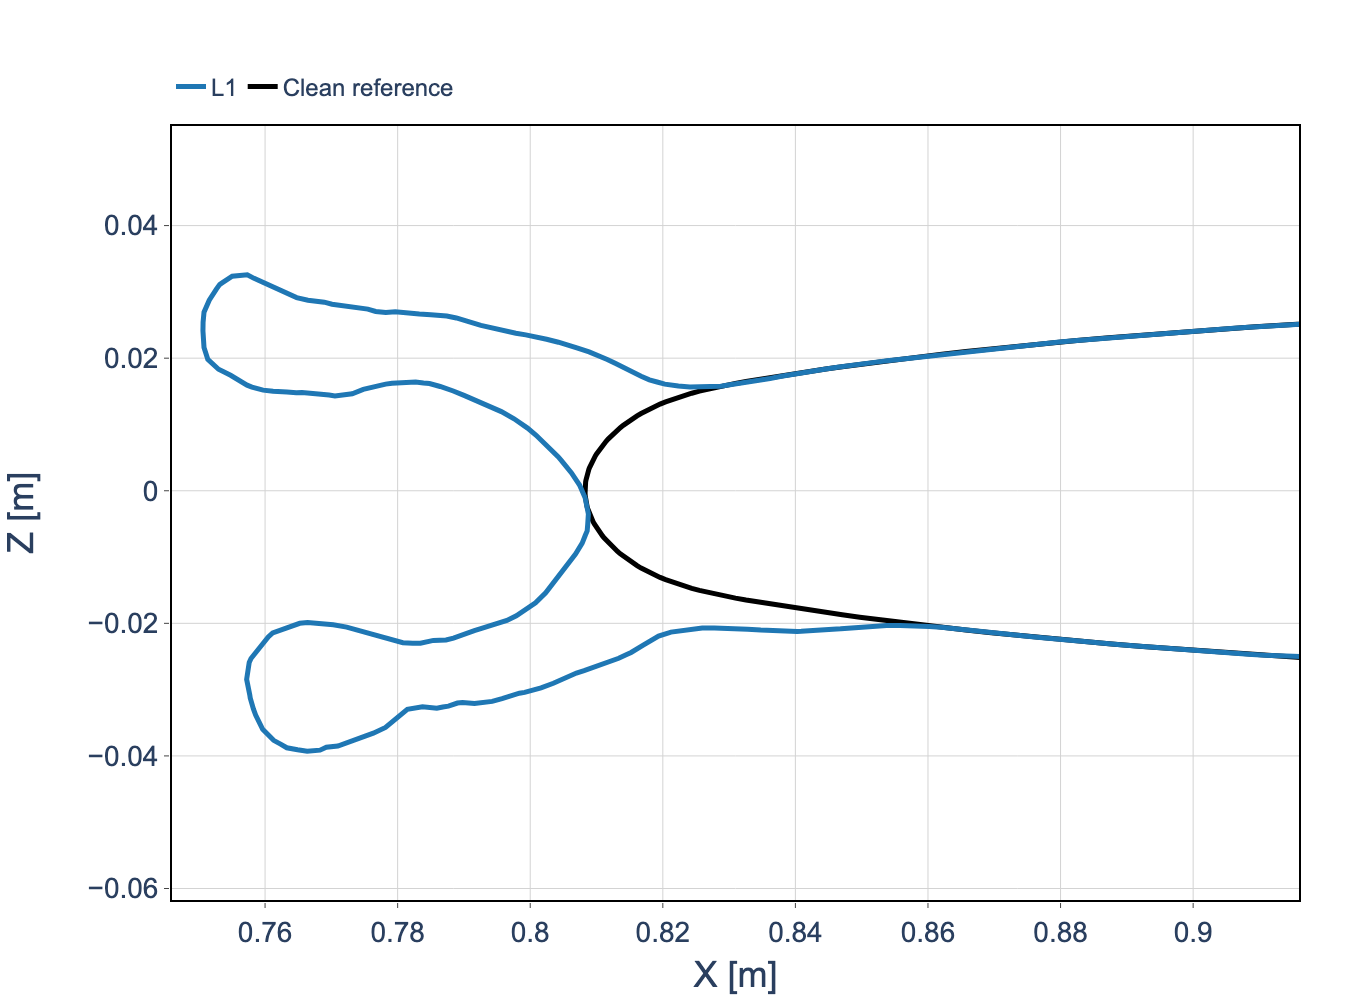
\includegraphics[
        width=\textwidth,
        trim={0cm 0cm 0cm 1.8cm},
        clip
    ]
    {FIGURES/ONERAM6/ICE_SHAPES/tc_oneram6_L1_multilayer_ice_shape_slice_1p4_bins07_roughness_1mm.png}
\end{column}

\end{columns}

\vspace{-0.10cm}

\begin{block}{\scriptsize Multilayer Ice Shapes Assessment}
\begin{itemize}
    \item CHAMPS predicts a consistent multilayer ice morphology across the three spanwise locations.
    \item The horn size and extent vary along the span, reflecting the three-dimensional development of the accretion.
\end{itemize}
\end{block}

\end{frame}
\section[Conclusion]{\textbf{Conclusion}}

% % ============================================================
% % COMPUTATIONAL COST
% % ============================================================

% \begin{frame}{\small Computational Cost and Numerical Setup}
% \scriptsize

% \vspace{-0.15cm}

% \begin{columns}[T,onlytextwidth]

% % ============================================================
% % LEFT
% % ============================================================
% \begin{column}{0.61\textwidth}

% % ------------------------------------------------------------
% % COMPUTATIONAL COST
% % ------------------------------------------------------------
% \begin{block}{\scriptsize Computational Cost}
% \centering

% \renewcommand{\arraystretch}{1.25}
% \setlength{\tabcolsep}{3.5pt}

% \begin{tabular}{lccc}
% \toprule
% \textbf{Computation}
% & \textbf{Mesh Size}
% & \textbf{Wall Time}
% & \textbf{Hardware} \\
% \midrule

% NACA0012 -- Flow
% & $\sim45$M
% & 58 min
% & Trillium \\

% NACA0012 -- Droplets (7 bins)
% & $\sim45$M
% & 90 min
% & Trillium \\

% ONERA M6 -- Flow
% & $\sim25$M
% & 70 min
% & Trillium \\

% ONERA M6 -- Droplets (7 bins)
% & $\sim25$M
% & 53 min
% & Trillium \\

% \midrule

% Level Set
% & $\sim10$M
% & $\sim18$ min
% & Xeon w7-2595X (26 cores) \\

% \bottomrule
% \end{tabular}

% \end{block}

% \vspace{0.08cm}

% % ------------------------------------------------------------
% % REMARKS
% % ------------------------------------------------------------
% \begin{alertblock}{\scriptsize Remarks}
% \begin{itemize}
%     \item NACA0012 surface mesh is extracted from the L1 grid and
%     diagonalized, substantially increasing the number of surface elements.

%     \item ONERA M6 surface mesh is generated directly from CAD; flow
%     convergence required a small initial CFL followed by progressive ramping.

%     \item Significant room remains for optimization of the numerical setup
%     and meshing strategy (surface meshing, CFL, etc.).

%     \item A leading-edge element size of approximately $1$--$2\,\mathrm{mm}$
%     provides the best results for capturing complex ice features with the
%     level-set approach.
% \end{itemize}
% \end{alertblock}

% \end{column}

% \hfill

% % ============================================================
% % RIGHT -- SURFACE MESH
% % ============================================================
% \begin{column}{0.36\textwidth}

%     \centering

%     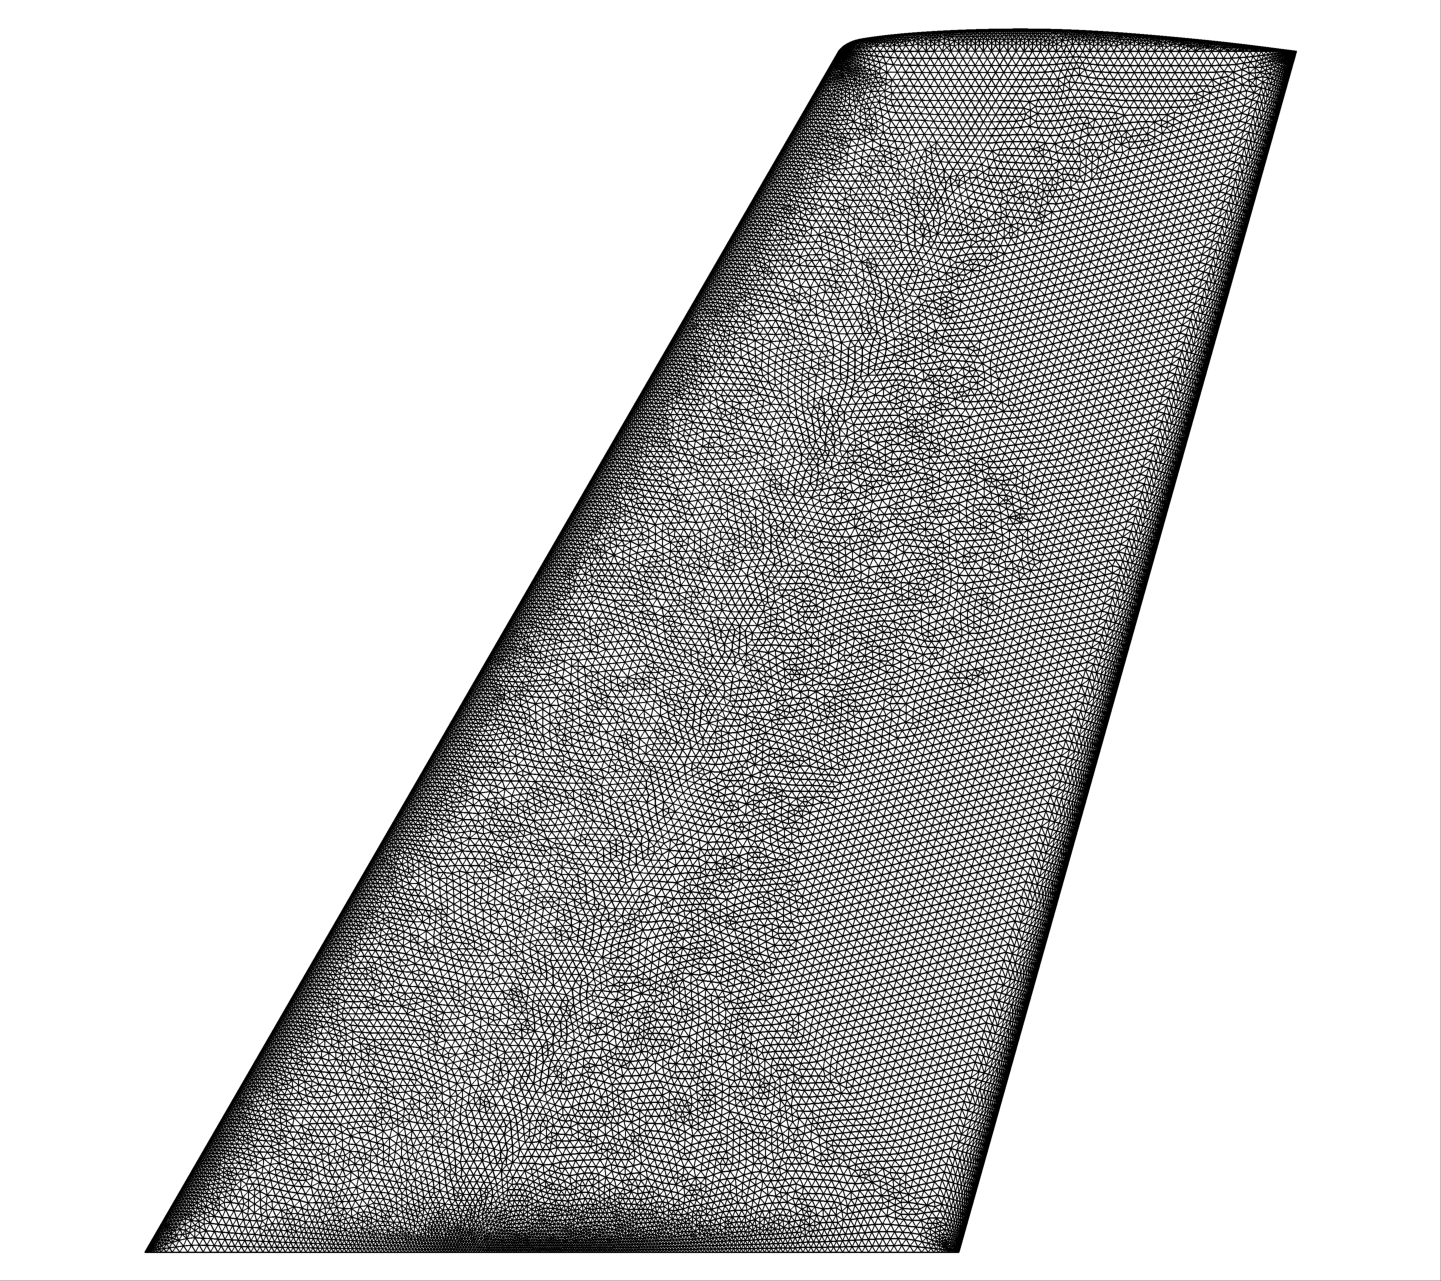
\includegraphics[
%         width=\textwidth,
%         height=0.76\textheight,
%         keepaspectratio
%     ]{FIGURES/ONERAM6/ICE_VIEWS/ONERA_M6_SURFACE_MESH.png}

%     \vspace{-0.05cm}

%     \textbf{ONERA M6 Surface Mesh}

%     \vspace{0.03cm}

%     {\scriptsize CAD-based triangular surface mesh}

% \end{column}

% \end{columns}

% \end{frame}

% ============================================================
% CONCLUSIONS
% ============================================================

\begin{frame}{\small Conclusions}
\scriptsize

% ------------------------------------------------------------
% GENERAL
% ------------------------------------------------------------
\begin{block}{\scriptsize General Findings}
\begin{itemize}
    \item Results are generally consistent across the grid hierarchy and well positioned within the IPW3 code-to-code envelope.
    \item Eulerian and Lagrangian droplet formulations show good agreement in collection efficiency and collected water mass.
\end{itemize}
\end{block}

\vspace{0.12cm}

% ------------------------------------------------------------
% NACA0012
% ------------------------------------------------------------
\begin{block}{\scriptsize NACA0012}
\begin{itemize}
    \item Single-layer ice shapes capture the experimental horn orientation well.
    \item Multilayer predictions show larger deviations in horn orientation, while capturing complex three-dimensional ice morphology.
\end{itemize}
\end{block}

\vspace{0.12cm}

% ------------------------------------------------------------
% ONERA M6
% ------------------------------------------------------------
\begin{block}{\scriptsize ONERA M6}
\begin{itemize}
    \item Single-layer ice shapes show limited grid sensitivity, with the largest deviations observed on L4.
    \item Multilayer simulations capture pronounced three-dimensional horn development and spanwise variations in the ice morphology.
\end{itemize}
\end{block}

\vspace{0.12cm}

% ------------------------------------------------------------
% OVERALL
% ------------------------------------------------------------
\begin{alertblock}{\scriptsize Overall}
\begin{itemize}
    \item CHAMPS provides a consistent end-to-end icing framework, with the level-set approach enabling complex three-dimensional ice geometries in multilayer simulations.
    \item Future work will focus on improving the roughness and ice-density models.
\end{itemize}
\end{alertblock}

\end{frame}

% ============================================================
% Acknowledgments
% ============================================================

\begin{frame}{\small Acknowledgments}
\scriptsize

\begin{itemize}
    \item This work is supported in part by a Bombardier/NSERC/CRIAQ Industrial Chair.

    \item Computations were performed on the Trillium supercomputer at the SciNet HPC Consortium, with computational resources provided through the Digital Research Alliance of Canada.

    %\item SciNet is funded by Innovation, Science and Economic Development Canada; the Digital Research Alliance of Canada; the Ontario Research Fund: Research Excellence; and the University of Toronto.
\end{itemize}

\end{frame}
% ============================================================
% BACKUP SLIDES
% ============================================================

\begin{frame}[plain]
    \centering
    \vfill

    {\LARGE\bfseries BACKUP SLIDES}

    \vfill
\end{frame}

% ============================================================
% NACA0012 -- HTC
% ============================================================

\begin{frame}{\small NACA0012 -- Convective Heat-Transfer Coefficient}
\scriptsize

\vspace{-0.15cm}

\begin{columns}[T,onlytextwidth]

% ------------------------------------------------------------
% AE3932
% ------------------------------------------------------------
\begin{column}{0.5\textwidth}
    \centering
    \textbf{AE3932}

    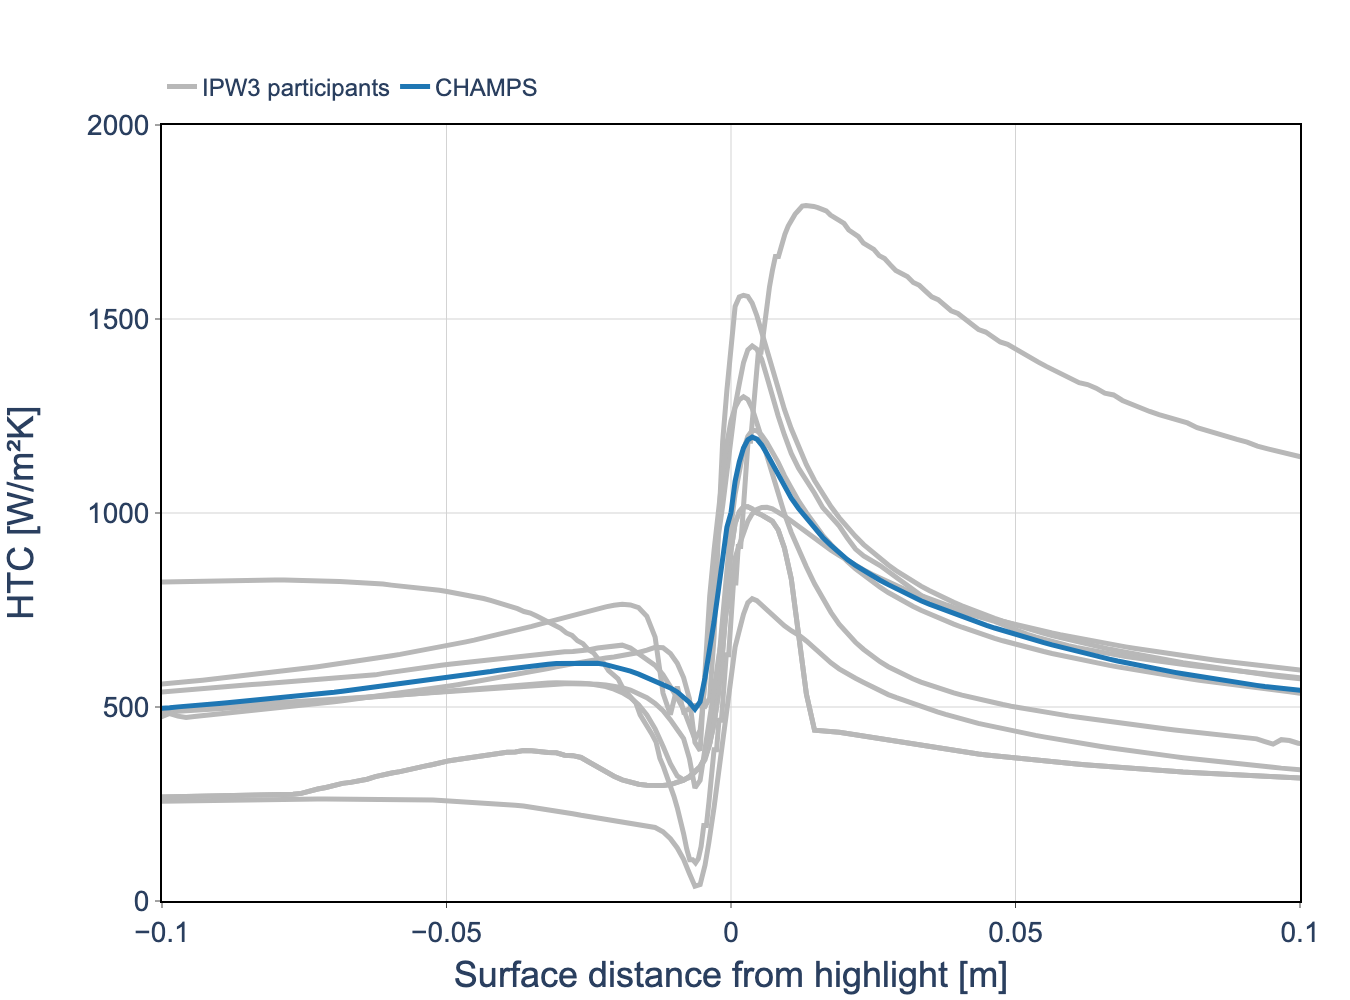
\includegraphics[
        width=\textwidth,
        trim={0cm 0cm 1cm 2.6cm},
        clip
    ]
    {FIGURES/NACA0012/HTC/tc_naca0012_ae3932_L1_htc_vs_s_slice_0p9144_all_roughness.png}
\end{column}

\hspace{-0.04\textwidth}

% ------------------------------------------------------------
% AE3933
% ------------------------------------------------------------
\begin{column}{0.5\textwidth}
    \centering
    \textbf{AE3933}
    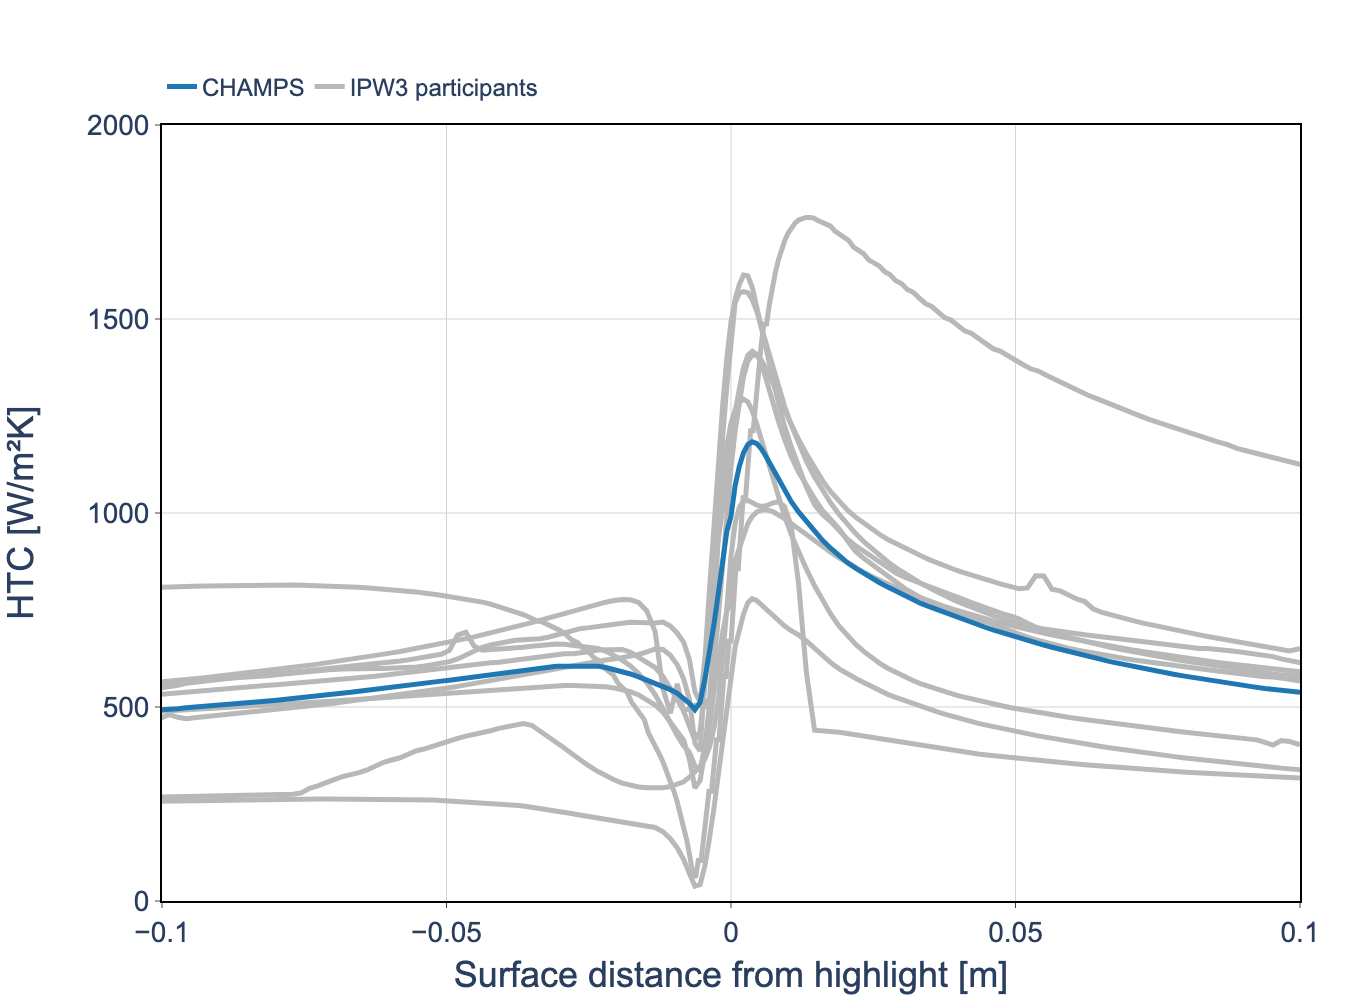
\includegraphics[
        width=\textwidth,
        trim={0cm 0cm 1cm 2.6cm},
        clip
    ]
    {FIGURES/NACA0012/HTC/tc_naca0012_ae3933_L1_htc_vs_s_slice_0p9144_all_roughness.png}
\end{column}

\end{columns}

\vspace{-0.15cm}

\end{frame}

% ============================================================
% BACKUP -- NACA0012 Freezing Fraction
% ============================================================

\begin{frame}{\small NACA0012 -- Freezing Fraction}
\scriptsize

\vspace{-0.15cm}

\begin{columns}[T,onlytextwidth]

% ------------------------------------------------------------
% AE3932
% ------------------------------------------------------------
\begin{column}{0.50\textwidth}
    \centering
    \textbf{AE3932}

    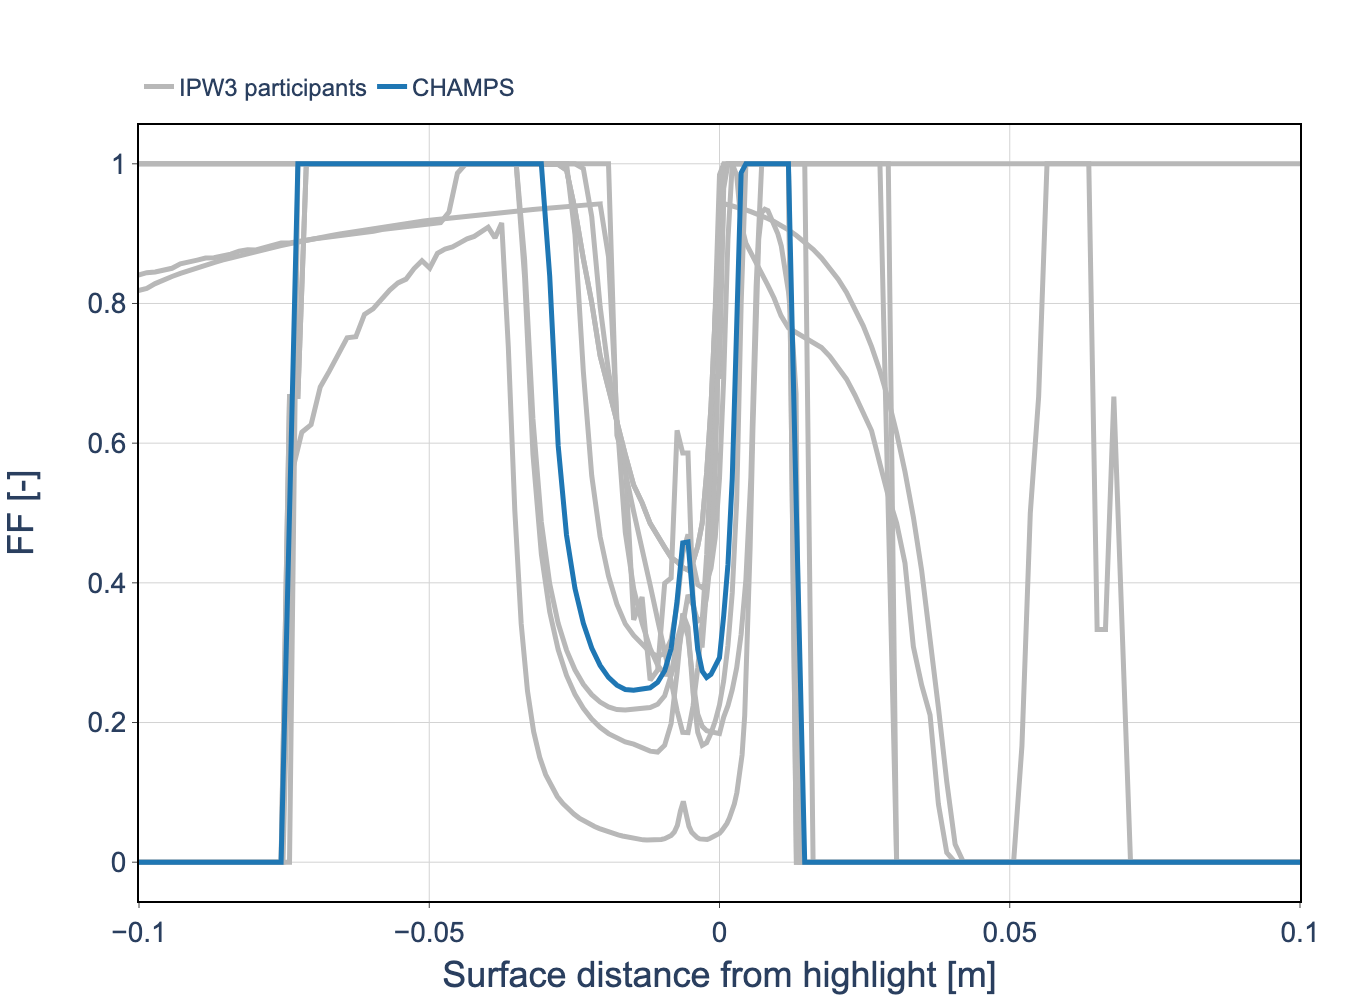
\includegraphics[
        width=\textwidth,
        trim={0cm 0cm 0cm 1.8cm},
        clip
    ]
    {FIGURES/NACA0012/SURF_TEMP_FF/tc_naca0012_ae3932_L1_freezing_fraction_vs_s_slice_0p9144_all_roughness.png}
\end{column}

% ------------------------------------------------------------
% AE3933
% ------------------------------------------------------------
\begin{column}{0.50\textwidth}
    \centering
    \textbf{AE3933}

    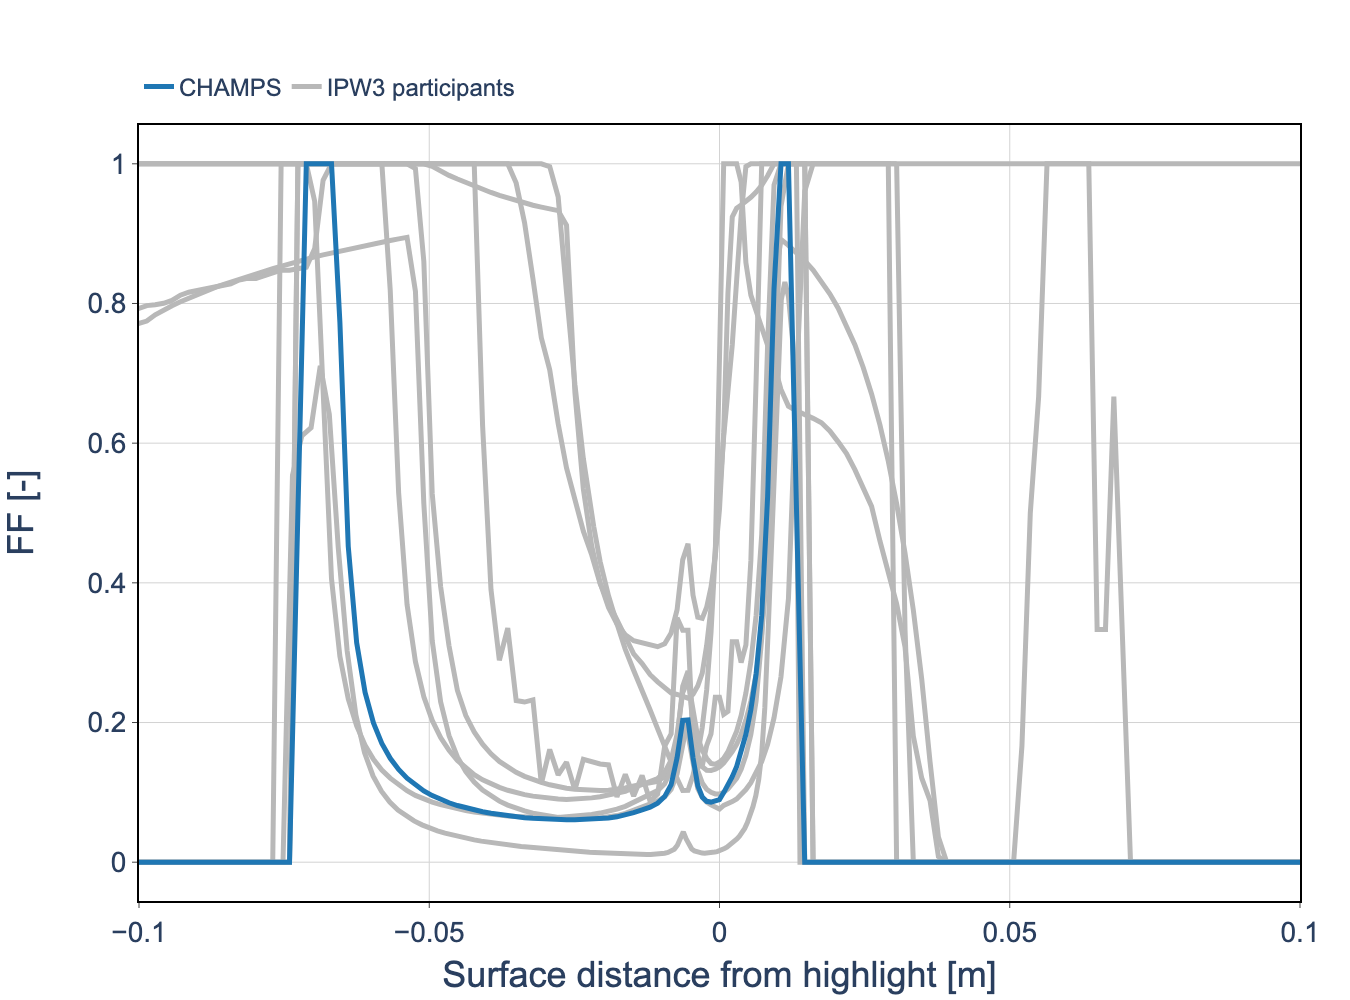
\includegraphics[
        width=\textwidth,
        trim={0cm 0cm 0cm 1.8cm},
        clip
    ]
    {FIGURES/NACA0012/SURF_TEMP_FF/tc_naca0012_ae3933_L1_freezing_fraction_vs_s_slice_0p9144_all_roughness.png}
\end{column}

\end{columns}

\end{frame}


% ============================================================
% BACKUP -- NACA0012 Surface Temperature
% ============================================================

\begin{frame}{\small NACA0012 -- Surface Temperature}
\scriptsize

\vspace{-0.15cm}

\begin{columns}[T,onlytextwidth]

% ------------------------------------------------------------
% AE3932
% ------------------------------------------------------------
\begin{column}{0.50\textwidth}
    \centering
    \textbf{AE3932}

    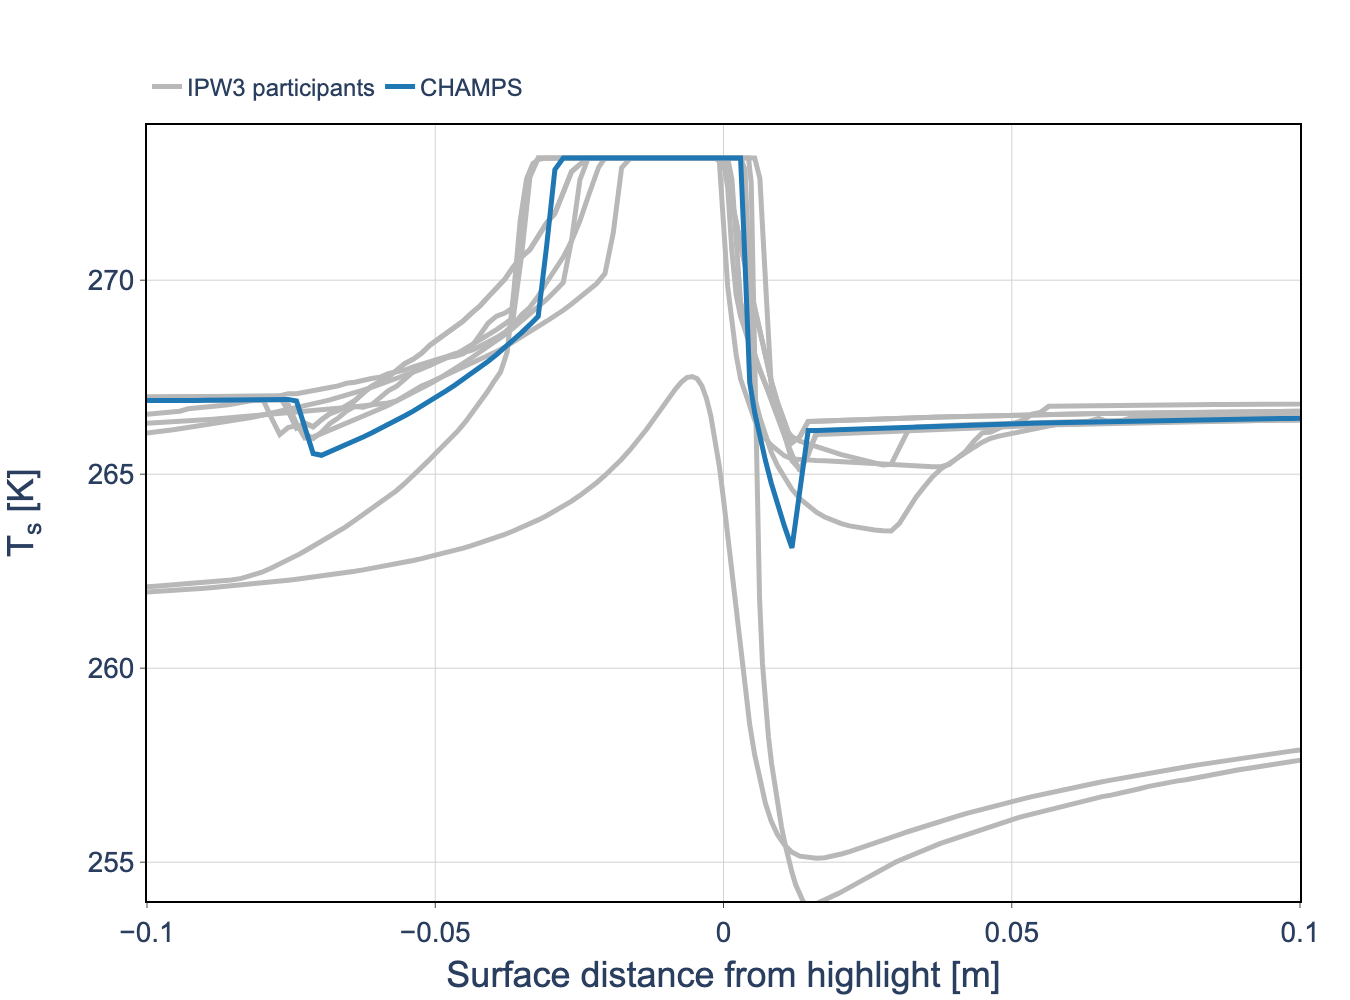
\includegraphics[
        width=\textwidth,
        trim={0cm 0cm 0cm 1.8cm},
        clip
    ]
    {FIGURES/NACA0012/SURF_TEMP_FF/tc_naca0012_ae3932_L1_surface_temperature_vs_s_slice_0p9144_all_roughness.png}
\end{column}

% ------------------------------------------------------------
% AE3933
% ------------------------------------------------------------
\begin{column}{0.50\textwidth}
    \centering
    \textbf{AE3933}

    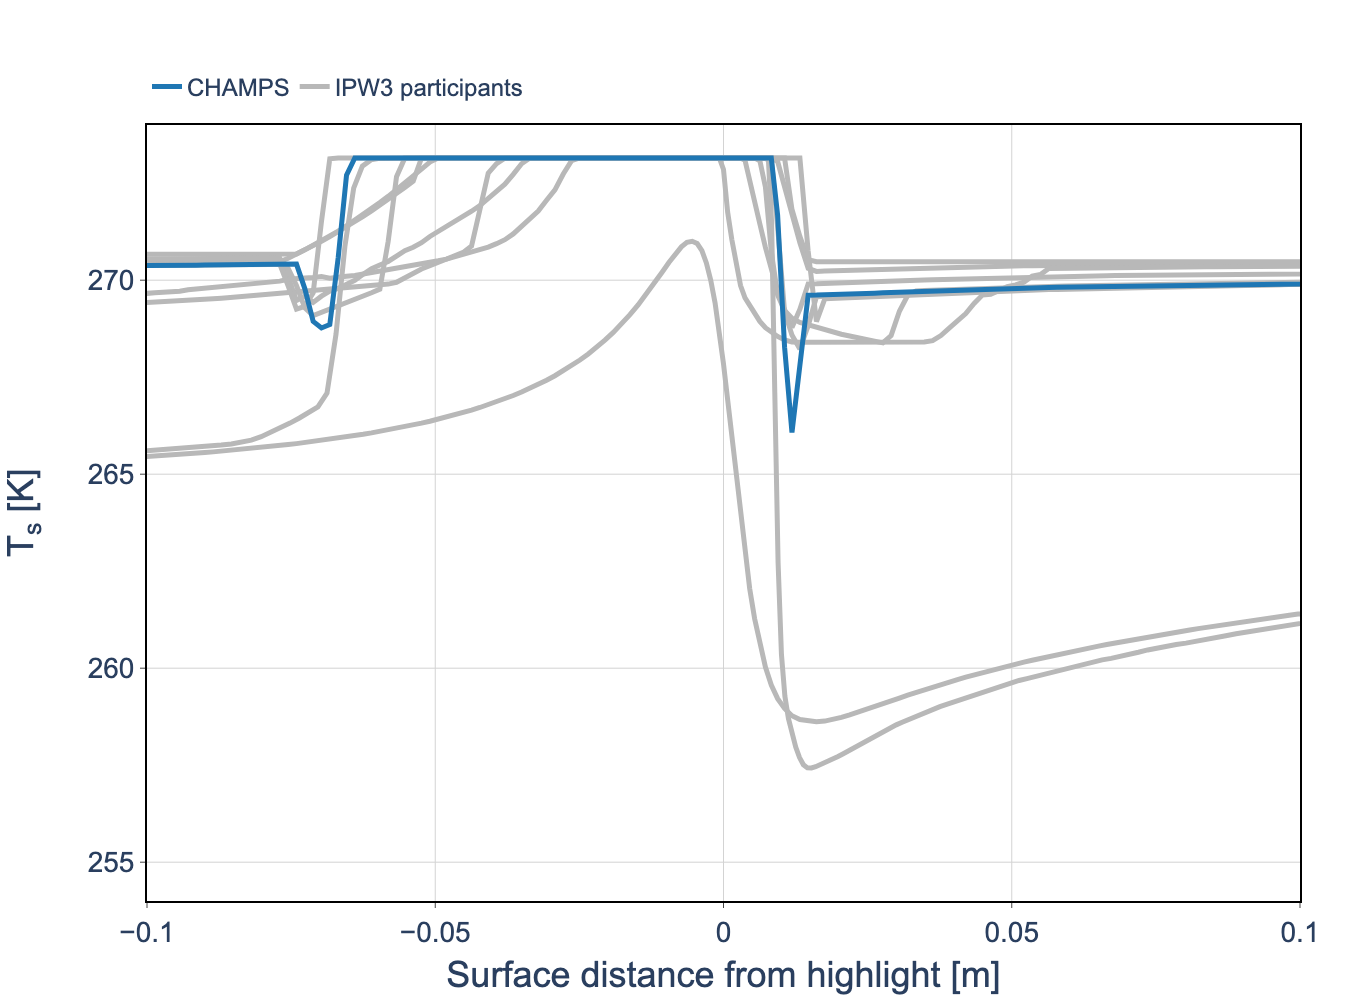
\includegraphics[
        width=\textwidth,
        trim={0cm 0cm 0cm 1.8cm},
        clip
    ]
    {FIGURES/NACA0012/SURF_TEMP_FF/tc_naca0012_ae3933_L1_surface_temperature_vs_s_slice_0p9144_all_roughness.png}
\end{column}

\end{columns}

\end{frame}


% ============================================================
% NACA0012 -- Upper-Horn Angle
% ============================================================

\begin{frame}{\small NACA0012 -- Upper-Horn Angle}
\scriptsize

\vspace{-0.15cm}

\begin{columns}[T,onlytextwidth]

% ------------------------------------------------------------
% AE3932
% ------------------------------------------------------------
\begin{column}{0.50\textwidth}
    \centering
    \textbf{AE3932}

    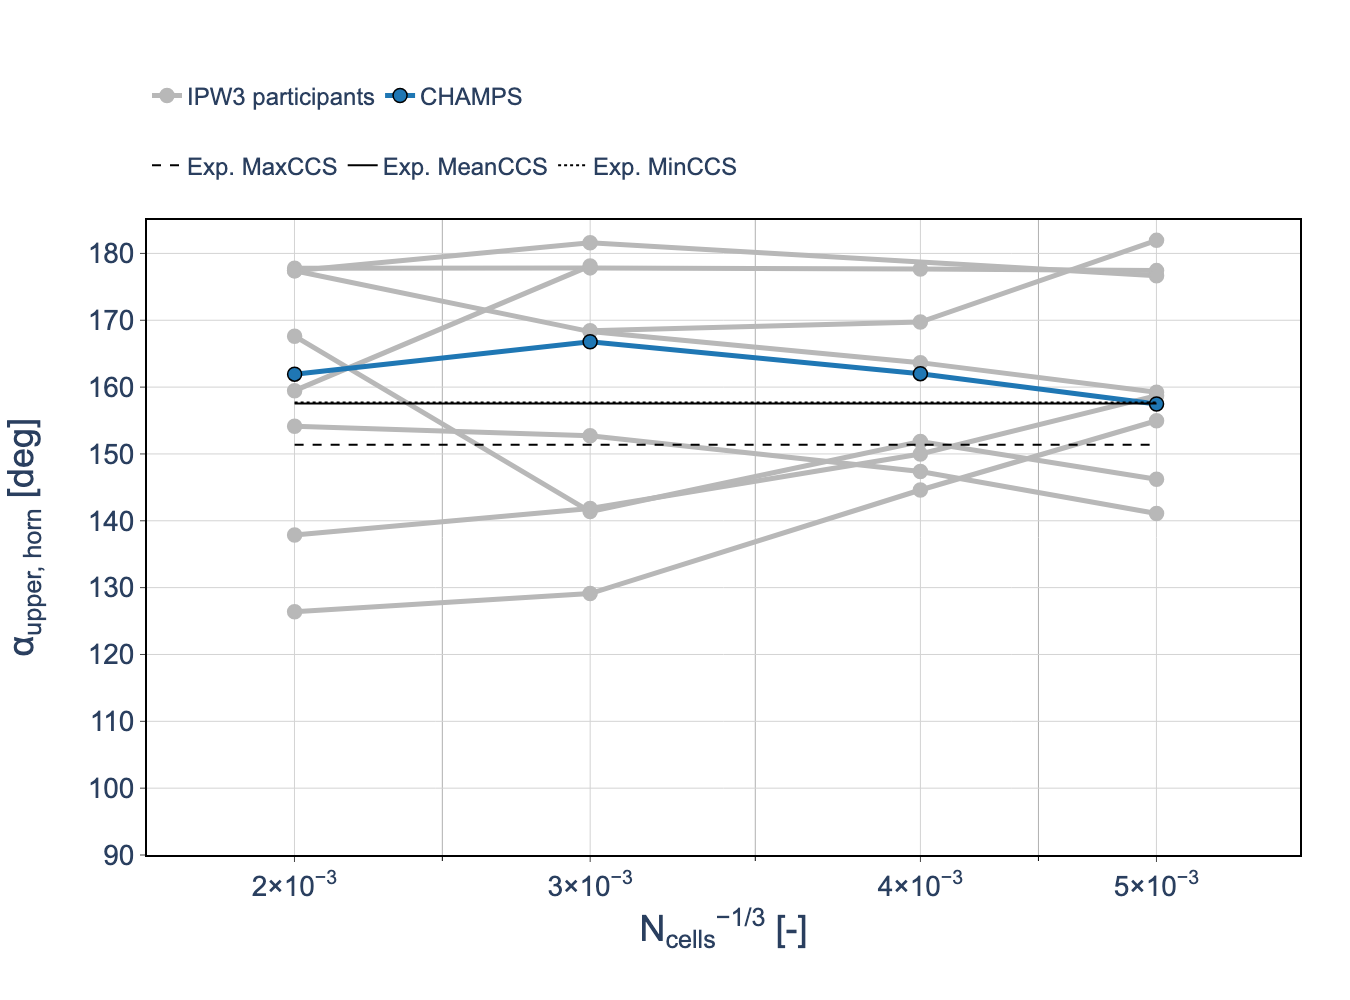
\includegraphics[
        width=\textwidth,
        trim={0cm 1cm 1cm 2.6cm},
        clip
    ]
    {FIGURES/NACA0012/ICE_ACCRETION/tc_naca0012_ae3932_upper_horn_angle_bins15.png}
\end{column}

% ------------------------------------------------------------
% AE3933
% ------------------------------------------------------------
\begin{column}{0.50\textwidth}
    \centering
    \textbf{AE3933}

    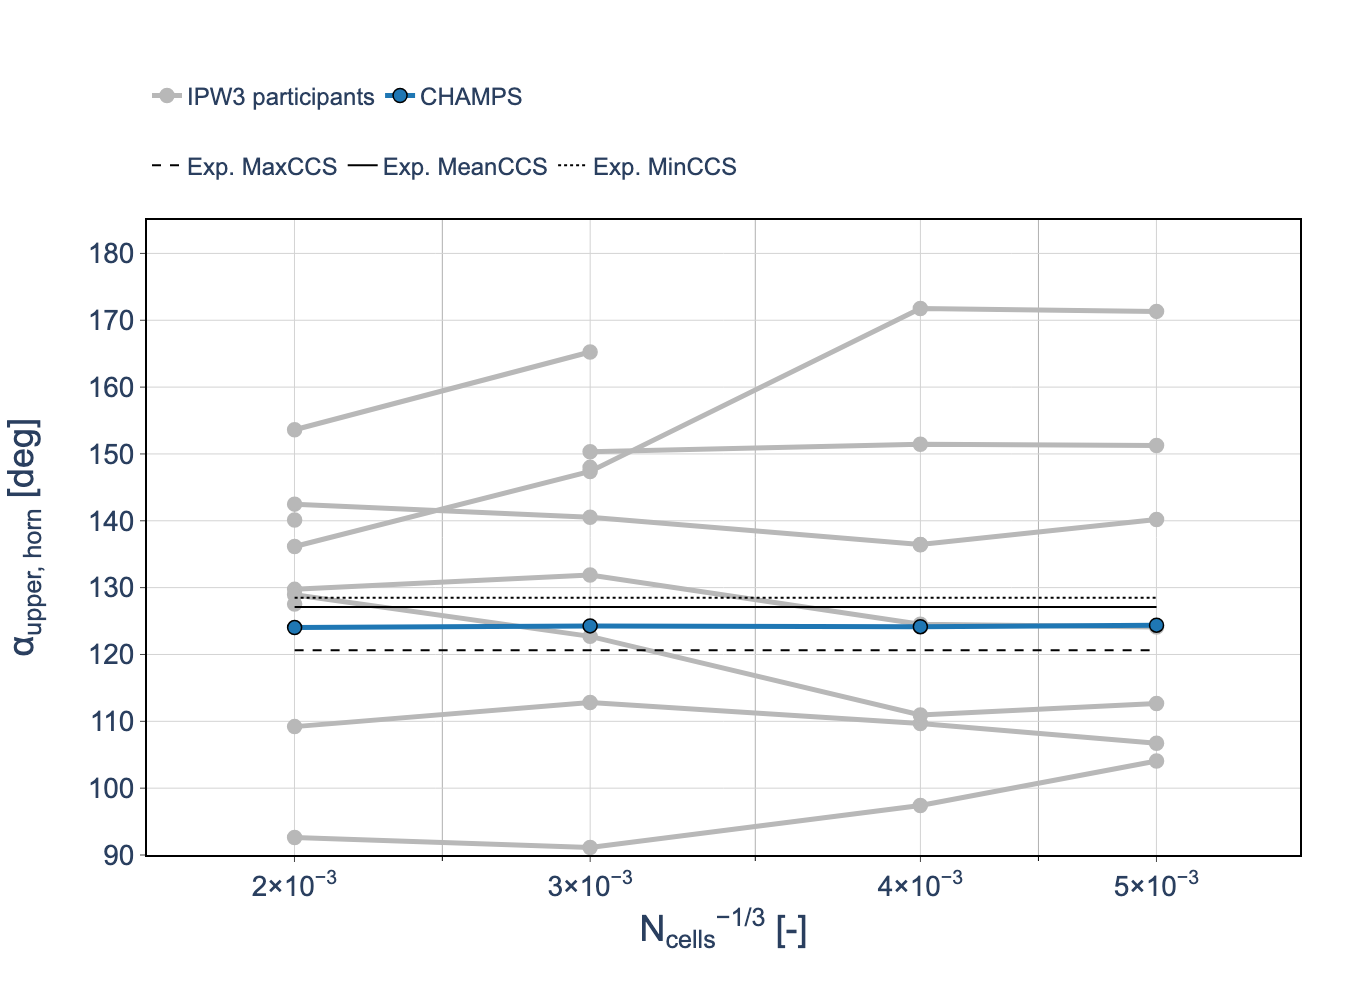
\includegraphics[
        width=\textwidth,
        trim={0cm 1cm 1cm 2.6cm},
        clip
    ]
    {FIGURES/NACA0012/ICE_ACCRETION/tc_naca0012_ae3933_upper_horn_angle_bins15.png}
\end{column}

\end{columns}

\vspace{-0.10cm}

\begin{block}{\scriptsize Assessment}
\begin{itemize}
    \item The predicted upper-horn angles agree well with experiment for both icing conditions.
    \item Droplet-bin refinement has negligible influence on the upper-horn angle (not shown due to limited variation).
    \item The substantial decrease in upper-horn angle from AE3932 to AE3933 is well captured.
\end{itemize}
\end{block}

\end{frame}

% ============================================================
% NACA0012 -- Multilayer Maximum Cross Sections
% ============================================================

\begin{frame}{\small NACA0012 -- Multilayer Maximum Cross Sections}
\scriptsize

\vspace{-0.15cm}

\begin{columns}[T,onlytextwidth]

% ------------------------------------------------------------
% AE3932
% ------------------------------------------------------------
\begin{column}{0.50\textwidth}
    \centering
    \textbf{AE3932}

    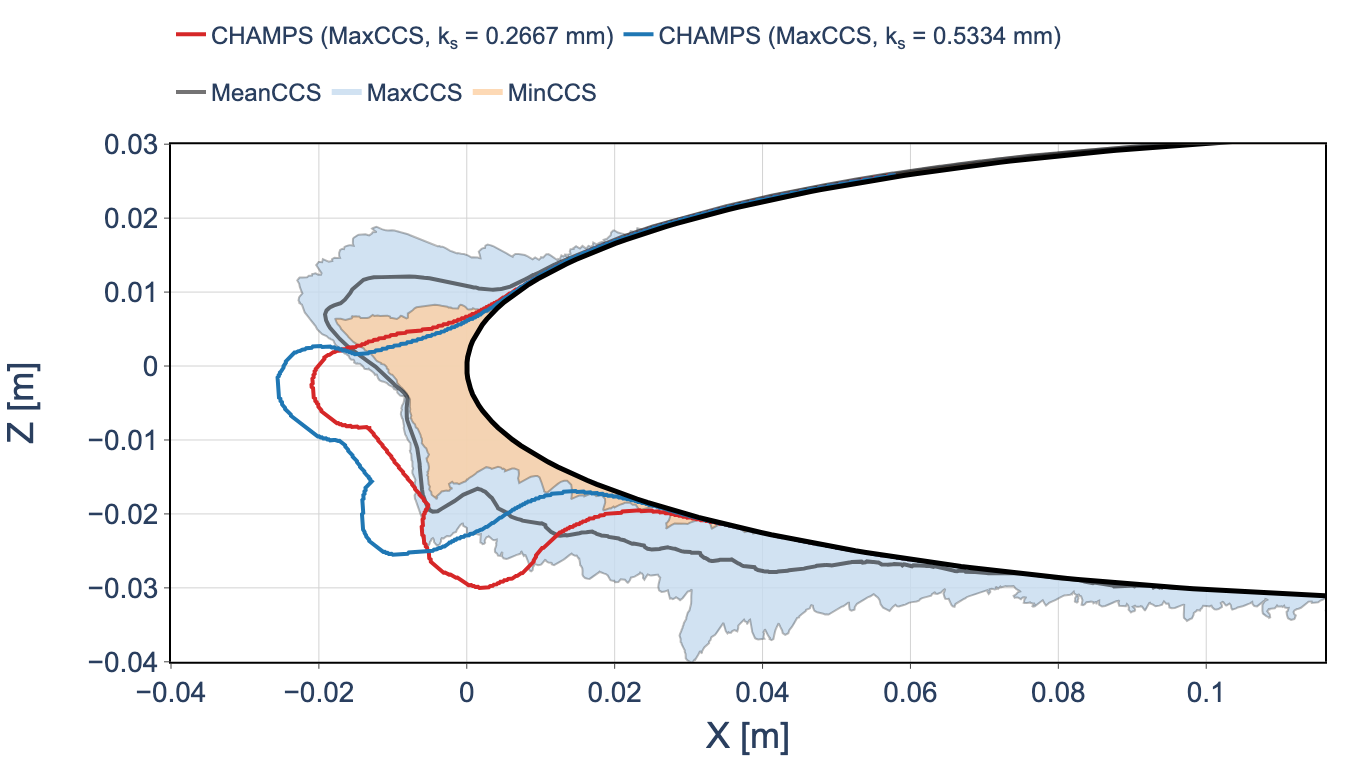
\includegraphics[
        width=\textwidth,
        trim={0cm 0cm 1cm 0.8cm},
        clip
    ]
    {FIGURES/NACA0012/ICE_SHAPES/tc_naca0012_ae3932_L1_multilayer_ice_shape_slice_0p9144_bins07_roughness_comparisons_MCCS.png}
\end{column}

% ------------------------------------------------------------
% AE3933
% ------------------------------------------------------------
\begin{column}{0.50\textwidth}
    \centering
    \textbf{AE3933}

    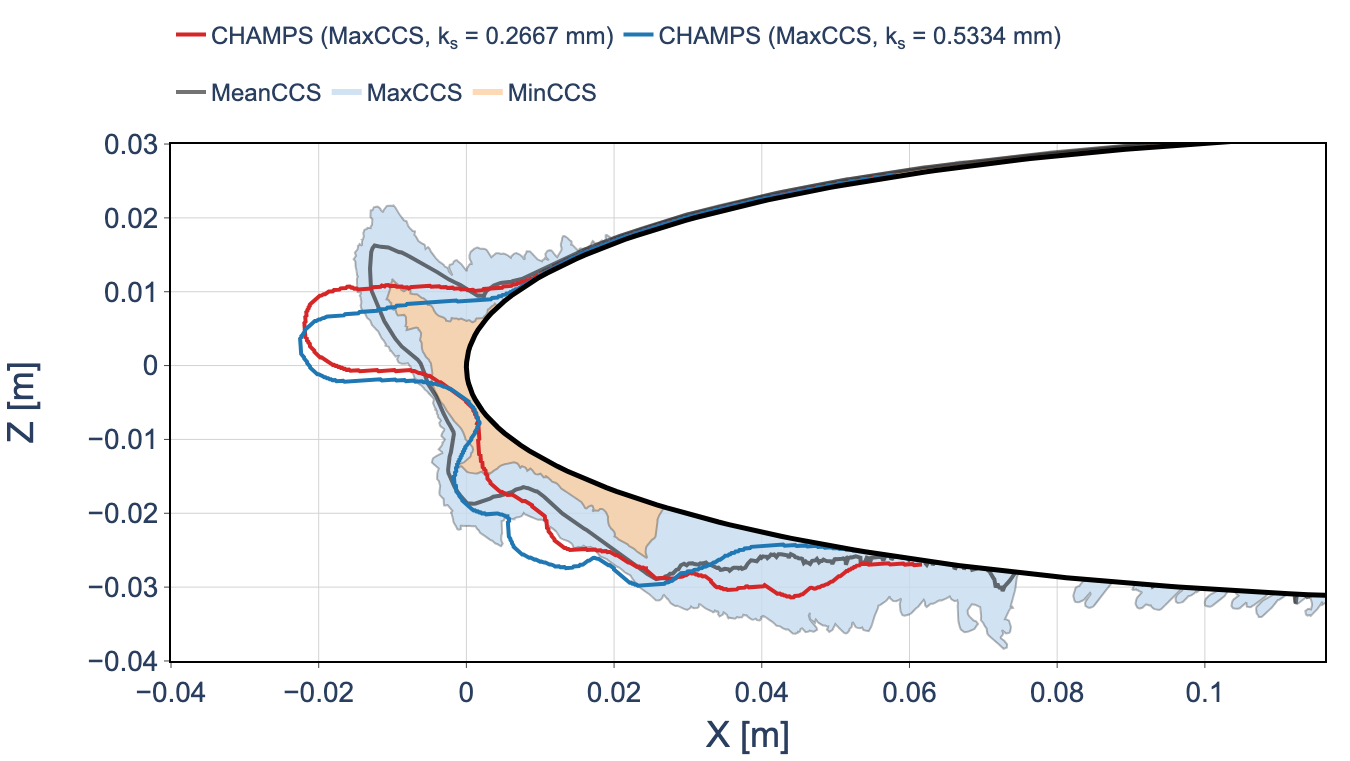
\includegraphics[
        width=\textwidth,
        trim={0cm 0cm 1cm 0.8cm},
        clip
    ]
    {FIGURES/NACA0012/ICE_SHAPES/tc_naca0012_ae3933_L1_multilayer_ice_shape_slice_0p9144_bins07_roughness_comparisons_MCCS.png}
\end{column}

\end{columns}

\vspace{-0.10cm}

\end{frame}

% ============================================================
% NACA0012 -- Effect of Surface-Normal Update
% ============================================================

\begin{frame}{\small NACA0012 -- Effect of Surface-Normal Update}
\scriptsize

\vspace{-0.15cm}

\begin{columns}[T,onlytextwidth]

% ------------------------------------------------------------
% AE3932
% ------------------------------------------------------------
\begin{column}{0.50\textwidth}
    \centering
    \textbf{AE3932}

    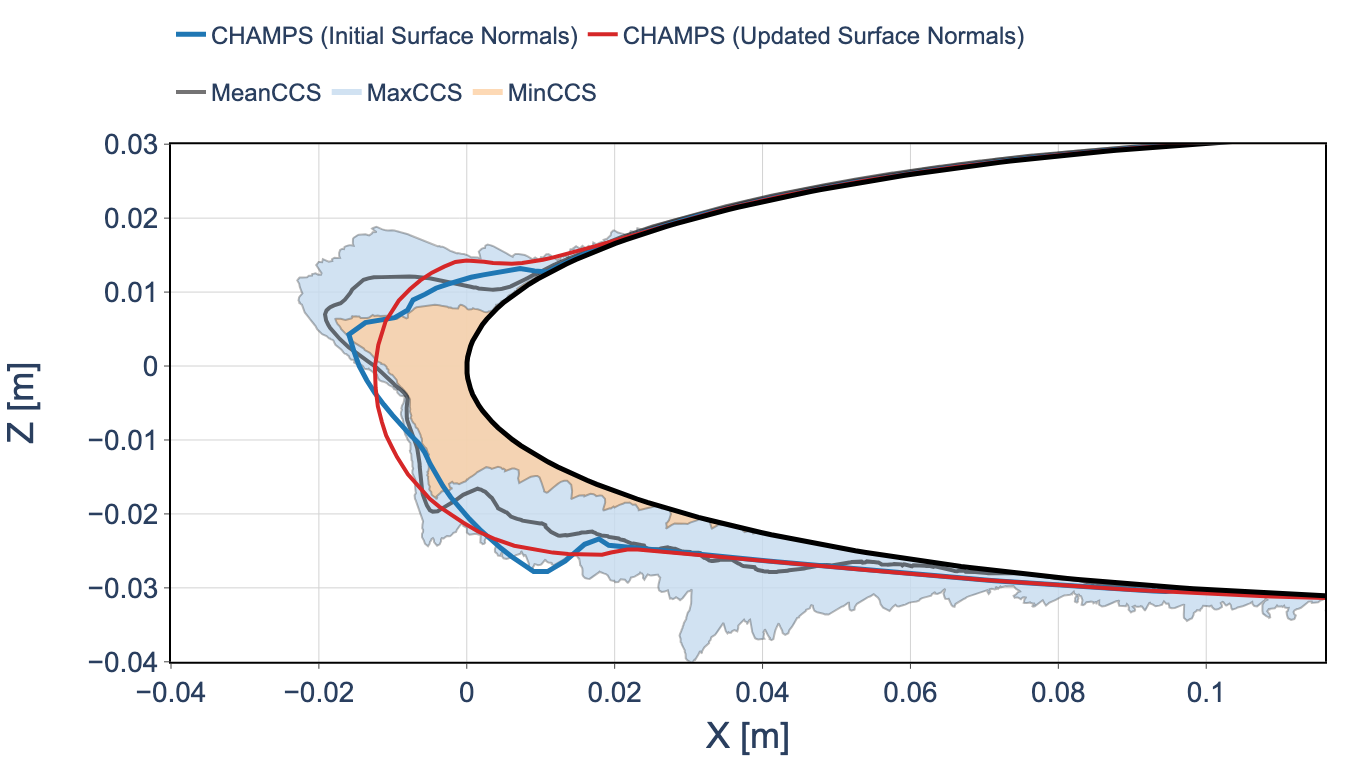
\includegraphics[
        width=\textwidth,
        trim={0cm 0cm 0cm 0.8cm},
        clip
    ]
    {FIGURES/NACA0012/ICE_SHAPES/tc_naca0012_ae3932_L1_single_layer_ice_shape_slice_0p9144_bins15_normals_comparison.png}
\end{column}

% ------------------------------------------------------------
% AE3933
% ------------------------------------------------------------
\begin{column}{0.50\textwidth}
    \centering
    \textbf{AE3933}

    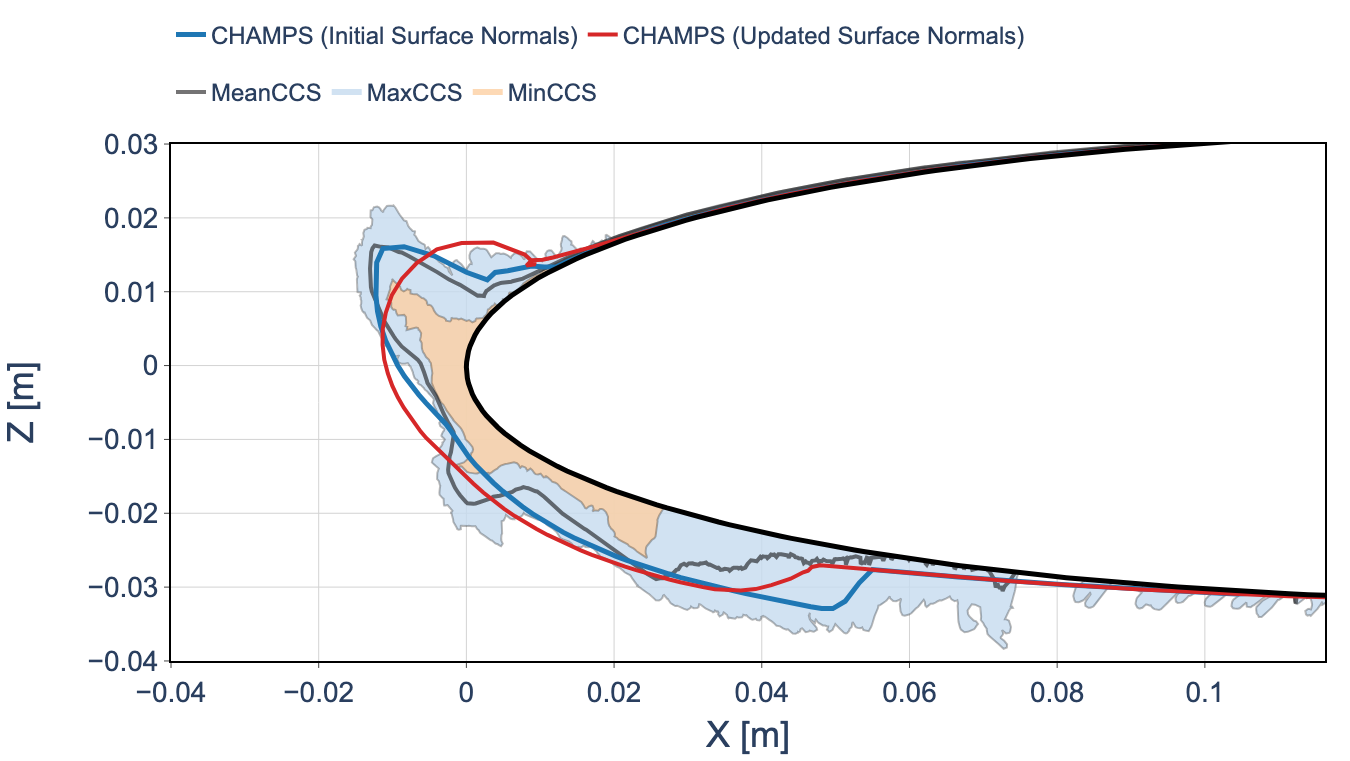
\includegraphics[
        width=\textwidth,
        trim={0cm 0cm 0cm 0.8cm},
        clip
    ]
    {FIGURES/NACA0012/ICE_SHAPES/tc_naca0012_ae3933_L1_single_layer_ice_shape_slice_0p9144_bins15_normals_comparison.png}
\end{column}

\end{columns}

\vspace{-0.10cm}

\begin{block}{\scriptsize Assessment}
\begin{itemize}
    \item Updating the surface normals while retaining the original surface accretion map produces a blunter horn and modifies its orientation.

    \item Retaining the initial normals provides better agreement with the experimental horn orientation for the present algebraic displacement.

    \item The updating of the surface accretion solution with the evolving normals was not considered in the present approach and will be investigated further.
\end{itemize}
\end{block}

\end{frame}



% ============================================================
% BACKUP -- ONERA M6 Convective Heat Transfer
% ============================================================

\begin{frame}{\small ONERA M6 -- Convective Heat-Transfer Coefficient}
\scriptsize

\vspace{-0.20cm}

\begin{columns}[T,onlytextwidth]

% ------------------------------------------------------------
% y = 0.10 m
% ------------------------------------------------------------
\begin{column}{0.33\textwidth}
    \centering
    \textbf{$y=0.10$ m}

    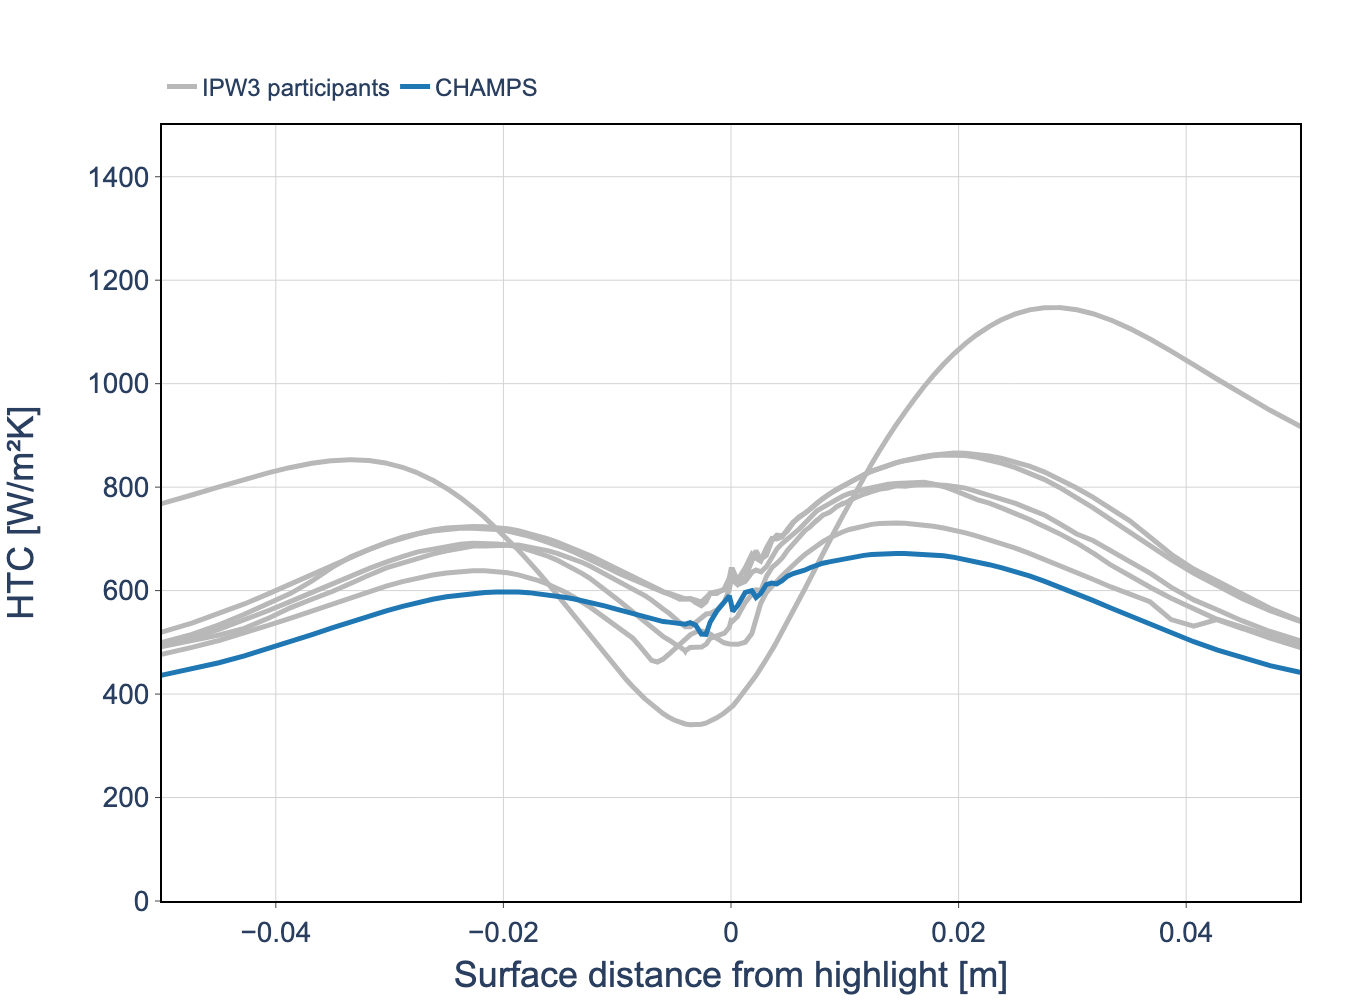
\includegraphics[
        width=\textwidth,
        trim={0cm 0cm 1cm 3.2cm},
        clip
    ]
    {FIGURES/ONERAM6/HTC/tc_oneram6_L1_htc_vs_s_slice_0p1_roughness_1mm.png}
\end{column}

% ------------------------------------------------------------
% y = 0.75 m
% ------------------------------------------------------------
\begin{column}{0.33\textwidth}
    \centering
    \textbf{$y=0.75$ m}

    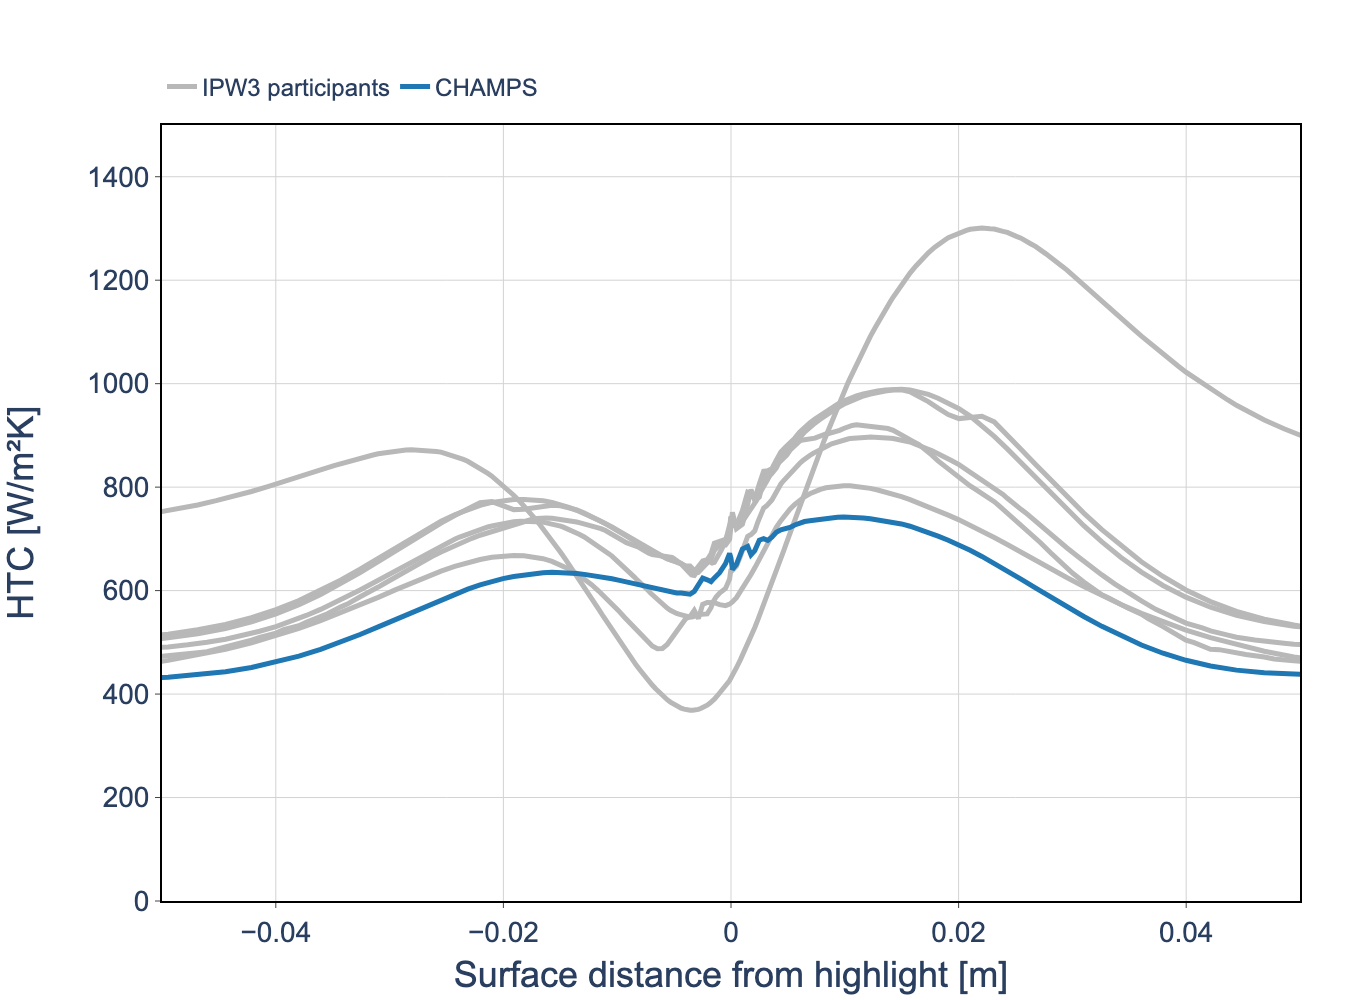
\includegraphics[
        width=\textwidth,
        trim={0cm 0cm 1cm 3.2cm},
        clip
    ]
    {FIGURES/ONERAM6/HTC/tc_oneram6_L1_htc_vs_s_slice_0p75_roughness_1mm.png}
\end{column}

% ------------------------------------------------------------
% y = 1.40 m
% ------------------------------------------------------------
\begin{column}{0.33\textwidth}
    \centering
    \textbf{$y=1.40$ m}

    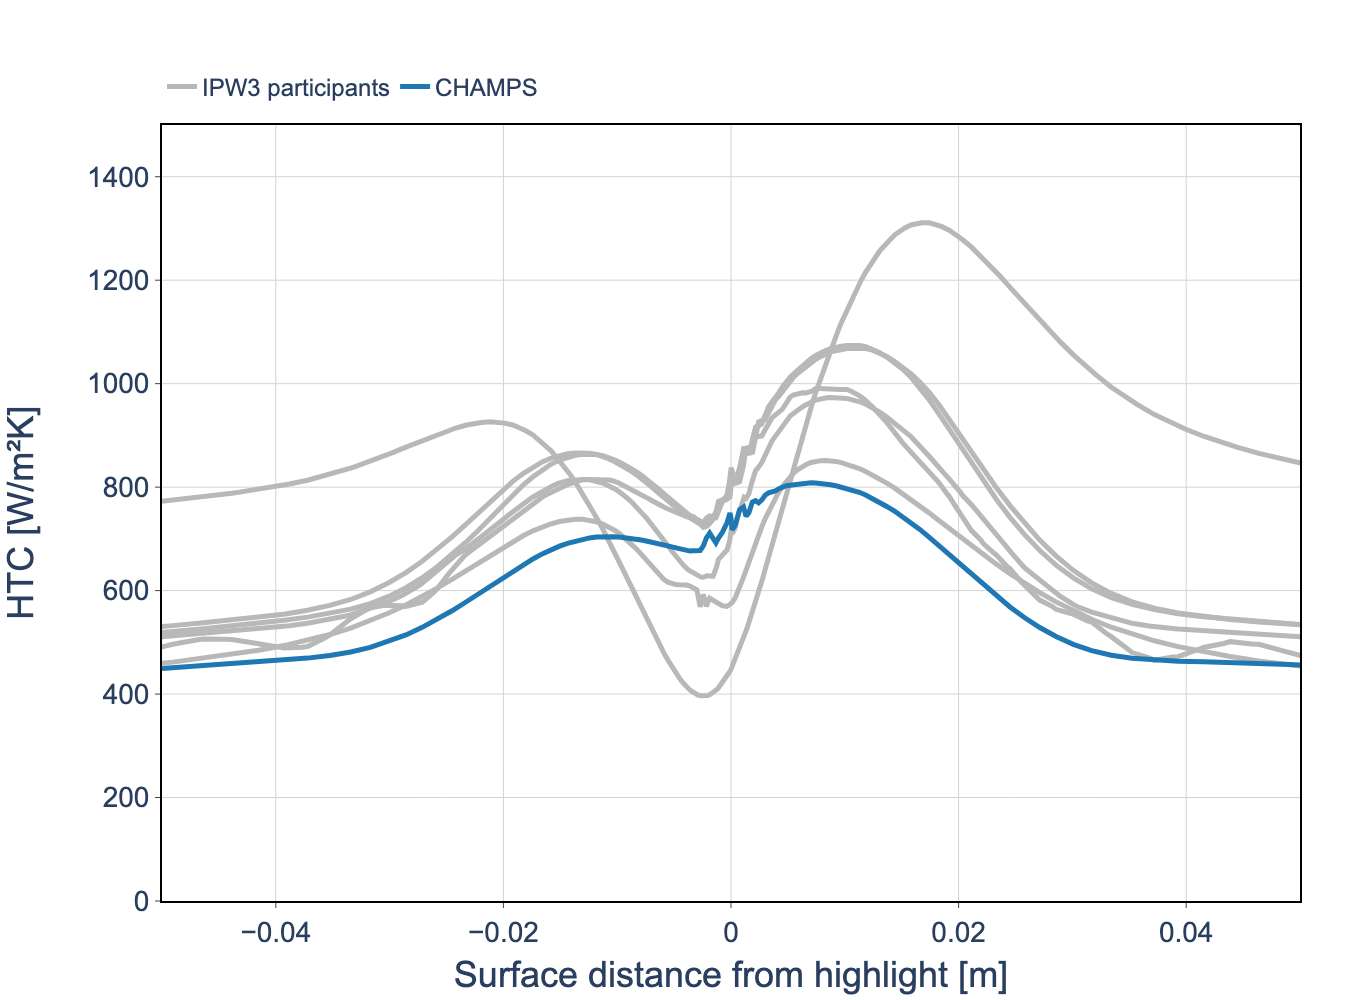
\includegraphics[
        width=\textwidth,
        trim={0cm 0cm 1cm 3.2cm},
        clip
    ]
    {FIGURES/ONERAM6/HTC/tc_oneram6_L1_htc_vs_s_slice_1p4_roughness_1mm.png}
\end{column}

\end{columns}

\end{frame}

% ============================================================
% BACKUP -- ONERA M6 Thermodynamics
% ============================================================

\begin{frame}{\small ONERA M6 -- Surface Thermodynamics ($y=0.75$ m)}
\scriptsize

\vspace{-0.20cm}

\begin{columns}[T,onlytextwidth]

% ------------------------------------------------------------
% Surface Temperature
% ------------------------------------------------------------
\begin{column}{0.50\textwidth}
    \centering
    \textbf{Surface Temperature}

    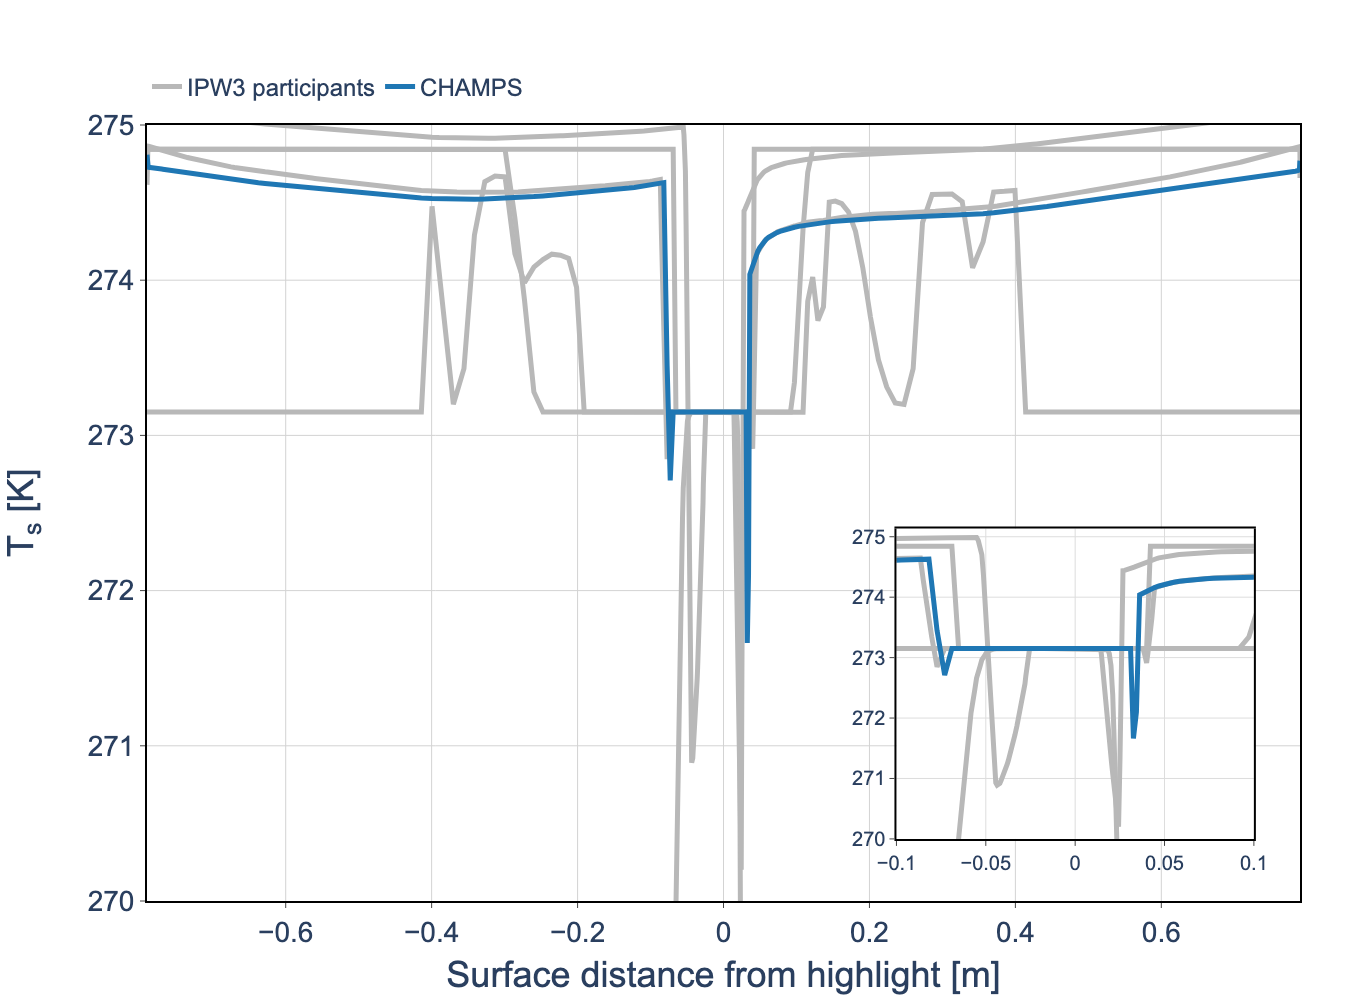
\includegraphics[
        width=\textwidth,
        trim={0cm 0cm 1cm 3.2cm},
        clip
    ]
    {FIGURES/ONERAM6/SURF_TEMP_FF/tc_oneram6_L1_surface_temperature_vs_s_slice_0p75_roughness_1mm.png}
\end{column}

% ------------------------------------------------------------
% Freezing Fraction
% ------------------------------------------------------------
\begin{column}{0.50\textwidth}
    \centering
    \textbf{Freezing Fraction}

    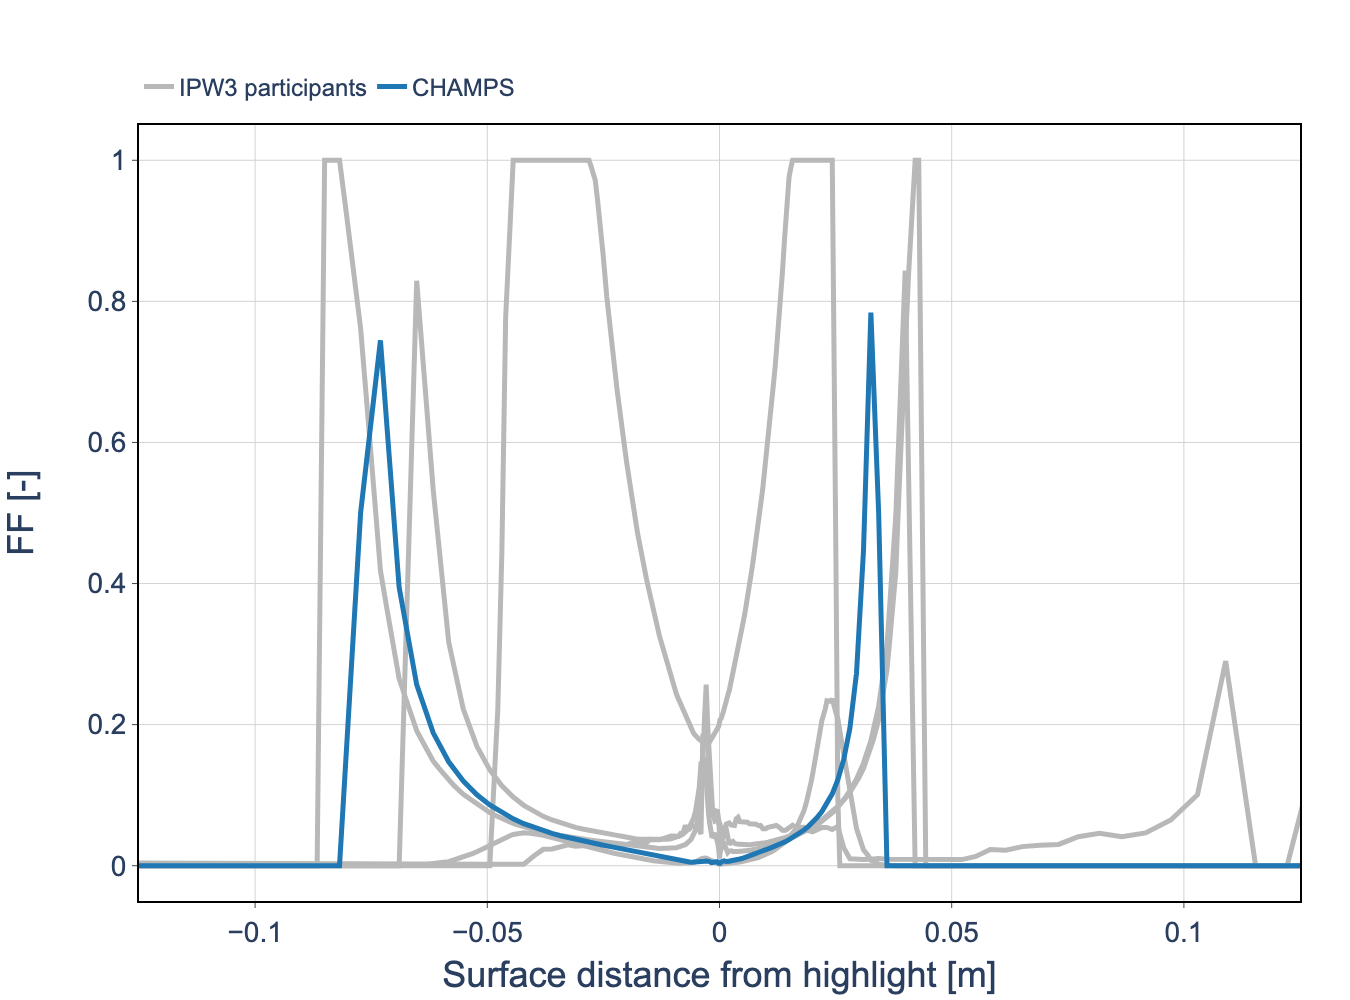
\includegraphics[
        width=\textwidth,
        trim={0cm 0cm 1cm 3.2cm},
        clip
    ]
    {FIGURES/ONERAM6/SURF_TEMP_FF/tc_oneram6_L1_freezing_fraction_vs_s_slice_0p75_roughness_1mm.png}
\end{column}

\end{columns}

\end{frame}

% ============================================================
% BACKUP -- ONERA M6 -- Surface-Normal Update
% ============================================================

\begin{frame}{\small ONERA M6 -- Effect of Surface-Normal Update}
\scriptsize

\vspace{-0.20cm}

\begin{columns}[T,onlytextwidth]

% ------------------------------------------------------------
% y = 0.10 m
% ------------------------------------------------------------
\begin{column}{0.33\textwidth}
    \centering
    \textbf{$y=0.10$ m}

    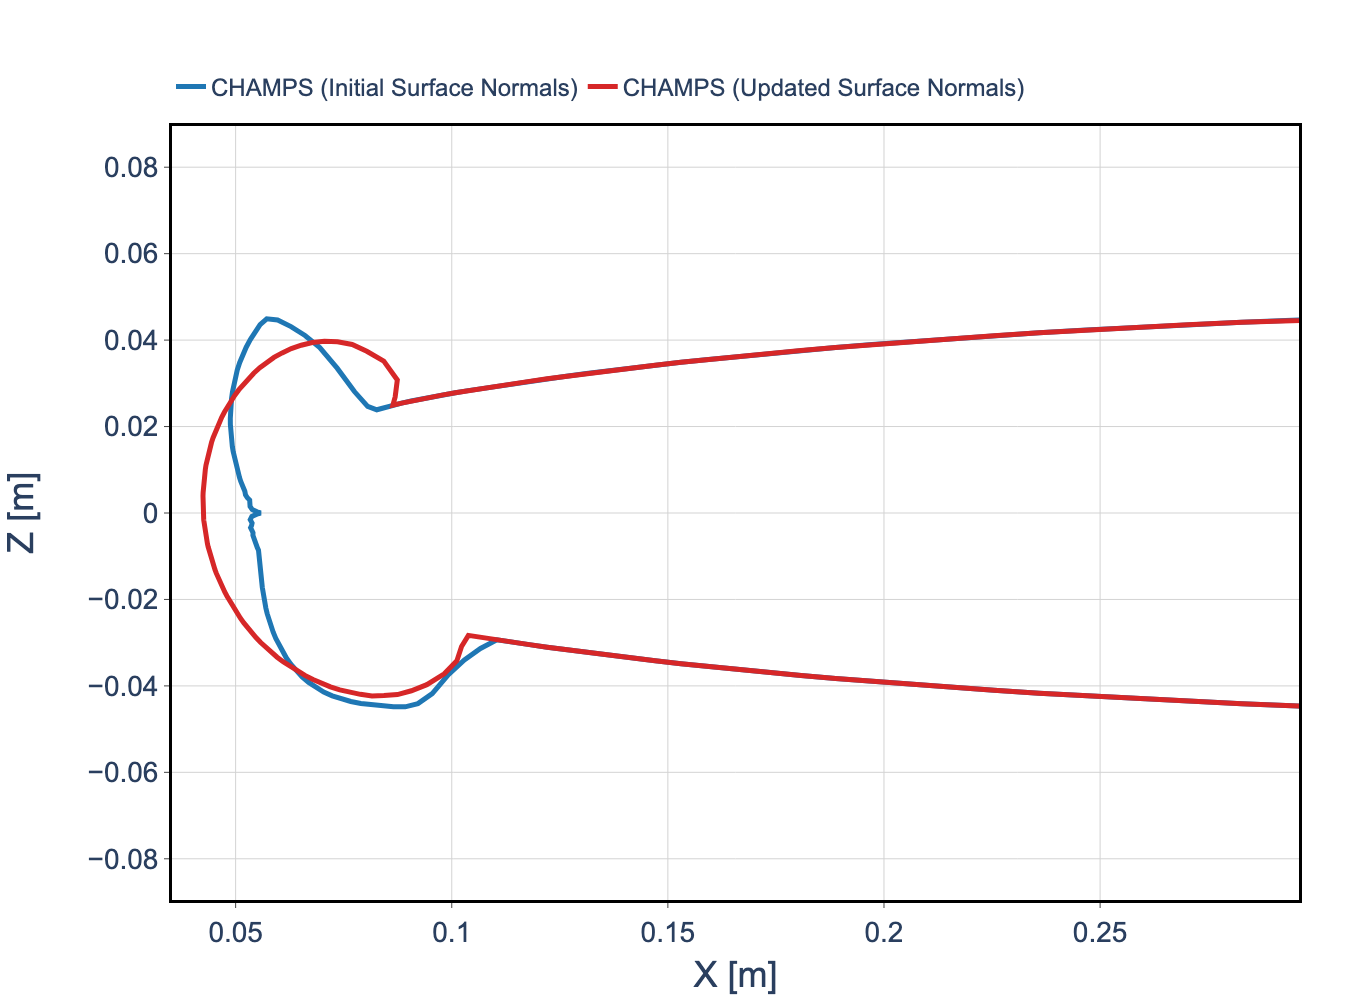
\includegraphics[
        width=\textwidth,
        trim={0cm 0cm 0cm 2.5cm},
        clip
    ]
    {FIGURES/ONERAM6/ICE_SHAPES/tc_oneram6_L1_single_layer_ice_shape_slice_0p1_bins15_normals_comparison.png}
\end{column}

% ------------------------------------------------------------
% y = 0.75 m
% ------------------------------------------------------------
\begin{column}{0.33\textwidth}
    \centering
    \textbf{$y=0.75$ m}

    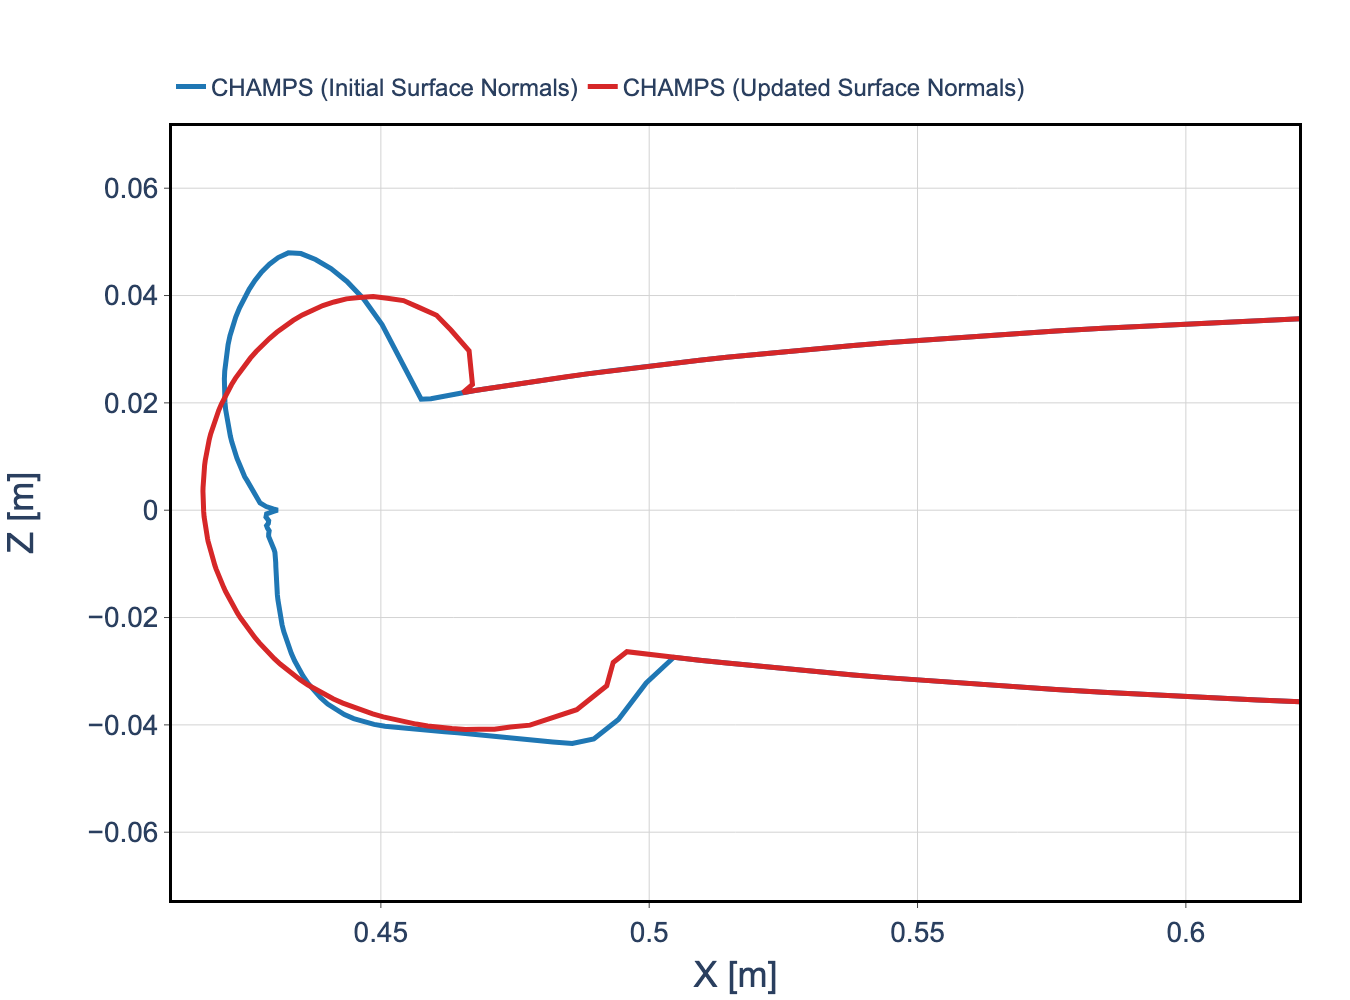
\includegraphics[
        width=\textwidth,
        trim={0cm 0cm 0cm 2.5cm},
        clip
    ]
    {FIGURES/ONERAM6/ICE_SHAPES/tc_oneram6_L1_single_layer_ice_shape_slice_0p75_bins15_normals_comparison.png}
\end{column}

% ------------------------------------------------------------
% y = 1.40 m
% ------------------------------------------------------------
\begin{column}{0.33\textwidth}
    \centering
    \textbf{$y=1.40$ m}

    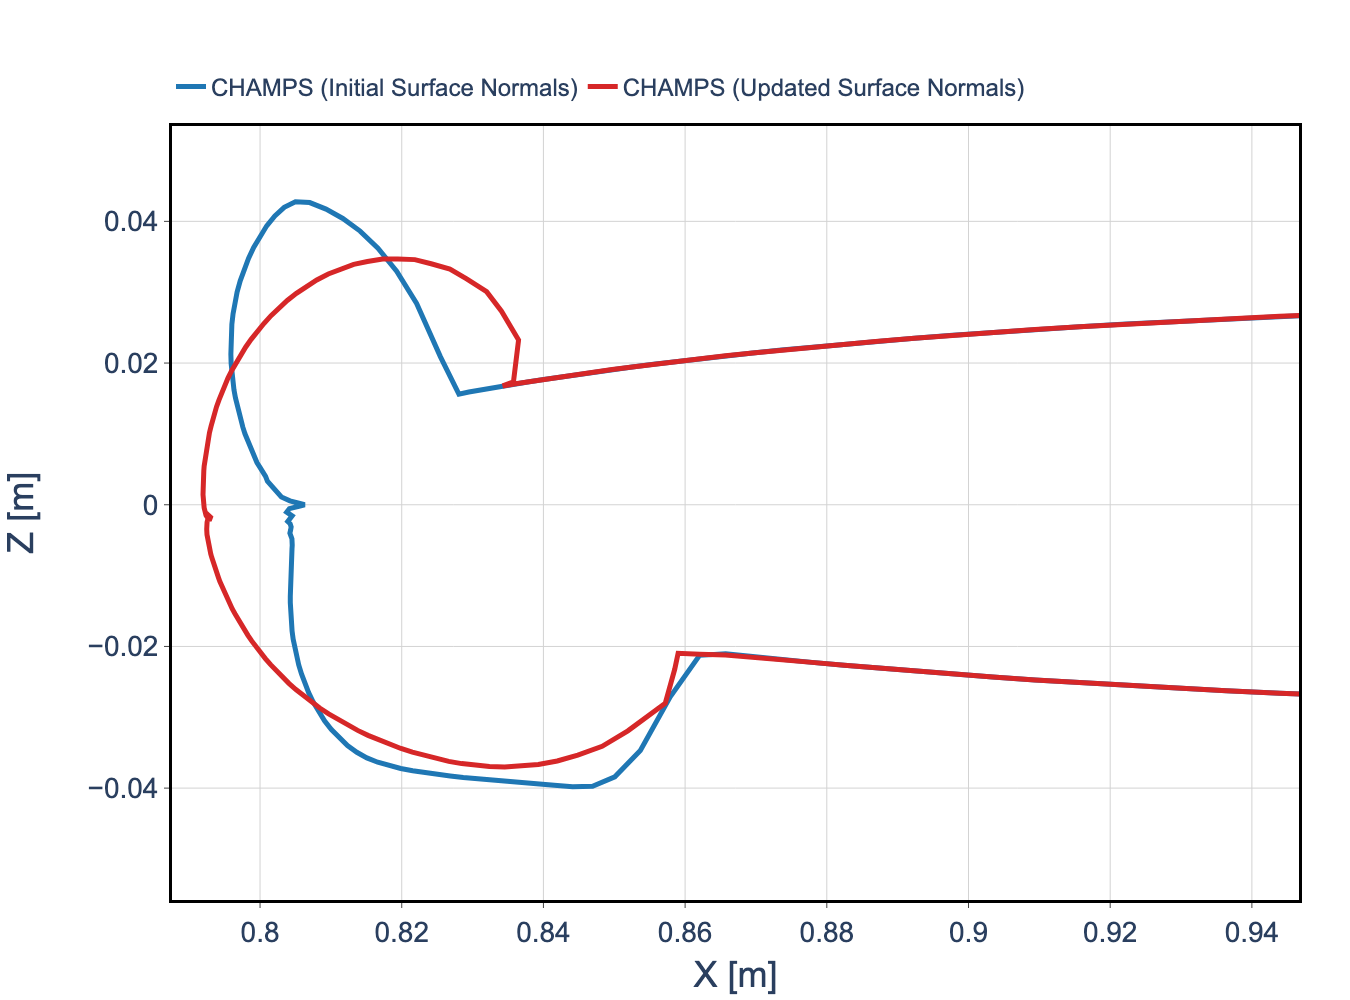
\includegraphics[
        width=\textwidth,
        trim={0cm 0cm 0cm 2.5cm},
        clip
    ]
    {FIGURES/ONERAM6/ICE_SHAPES/tc_oneram6_L1_single_layer_ice_shape_slice_1p4_bins15_normals_comparison.png}
\end{column}

\end{columns}

\end{frame}


% ============================================================
% CHAMPS -- LEVEL-SET GEOMETRY EVOLUTION
% ============================================================

\begin{frame}[c]{\small CHAMPS -- Multilayer Level-Set Evolution}
\scriptsize

\centering

% ============================================================
% STEP 1 -- GENERATE LEVEL-SET MESH
% ============================================================
\only<1>{

% Framework -- Step 1 highlighted
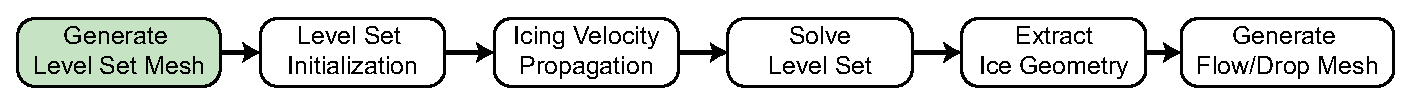
\includegraphics[
    width=0.95\textwidth
]{FIGURES/LS_FRAMEWORK/LS_STEP_1.eps}

\vspace{0.20cm}

\begin{block}{\scriptsize Generate Level-Set Mesh}
A dedicated level-set mesh is generated to avoid the restrictive
time-step requirements of the highly refined near-wall RANS mesh.
The mesh is adapted to encompass the expected ice-thickness extent.
\end{block}

\vspace{0.15cm}

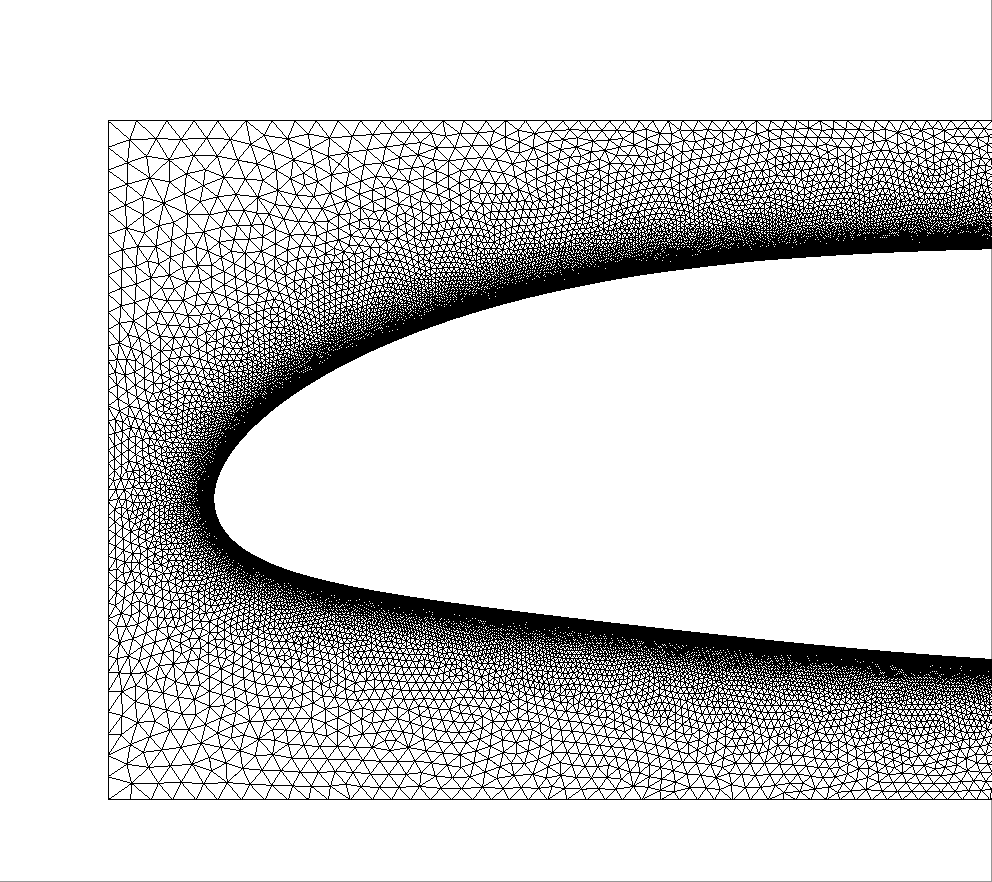
\includegraphics[
    width=0.4\textwidth,
    trim={0cm 0.1cm 3cm 3cm},
    clip
]{FIGURES/LS_FRAMEWORK/MESH_ADAPTATION.png}

}

% ============================================================
% STEP 2 -- LEVEL-SET INITIALIZATION
% ============================================================
\only<2>{

% Framework -- Step 2 highlighted
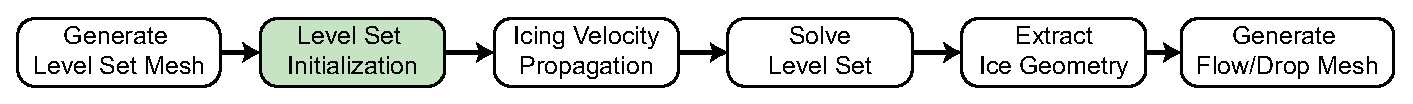
\includegraphics[
    width=0.95\textwidth
]{FIGURES/LS_FRAMEWORK/LS_STEP_2.eps}

\vspace{0.20cm}

\begin{block}{\scriptsize Level-Set Initialization}
The level-set field is initialized as a signed-distance function
from the current ice--air interface using an \textbf{Eikonal-based
wall-distance method} or an equivalent wall-distance technique.
\end{block}

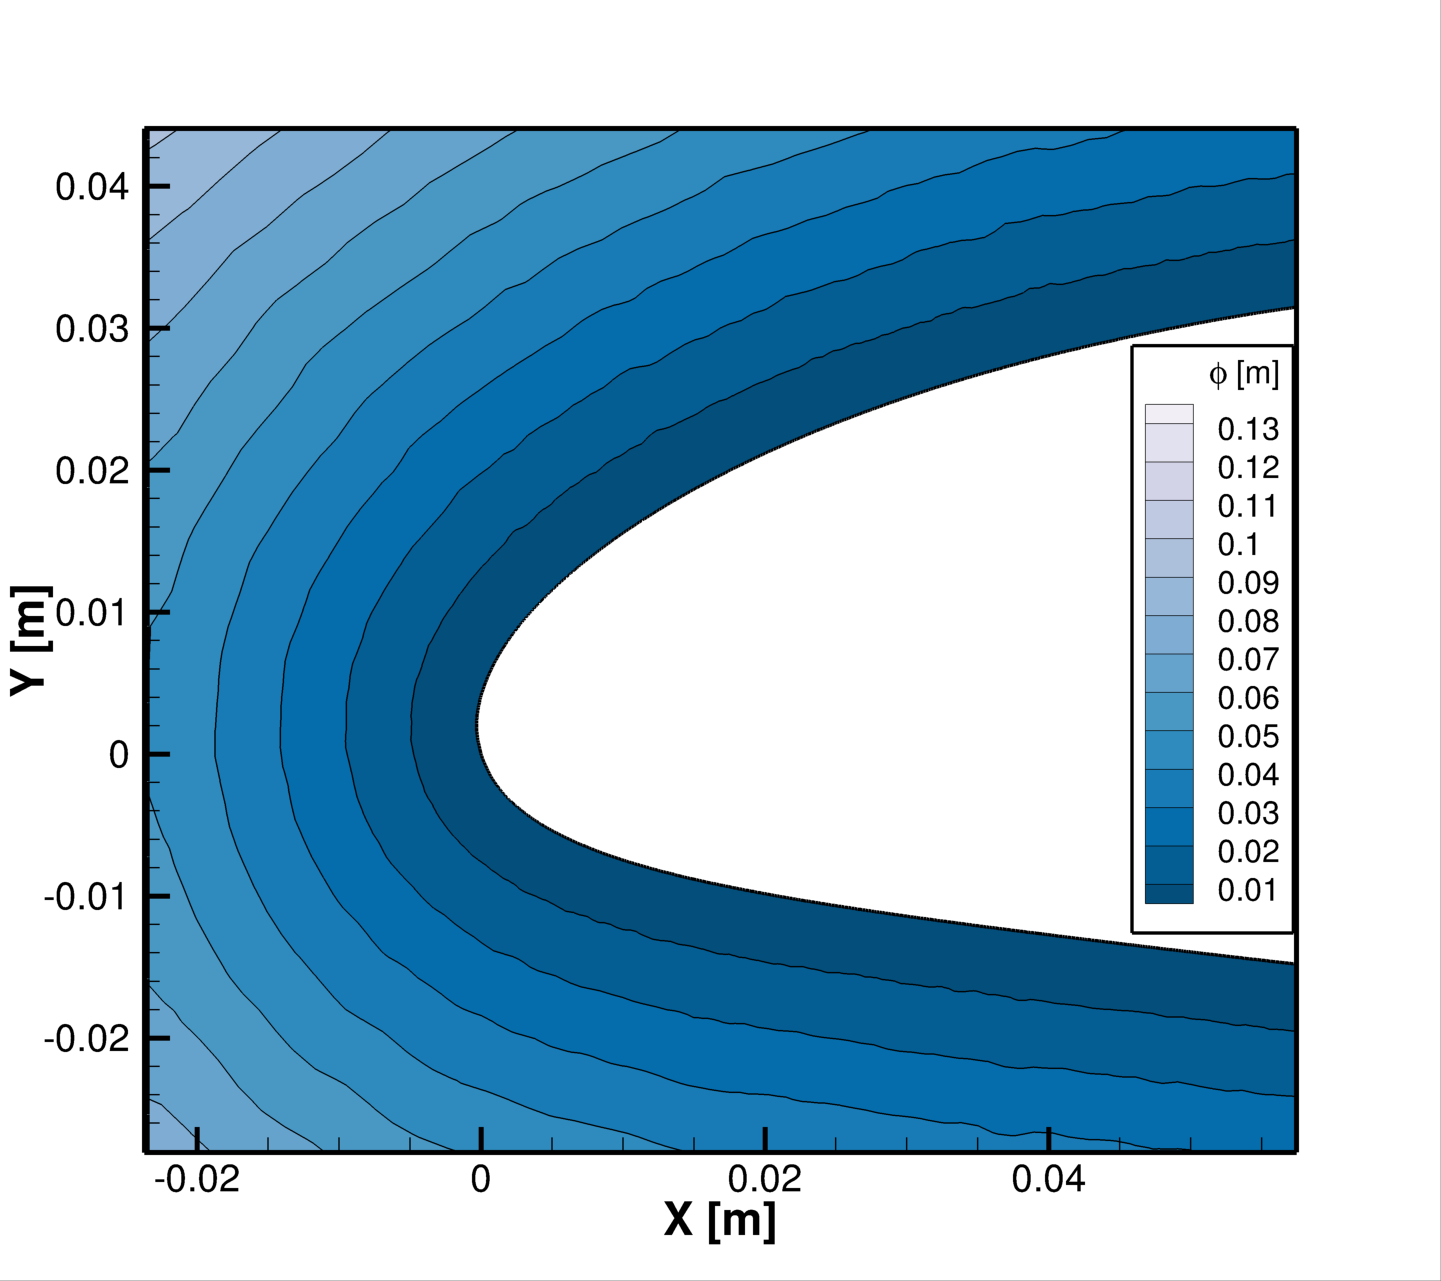
\includegraphics[
    width=0.35\textwidth,
    trim={0cm 0.1cm 3cm 3cm},
    clip
]{FIGURES/LS_FRAMEWORK/EIKONAL.png}

}

% ============================================================
% STEP 3 -- ICING VELOCITY PROPAGATION
% ============================================================
\only<3>{

% Framework -- Step 3 highlighted
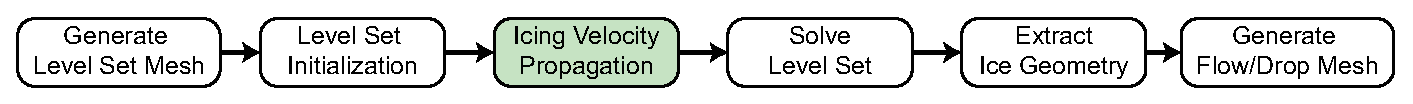
\includegraphics[
    width=0.95\textwidth
]{FIGURES/LS_FRAMEWORK/LS_STEP_3.eps}

\vspace{0.20cm}

\begin{block}{\scriptsize Icing Velocity Propagation}
The interface velocity magnitude,
$V_{\mathrm{ice}} = h_{\mathrm{ice}}/\Delta t_{\mathrm{layer}}$,
is propagated from the ice--air interface into the level-set domain.
The interface velocity is then constructed using the level-set normal:
\[
\boldsymbol{V}
=
V_{\mathrm{ice}}\,\boldsymbol{n}_{\phi}.
\]
\end{block}


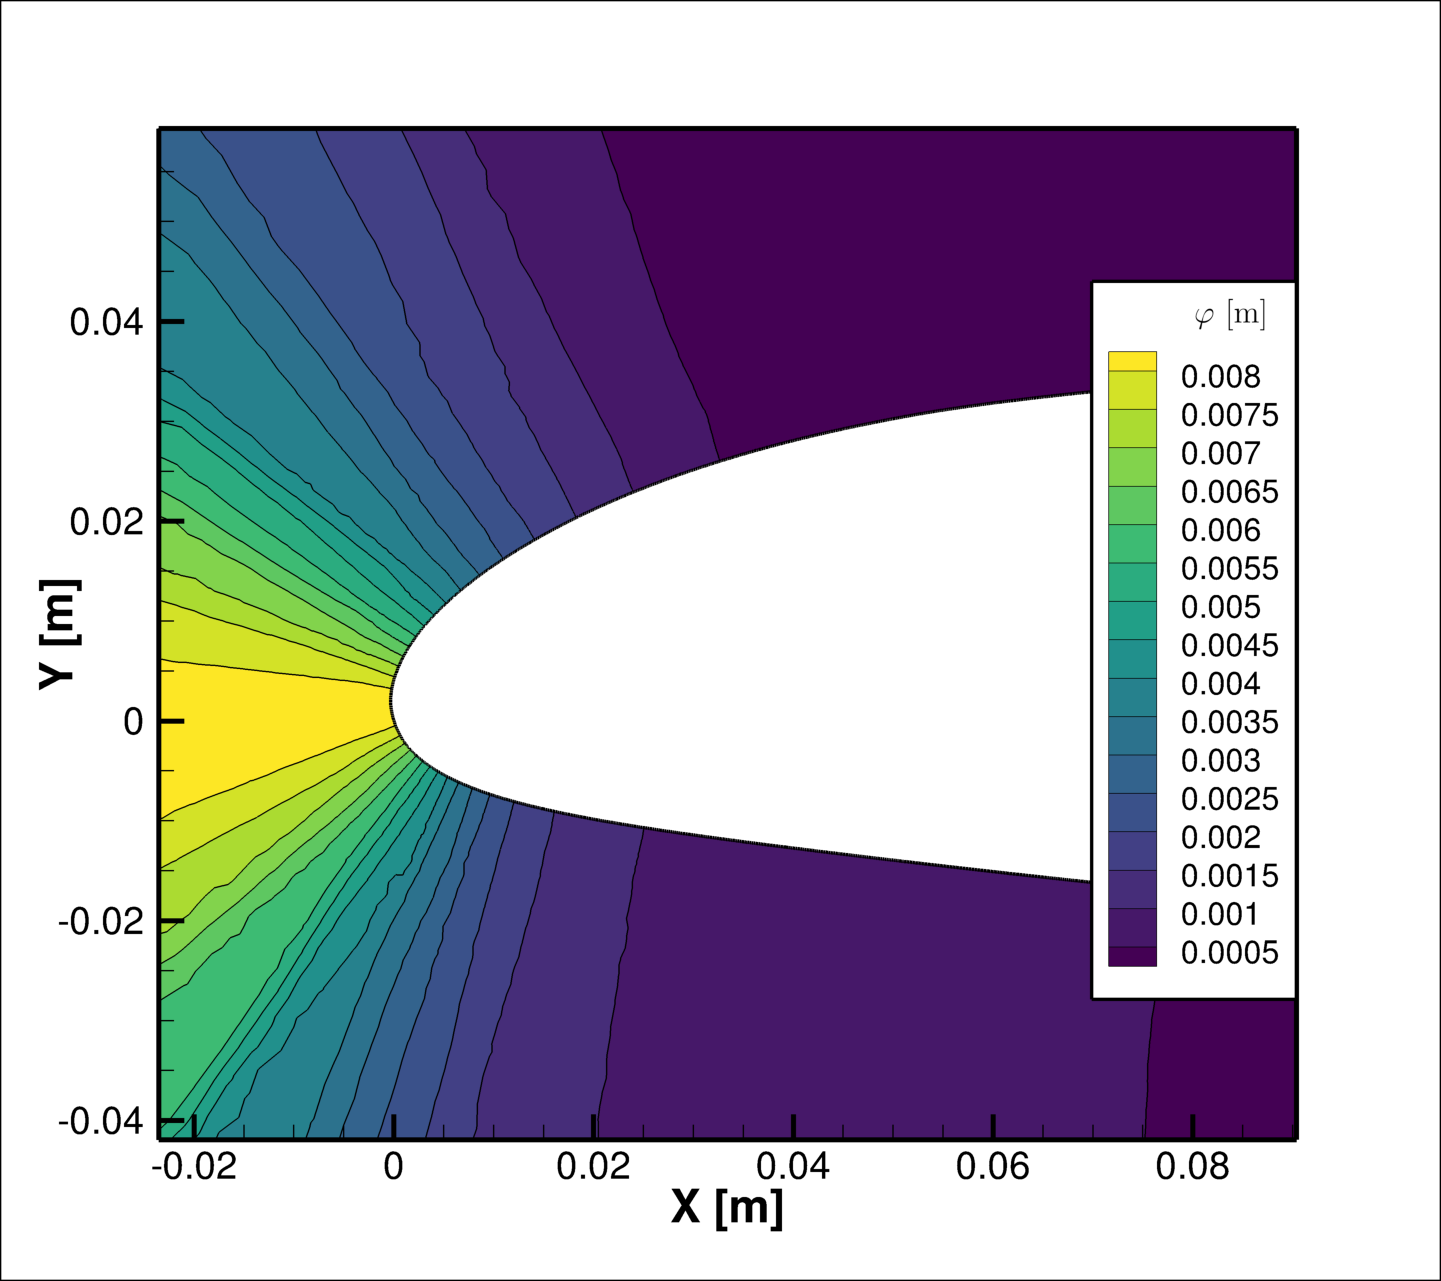
\includegraphics[
    width=0.35\textwidth,
    trim={0.1cm 0.1cm 3cm 3cm},
    clip
]{FIGURES/LS_FRAMEWORK/PROPAGATION.png}

}

% ============================================================
% STEP 4 -- SOLVE LEVEL SET
% ============================================================
\only<4>{

% Framework -- Solve Level Set highlighted
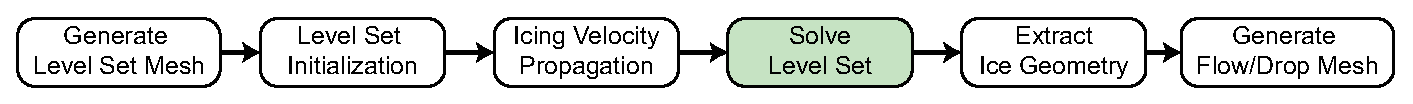
\includegraphics[
    width=0.95\textwidth
]{FIGURES/LS_FRAMEWORK/LS_STEP_4.eps}

\vspace{0.20cm}

\begin{block}{\scriptsize Solve Level Set -- Rosenbrock--Wanner (ROW) Scheme}

\begin{itemize}

    \item The level-set transport equation is advanced using a
    \textbf{two-stage Rosenbrock--Wanner (ROW) semi-implicit scheme}:

    \vspace{-0.10cm}

    \[
    \phi^{n+1}
    =
    \phi^n+\sum_{j=1}^{s}m_jS_j,
    \qquad
    \left(
    \frac{\boldsymbol{I}}{\gamma\Delta t}
    +\boldsymbol{J}
    \right)^n S_i
    =
    -R\left(
    \phi^n+\sum_{j=1}^{i-1}a_{ij}S_j
    \right).
    \]

    \vspace{-0.10cm}

    \item The ROW scheme has demonstrated
    \textbf{excellent performance for flow time integration in CHAMPS},
    providing improved stability and allowing larger time steps;
    it was therefore adopted for the level-set equation.

    \item At each ROW stage, a \textbf{linear system} is solved iteratively
    using \textbf{GMRES}:
    \[
    \underbrace{
    \left(
    \frac{\boldsymbol{I}}{\gamma\Delta t}
    +\boldsymbol{J}
    \right)^n}_{\boldsymbol{A}}
    S_i
    =
    \underbrace{
    -R\left(
    \phi^n+\sum_{j=1}^{i-1}a_{ij}S_j
    \right)}_{\boldsymbol{b}_i}.
    \]

\end{itemize}

\vspace{-0.10cm}

{\tiny
\textbf{*}
$\phi^n$: level-set solution;
$S_i$: stage increment;
$s$: number of ROW stages;
$m_j$, $a_{ij}$: ROW coefficients;
$\gamma$: ROW parameter;
$\Delta t$: time step;
$\boldsymbol{I}$: identity matrix;
$R(\phi)$: spatial residual;
$\boldsymbol{J}=\partial R/\partial\phi$: residual Jacobian.
}

\end{block}

}

% ============================================================
% STEP 5 -- EXTRACT ICE GEOMETRY
% ============================================================
\only<5>{

% Framework -- Step 5 highlighted
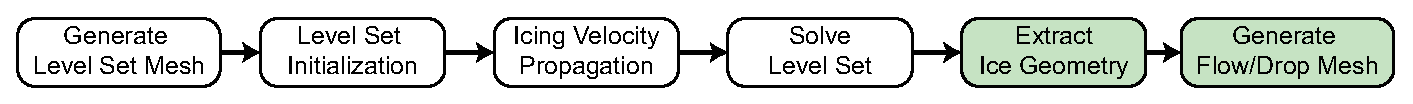
\includegraphics[
    width=0.95\textwidth
]{FIGURES/LS_FRAMEWORK/LS_STEP_5.eps}

\vspace{0.20cm}

\begin{block}{\scriptsize Extract Ice Geometry \& Generate Volume Mesh}
The updated ice surface is extracted from the volumetric level-set
solution as the $\phi=0$ isosurface using \textbf{MMG}. A new
\textbf{volume mesh} is then generated around the updated ice geometry
using \textbf{Pointwise Python scripts}.
\end{block}

\vspace{0.15cm}

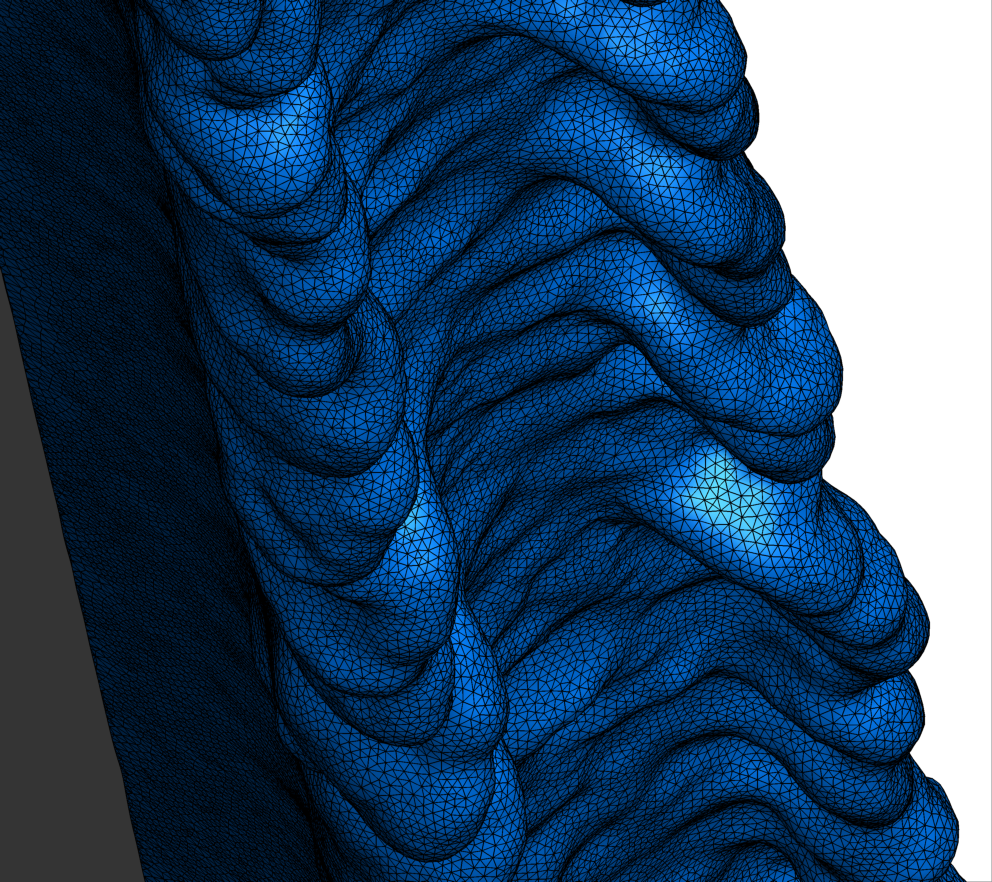
\includegraphics[
    width=0.4\textwidth
]{FIGURES/LS_FRAMEWORK/CLIPPED_ICE_SHAPE_CASE_362_3.png}

}

\end{frame}


\begin{frame}[allowframebreaks]{\small References}
\scriptsize
\nocite{*}
\bibliography{references}
\end{frame}

\end{document}
